%%%%%%%%%%%%%%%%%%%%%%%%%%%%%%%%%%%%%%%%%
% Masters/Doctoral Thesis 
% LaTeX Template
% Version 2.5 (27/8/17)
%
% This template was downloaded from:
% http://www.LaTeXTemplates.com
%
% Version 2.x major modifications by:
% Vel (vel@latextemplates.com)
%
% This template is based on a template by:
% Steve Gunn (http://users.ecs.soton.ac.uk/srg/softwaretools/document/templates/)
% Sunil Patel (http://www.sunilpatel.co.uk/thesis-template/)
%
% Template license:
% CC BY-NC-SA 3.0 (http://creativecommons.org/licenses/by-nc-sa/3.0/)
%
%%%%%%%%%%%%%%%%%%%%%%%%%%%%%%%%%%%%%%%%%

%----------------------------------------------------------------------------------------
%	PACKAGES AND OTHER DOCUMENT CONFIGURATIONS
%----------------------------------------------------------------------------------------

\documentclass[
11pt, % The default document font size, options: 10pt, 11pt, 12pt
oneside, % Two side (alternating margins) for binding by default, uncomment to switch to one side
english, % ngerman for German
onehalfspacing, % Single line spacing, alternatives: onehalfspacing or doublespacing
%draft, % Uncomment to enable draft mode (no pictures, no links, overfull hboxes indicated)
%nolistspacing, % If the document is onehalfspacing or doublespacing, uncomment this to set spacing in lists to single
%liststotoc, % Uncomment to add the list of figures/tables/etc to the table of contents
%toctotoc, % Uncomment to add the main table of contents to the table of contents
%parskip, % Uncomment to add space between paragraphs
%nohyperref, % Uncomment to not load the hyperref package
headsepline, % Uncomment to get a line under the header
chapterinoneline, % Uncomment to place the chapter title next to the number on one line
%consistentlayout, % Uncomment to change the layout of the declaration, abstract and acknowledgements pages to match the default layout
]{MastersDoctoralThesis} % The class file specifying the document structure

\setcounter{tocdepth}{2} % set contents list depth to 2

\usepackage[utf8]{inputenc} % Required for inputting international characters
\usepackage[T1]{fontenc} % Output font encoding for international characters

\usepackage{mathpazo} % Use the Palatino font by default
\usepackage[scr=boondoxo, scrscaled=.98]{mathalfa}



\DeclareFontFamily{U}{BOONDOX-calo}{\skewchar\font=45 }
\DeclareFontShape{U}{BOONDOX-calo}{m}{n}{
  <-> s*[1.05] BOONDOX-r-calo}{}
\DeclareFontShape{U}{BOONDOX-calo}{b}{n}{
  <-> s*[1.05] BOONDOX-b-calo}{}
\DeclareMathAlphabet{\mathcalboondox}{U}{BOONDOX-calo}{m}{n}
\SetMathAlphabet{\mathcalboondox}{bold}{U}{BOONDOX-calo}{b}{n}
\DeclareMathAlphabet{\mathbcalboondox}{U}{BOONDOX-calo}{b}{n}


\usepackage[lined, boxed]{algorithm2e} %Algorithm environment package
\usepackage{amsmath}
\usepackage{amsfonts}
\usepackage{amssymb} 
\usepackage{array}
\usepackage{booktabs}
\usepackage{caption}
\usepackage{color}
\usepackage{collcell}
\usepackage{graphicx}
\usepackage{hyperref}
\usepackage{longtable} 
\usepackage{physics}
\usepackage{makecell} % Multirow in table header
\usepackage{mathtools}
\usepackage{miller}   % Miller indices package
\usepackage{multirow} % Multirow in tables package
\usepackage[super]{nth}
\usepackage{setspace}
\usepackage{etoolbox}
\usepackage{xargs}                      % Use more than one optional parameter in a new commands
\usepackage{rotating}   % landscape figures


\usepackage{combelow}


% All the notes
\usepackage[colorinlistoftodos,prependcaption,textsize=tiny]{todonotes}
\newcommandx{\unsure}[2][1=]{\todo[linecolor=red,backgroundcolor=red!25,bordercolor=red,#1]{#2}}
\newcommandx{\change}[2][1=]{\todo[linecolor=blue,backgroundcolor=blue!25,bordercolor=blue,#1]{#2}}
\newcommandx{\info}[2][1=]{\todo[linecolor=OliveGreen,backgroundcolor=OliveGreen!25,bordercolor=OliveGreen,#1]{#2}}
\newcommandx{\improvement}[2][1=]{\todo[linecolor=Plum,backgroundcolor=Plum!25,bordercolor=Plum,#1]{#2}}
\newcommandx{\thiswillnotshow}[2][1=]{\todo[disable,#1]{#2}}


% align complex numbers in tables with N
\sisetup{
output-complex-root = \ensuremath{\mathrm{i}},
complex-root-position = before-number
}

\newlength{\WidestRealNum}
\settowidth{\WidestRealNum}{$99999$}
\newcommand*{\ApplyNumFormatting}[1]{%
\IfSubStr{#1}{+}{%
     \StrBefore{#1}{+}[\RealPart]}{%
     \IfSubStr[2]{#1}{-}{%
          \StrBefore[2]{#1}{-}[\RealPart]}{%
          \StrBefore{#1}{-}[\RealPart]}%
     }
     \StrBehind{#1}{i}[\ImagPart]%

\IfSubStr{#1}{+}{%
    $\makebox[\WidestRealNum][r]{$\RealPart$} + i\,\ImagPart$}{%
    $\makebox[\WidestRealNum][r]{$\RealPart$} - i\,\ImagPart$}
}%

\newcolumntype{N}{>{\collectcell\ApplyNumFormatting}l<{\endcollectcell}}




% Crystallographic symmetry font symbols
\DeclareFontFamily{U}{cry}{\hyphenchar\font=-1}
\DeclareFontShape{U}{cry}{m}{n}{ <-> cryst}{}
\newcommand{\cry}[1]{{\usefont{U}{cry}{m}{n} \symbol{#1}}}

% Ignore line spacing in equations
\AtBeginEnvironment{equation}{\leavevmode\singlespace}
\AfterEndEnvironment{equation}{\endsinglespace\vskip0.5\baselineskip\noindent\ignorespaces}
\AtBeginEnvironment{equation*}{\leavevmode\singlespace}
\AfterEndEnvironment{equation*}{\endsinglespace\vskip0.5\baselineskip\noindent\ignorespaces}
\AtBeginEnvironment{align}{\leavevmode\singlespace}
\AfterEndEnvironment{align}{\endsinglespace\vskip0.5\baselineskip\noindent\ignorespaces}
\AtBeginEnvironment{algorithm}{\leavevmode\singlespace}
\AfterEndEnvironment{algorithm}{\endsinglespace\vskip0.5\baselineskip\noindent\ignorespaces}



% Fix algorithm caption
\renewcommand{\AlCapSty}{\textsc}
\SetAlgoCaptionLayout{centerlast} 
\SetAlCapNameFnt{\small}
\SetAlCapFnt{\small}
\SetAlCapSkip{0.8ex}

% Define table heads 
\newcommand{\keyword}[1]{\textbf{#1}}
\newcommand{\tabhead}[1]{\textbf{#1}}
\newcommand{\code}[1]{\texttt{#1}}
\newcommand{\file}[1]{\texttt{\bfseries#1}}
\newcommand{\option}[1]{\texttt{\itshape#1}}

%---------Elena's new commands--------------------
\newcommand{\etal}{\textit{et al}. }
\newcommand{\ie}{\textit{i}.\textit{e}., }
\newcommand{\eg}{\textit{e}.\textit{g}. }
%------------------------------------------------

\usepackage[backend=bibtex,style=alphabetic,natbib=true]{biblatex} % Use the bibtex backend with the authoryear citation style (which resembles APA)
\addbibresource{Biblio/intro}
\addbibresource{Biblio/theory}
\addbibresource{Biblio/diffraction}
\addbibresource{Biblio/ecci}
\addbibresource{Biblio/tkd}
\usepackage[autostyle=true]{csquotes} % Required to generate language-dependent quotes in the bibliography

%----------------------------------------------------------------------------------------
%	MARGIN SETTINGS
%----------------------------------------------------------------------------------------

\geometry{
	paper=a4paper, % Change to letterpaper for US letter
	inner=3.5cm, % Inner margin
	outer=2.5cm, % Outer margin
	bindingoffset=.5cm, % Binding offset
	top=2.0cm, % Top margin
	bottom=4.0cm, % Bottom margin
	%showframe, % Uncomment to show how the type block is set on the page
}

%----------------------------------------------------------------------------------------
%	THESIS INFORMATION
%----------------------------------------------------------------------------------------

\thesistitle{Dynamical models for novel diffraction techniques in SEM} % Your thesis title, this is used in the title and abstract, print it elsewhere with \ttitle
\supervisor{Dr. Ben \textsc{Hourahine}\\
            Dr. Carol \textsc{Trager-Cowan}} % Your supervisor's name, this is used in the title page, print it elsewhere with \supname
\examiner{} % Your examiner's name, this is not currently used anywhere in the template, print it elsewhere with \examname
\degree{Doctor of Philosophy} % Your degree name, this is used in the title page and abstract, print it elsewhere with \degreename
\author{Elena \textsc{Pascal}} % Your name, this is used in the title page and abstract, print it elsewhere with \authorname
\addresses{} % Your address, this is not currently used anywhere in the template, print it elsewhere with \addressname

\subject{Physics} % Your subject area, this is not currently used anywhere in the template, print it elsewhere with \subjectname
\keywords{} % Keywords for your thesis, this is not currently used anywhere in the template, print it elsewhere with \keywordnames
\university{\href{https://www.strath.ac.uk/}{University of Strathclyde}} % Your university's name and URL, this is used in the title page and abstract, print it elsewhere with \univname
\department{\href{https://www.strath.ac.uk/research/subjects/physics/}{Department of Physics}} % Your department's name and URL, this is used in the title page and abstract, print it elsewhere with \deptname
\group{\href{http://ssd.phys.strath.ac.uk/}{Semiconductor Spectroscopy and Devices Group}} % Your research group's name and URL, this is used in the title page, print it elsewhere with \groupname
\faculty{\href{https://www.strath.ac.uk/science/}{Science}} % Your faculty's name and URL, this is used in the title page and abstract, print it elsewhere with \facname

\AtBeginDocument{
\hypersetup{pdftitle=\ttitle} % Set the PDF's title to your title
\hypersetup{pdfauthor=\authorname} % Set the PDF's author to your name
\hypersetup{pdfkeywords=\keywordnames} % Set the PDF's keywords to your keywords
}

\begin{document}

\frontmatter % Use roman page numbering style (i, ii, iii, iv...) for the pre-content pages

\pagestyle{plain} % Default to the plain heading style until the thesis style is called for the body content

%----------------------------------------------------------------------------------------
%	TITLE PAGE
%----------------------------------------------------------------------------------------

\begin{titlepage}
\begin{center}
\vspace*{-.18\textheight}
\begin{flushright}
 \includegraphics{logo.pdf}
 \end{flushright} % University/department logo - uncomment to place it

\vspace*{.06\textheight}
{\scshape\LARGE \univname\par}\vspace{1.5cm} % University name
\textsc{\Large Doctoral Thesis}\\[0.5cm] % Thesis type

\HRule \\[0.4cm] % Horizontal line
{\huge \bfseries \ttitle\par}\vspace{0.4cm} % Thesis title
\HRule \\[1.5cm] % Horizontal line
 
\begin{minipage}[t]{0.4\textwidth}
\begin{flushleft} \large
\emph{Author:}\\
\href{https://pure.strath.ac.uk/portal/en/persons/elena-pascal(f3ebee32-ba1a-417f-9d8e-5bdc5a801ce4).html}
{\authorname} % Author name - remove the \href bracket to remove the link
\end{flushleft}
\end{minipage}
\begin{minipage}[t]{0.4\textwidth}
\begin{flushright} \large
\emph{Supervisor:} \\
\href{https://www.strath.ac.uk/staff/hourahinebenjamindr/}
{\supname} % Supervisor name - remove the \href bracket to remove the link  
\end{flushright}
\end{minipage}\\[3cm]
 
\large \textit{A thesis submitted in fulfilment of the requirements\\ for the degree of \degreename}\\[0.3cm] % University requirement text
\textit{in the}\\[0.4cm]
\groupname\\\deptname\\%[2cm] % Research group name and department name
{\large \the\year}\\%[4cm] % Date

\end{center}
\end{titlepage}

%----------------------------------------------------------------------------------------
%	DECLARATION PAGE
%----------------------------------------------------------------------------------------

\begin{declaration}
%\addchaptertocentry{\authorshipname} % Add the declaration to the table of contents


\noindent I, \authorname, declare that this thesis titled, \enquote{\ttitle} and the work presented in it are my own. I confirm that:

\begin{itemize} 
\item This thesis is the result of the author’s original research. It has been composed by
the author and has not been previously submitted for examination which has led to
the award of a degree.

\item Where I have consulted the published work of others, this is always clearly attributed.
\item I have acknowledged all main sources of help.
\item Where the thesis is based on work done by myself jointly with others, I have made clear exactly what was done by others and what I have contributed myself.

\end{itemize}

The copyright of this thesis belongs to the author under the terms of the United
Kingdom Copyright Acts as qualified by University of Strathclyde Regulation 3.50.
Due acknowledgement must always be made of the use of any material contained
in, or derived from, this thesis.

\vfill

\noindent Signed:\\
\rule[0.5em]{25em}{0.5pt} % This prints a line for the signature
 
\noindent Date:\\
\rule[0.5em]{25em}{0.5pt} % This prints a line to write the date
\end{declaration}

\cleardoublepage

%----------------------------------------------------------------------------------------
%	QUOTATION PAGE
%----------------------------------------------------------------------------------------

\vspace*{0.2\textheight}

\noindent\enquote{\itshape The way the creative process works is that you first say something, and later, sometimes years later, you understand what you said.}\bigbreak

\hfill Daniel Kahneman

%----------------------------------------------------------------------------------------
%	ABSTRACT PAGE
%----------------------------------------------------------------------------------------

\begin{abstract}
%\addchaptertocentry{\abstractname} % Add the abstract to the table of contents

The scanning electron microscope is a powerful nanocharacterisation tool for a variety of materials including semiconductors and metals. Less known for its diffraction abilities than its transmission counterpart, scanning electron microscopy (SEM)  can be used in  a number of diffraction modalities to provide information on crystal imperfections at the nanoscale level. This comes with the added benefit of SEM requiring minimal sample preparation. %intro
Models for diffraction in the SEM are still being developed and improved, hence in this work I explore the physics and implementations of such models. %motivation
I focus on the two main branches of SEM diffraction techniques: incident beam channelling, or \textit{diffraction in}, powerful when it comes to resolving individual dislocations close to the surface; and back(/forward)scattering diffraction, or \textit{diffraction out}, which provides a variety of information about grain distribution, orientation and strain. Both of these diffraction modalities involve the same physical processes, so it makes sense to use the same models, namely dynamical scattering in the column approximation. %methods
I use the two beam Bloch waves approach for electron channelling contrast imaging (ECCI) of threading dislocations (TDs) normal to the surface in wurtzite group-III nitride materials. I also introduce and use the notion of ECC-strain to study crystal features and to predict the behaviour of  TDs contrast. 
For the electron back(/forward)scatter modality, I show the first application of the new energy-weighted dynamical scattering capabilities of EMsoft to study the novel transmission mode (TKD) of the SEM. %results
\end{abstract}

%----------------------------------------------------------------------------------------
%	ACKNOWLEDGEMENTS
%----------------------------------------------------------------------------------------

\begin{acknowledgements}
%\addchaptertocentry{\acknowledgementname} % Add the acknowledgements to the table of contents
%The acknowledgements and the people to thank go here, don't forget to include your project advisor\ldots

\vspace{2cm}
I want to thank the entire SSD group for being welcoming and generous with their time and for all the science and non-science conversations. I am thankful for all my wonderful office mates, Nouf for kindly teaching me basics when I started, Paul for unlimited wisdom, James for welcomed distractions. I also have to mention Stefano for taking me under his wing in the first two years, and trying to pass his polymath knowledge onto me; I only wish I made more of your time here. I do hold fond memories of our electron diffraction (sometimes heated) discussions.

I am incredibly indebted to my supervisors for guiding me at every step on this long and sometimes challenging journey. I have to thank Carol for taking me on the program and giving me a chance to do research. I am grateful to her for always being available to hear any concerns I might have. I think I struggled with a lot of impostor's syndrome, and while I still do, I know that having Ben as a supervisor helped a lot. I am truly indebted for Ben's patience of framing the work I did in a way that made it sound meaningful even when we both knew that PhD work is rarely impactful. I am also thankful for all the very last minute revisions and feedback. 

I am extremely grateful for the support of my partner, Gunnar, without whom I don't think this manuscript would exist. Thank you for believing I am strong all the times I did not. Thank you for not doubting for a second I will hand in a Thesis for all the times I did.  


Most importantly, I would like to thank my mother, who, despite having been denied further education, values it so greatly that it took surprisingly little convincing work to let me leave ten years ago, with only a precarious survival plan, for a foreign land in the pursuit of it.   


\end{acknowledgements}


%----------------------------------------------------------------------------------------
%	LIST OF CONTRIBUTIONS
%----------------------------------------------------------------------------------------
\begin{contributions}
%\addchaptertocentry{\contribname} % Add the contributions to the table of contents
%papers

\vspace{0.3cm}
\noindent{\Large Papers:}
\begin{itemize}
    \item \textbf{E Pascal}, S Singh, P  G Callahan, B Hourahine, C Trager-Cowan, M De Graef, \href{https://doi.org/10.1016/j.ultramic.2018.01.003}{\textit{Energy-weighted dynamical scattering simulations of electron diffraction modalities in the scanning electron microscope}}, Ultramicroscopy,  \textbf{187}, 2018, 98-106.

    
    \item \textbf{E Pascal}, B Hourahine, G Naresh-Kumar, K Mingard, C Trager-Cowan, \href{https://doi.org/10.1016/j.matpr.2018.03.057}{\textit{Dislocation contrast in electron channelling contrast images as projections of strain-like components}}, Materials Today: Proceedings, \textbf{5}, 2018.
    
    \item \textbf{E Pascal}, S Singh, B Hourahine, C Trager-Cowan, M De Graef \href{https://www.cambridge.org/core/journals/microscopy-and-microanalysis/article/dynamical-simulations-of-transmission-kikuchi-diffraction-tkd-patterns/1863E684CEDF207910A5BFE58D7DE902/share/e286c71a1d759f81d3417ebf6cb4e78b8d81fcd2}{\textit{Dynamical Simulations of Transmission Kikuchi Diffraction (TKD) Patterns}}, Microscopy and Microanalysis, \textbf{23} (S1), 2017, 540-541.
\end{itemize}

\vspace{0.3cm}

\noindent{\Large Invited Talk:}
\begin{itemize}
    \item \begin{flushleft}\textit{When do electrons channel in the SEM?}  \hfill{} 2018  \end{flushleft}
    Heimbach International workshop on physics of III-nitrides, Mansfeld, Germany.
\end{itemize}

\vspace{0.3cm}
\noindent{\Large Prizes and Awards:}
\begin{itemize}
\item \begin{flushleft}\textbf{ Corbett prize } \hfill{} 2017  \end{flushleft}
for \textit{Modelling of ECCI strain-like profiles as a method of TD identification.}\\
    Awarded every four years for an outstanding contribution at the International Conference of Defects in Semiconductors, Matsue, Japan.

\item \begin{flushleft}\textbf{ Poster prize } \hfill{} 2017  \end{flushleft}
for \textit{Dynamical modelling of channelling contrast in ECCI.}\\
    Best poster contribution at the EBSD conference, Oxford, UK.
    
\item \begin{flushleft}\textbf{ Poster prize } \hfill{} 2016  \end{flushleft}
for \textit{Modelling of defect characterisation in the SEM.}\\
    Best poster contribution at the National Physics Lab PhD conference, UK.

\item \begin{flushleft}\textbf{ Young researcher SUPA exchange travel funding } \hfill{} 2016  \end{flushleft}
for \textit{International collaboration on energy filtering dynamical electron diffraction model. }\\
    
    
\end{itemize}
\end{contributions}



%----------------------------------------------------------------------------------------
%	LIST OF CONTENTS/FIGURES/TABLES PAGES
%----------------------------------------------------------------------------------------

\tableofcontents % Prints the main table of contents

\listoffigures % Prints the list of figures

\listoftables % Prints the list of tables

%----------------------------------------------------------------------------------------
%	ABBREVIATIONS
%----------------------------------------------------------------------------------------

\begin{abbreviations}{ll} % Include a list of abbreviations (a table of two columns)
\textbf{BSEs} & \textbf{B}ack  \textbf{S}cattered \textbf{E}lectrons\\
\textbf{CSDA} & \textbf{C}ontinuously  \textbf{S}lowing \textbf{D}own \textbf{A}pproximation\\
\textbf{EBSD} & \textbf{E}lectron  \textbf{B}ack\textbf{s}cattered \textbf{D}iffraction\\
\textbf{EBSP} & \textbf{E}lectron  \textbf{B}ack\textbf{s}cattering \textbf{P}attern\\
\textbf{ECC} & \textbf{E}lectron  \textbf{C}hannelling \textbf{C}ontrast \\
\textbf{ECCI} & \textbf{E}lectron  \textbf{C}hannelling \textbf{C}ontrast \textbf{I}maging\\
\textbf{ECP} & \textbf{E}lectron  \textbf{C}hannelling \textbf{P}attern\\ 
\textbf{EM} &  \textbf{E}lectron \textbf{M}icroscopy\\
\textbf{FSEs} & \textbf{F}orward  \textbf{S}cattered \textbf{E}lectrons\\
\textbf{FE-SEM} & \textbf{F}ield \textbf{E}mission - \textbf{S}canning \textbf{E}lectron \textbf{M}icroscopy\\
\textbf{SEM} & \textbf{S}canning \textbf{E}lectron \textbf{M}icroscopy\\
\textbf{SP} & \textbf{S}tereographic \textbf{P}rojection \\
\textbf{TEM} & \textbf{T}ransmission  \textbf{E}lectron \textbf{M}icroscopy\\
\textbf{TKD} & \textbf{T}ransmission  \textbf{K}ikuchi \textbf{D}iffraction\\
\textbf{t-EBSB} & \textbf{t}ransmission \textbf{E}lectron  \textbf{B}ack\textbf{s}cattered \textbf{D}iffraction\\
\textbf{TD} & \textbf{T}hreading \textbf{D}islocation\\
\end{abbreviations}

%----------------------------------------------------------------------------------------
%	PHYSICAL CONSTANTS/OTHER DEFINITIONS
%----------------------------------------------------------------------------------------

\begin{constants}{lr@{${}={}$}l} % The list of physical constants is a three column table

% The \SI{}{} command is provided by the 4 package, see its documentation for instructions on how to use it
Bohr radius                & \si{\bohr}             & \SI{5.29177210}{\angstrom} \\
Electron rest mass         & \si{\electronmass}     & \SI{9.10938356e-31}{\kilo \gram} \\
Electron rest mass         & \si{\electronmass}     & \SI{0.51099894}{\mega \electronvolt /\clight^{2}} \\
Electron volt               & \si{\electronvolt}     & \SI{1.60217662e-19}{\joule}\\
Elementary charge          & \si{\elementarycharge} & \SI{1.60217662e-19}{\coulomb} \\
Permittivity of vacuum     & $\epsilon_0$           & \SI{8.85418782e-12}{\farad\per\meter} \\
Permeability of vacuum     & $\mu_0$                & \SI{1.25663706e-6}{\volt \second \per\ampere \per\meter} \\
Planck constant             & $h$                    & \SI{6.626075e-34}{\joule \second} \\
Speed of light in vacuum            & \si{\clight}           & \SI{299 792 458}{\meter / \second}\\

%Constant Name & $Symbol$ & $Constant Value$ with units\\

\end{constants}

%----------------------------------------------------------------------------------------
%	SYMBOLS
%----------------------------------------------------------------------------------------

\begin{symbols}{lll} % Include a list of Symbols (a three column table)

\textbf{Symbol} & \textbf{Name} & \textbf{Units used here}\\
 \hline
 \addlinespace


$\vb{a} , \, \vb{a_i} , \, \vb{b}, \, \vb{c} $                       & Bravais lattice basis vectors  & \si{\angstrom}  \\

$\mathbf{a^*}, \, \mathbf{a^*_i}, \, \mathbf{b^*}, \, \mathbf{c^*}$  & Reciprocal basis vectors       & \si{\angstrom^{-1}} \\
$\mathbf{e_i}$                                                       & Cartesian basis vectors        & \si{\angstrom} \\
$\mathbf{r}$                                                         & General position vector        & \si{\angstrom} \\
$\mathbf{t}$                                                         & Translation vector             & \si{\angstrom} \\
$\mathbf{g}$                                                         & Reciprocal lattice vector      & \si{\angstrom^{-1}} \\
$\mathbf{g}_{hkl}$                                                   & Reciprocal lattice translation vector      & \si{\angstrom^{-1}} \\
$\mathbf{k}$                                                         & Wave vector                    & \si{\angstrom^{-1}} \\

\addlinespace % Gap to separate the Roman symbols from the Greek
$\{ a, b, c, \alpha, \beta, \gamma \}$                               & Lattice parameters             & \{\si{\angstrom}, \si{\angstrom}, \si{\angstrom}, \si{\degree},  \si{\degree},  \si{\degree}\} \\
$d_{hkl}$                                                            & Interplanar spacing for planes \hkl(hkl)           &  \si{\angstrom^{-1}} \\
$f(s)$                                                               & Atomic scattering factor       &  \si{\volt \angstrom^3}\\ 
$F_{hkl}$, $F_\mathbf{g}$                                             & Structure factor for reflection $hkl$              &  \si{\volt \angstrom^3}\\
$V_\mathbf{g}$                                                        & Fourier coefficient of the crystal potential&  \si{\volt }\\
\addlinespace % Gap to separate the Roman symbols from the Greek

$\theta_B$                                                           & Bragg angle                    &  \si{\degree}  \\
$\Omega$                                                             & Unit cell volume in real space &  \si{\angstrom^3}  \\
\addlinespace
$\mathbf{u}$                                                             & Displacement field &    \\
$\mathbf{s}_{g}$                                                             & Deviation parameter &    \\
$\beta$                                                             & Correction to $\mathbf{s}_g$ due to presence of defects &    \\
\addlinespace % Gap to separate the special symbols

\hkl(hkil), \hkl(hk.l)                                               & Miller-Bravais plane indices  \\
\hkl(hkl)                                                            & Miller indices of a plane        \\
\hkl{hkl}                                                            & Family of planes       \\
\hkl[uvtw]                                                           & Miller-Bravais direction indices    \\
\hkl[uvw]                                                            & Miller direction indices       \\
\hkl<uvw>                                                            & Family of directions         \\
\addlinespace % Gap to separate the special symbols
$\delta_{ij}$                                                        & Kronecker delta                &    \\

\end{symbols}

%----------------------------------------------------------------------------------------
%	DEDICATION
%----------------------------------------------------------------------------------------

%\dedicatory{Dedicated to my mother Valeria.\\
%Thank you for rising me on your shoulders. } 

%----------------------------------------------------------------------------------------
%	THESIS CONTENT - CHAPTERS
%----------------------------------------------------------------------------------------

\mainmatter % Begin numeric (1,2,3...) page numbering

\pagestyle{thesis} % Return the page headers back to the "thesis" style

% Include the chapters of the thesis as separate files from the Chapters folder
% Uncomment the lines as you write the chapters
%\listoftodos[Notes]
\chapter{Motivation}

\section{Science as an incremental, open process}

The history of science is all too often taught as a chronological list of discoveries. There is undeniable value in this approach as it reflects the arrow of complexity of notions. However, it leads to a very simplified image of the development of scientific knowledge: one big idea bringing over the next and so on. On page~\pageref{table:historyDiff}, I too show the history of diffraction as a table of chronological events. These are big shift events, which radically and permanently changed the way future science was to be done in this area. A good number of names in this table were awarded for their significant contribution with Nobel prizes. Nevertheless, the table is clearly a gross simplification of history, omitting, due to lack of space, the incremental refinement and maintenance work that supported and propelled the bigger ideas. It is quite common for important work of individual voices to be wiped away from science history as we associate a breakthrough to a single name or even to a small group of people. Seeing the bigger picture is, undeniably, worthwhile, but we must not mistake it for the full picture.

The ``unremarkable'' work done by the rest of the community, not awarded prestigious prizes, is not less important for the advancement of science. Quite the opposite. Neither science nor culture truly advance in big steps. In a recent study published in Nature, Miu \etal~\cite{Miu2018} looked at the way pieces of software get improved by a community of developers in a simulation of cumulative cultural evolution. One of the observations was that the vast majority of advances are of an incremental type and not, as the scientific community expect, leaps in knowledge. Observing the strong positive breakthrough bias of scientific publishing, one would find it hard to assume that enough credit is given to the ``tweakers''. 

Another critical observation was that big changes in the paradigm are more likely to turn out unsuccessful than smaller tweaks. Remember the Nobel prize in medicine awarded for the ``discovery'' of brain lobotomies\footnote{ ``for his discovery of the therapeutic value of leucotomy in certain psychoses''-- The Nobel Prize in Physiology or Medicine 1949~\cite{Nobel49}.}? Thankfully, neuroscience moved away from this particular scientific breakthrough. And it did that with small, incremental improvements on the understanding of the brain. Any sort of conversation about the development of science focused only on the leaps of knowledge must ultimately be misrepresenting the scientific process.


In this paradigm of scientific value misrepresentation, scientific code suffers perhaps even more. The philosopher Daniel C. Dennett, in his latest book \textit{From bacteria to Bach and back}~\cite{Dennett} makes the case that evolution is not only a good protocol for developing fit biological organisms but can, in fact, be successfully applied to a variety of concepts, perhaps, he argues, consciousness, the human mind and even code development. The latter analogy I find compelling. Similarly to adaptable organism having emerged from surviving a variety of conditions, the power of good code stands in the number of iterations it went through. Of course, we cannot wait around for functional code to ``occur'' as the results of tens of millions of years of iterations, and, after all, we expect developers to be somewhat wiser than the random processes occurring in nature. Nevertheless, in the end, each iterative step has the chance to rectify errors or limitations in the code, weed out unnecessary/old lines and replace them with new, more optimised, features. Established software tends to be software reviewed by many pairs of eyes. Yet, scientific software continues to be developed and  maintained by small groups and destined to see the light of only a handful of iterations.  


To add insult to injury, scientific code is rarely developed to be open and even more rarely made easily accessible. Here is another example of anecdotal evidence of why I think this a counter-intuitive way of following the scientific method. Two condensed matter groups set out, independently, to predict the behaviour of supercooled water, and, even though they implemented the same method, their results contradicted each other for seven straight years~\cite{supercool}. During this time, while the groups were in contact with one another, the actual lines of code never changed hands. When it finally did, a bug was discovered by the ``competing'' team in just a few months. I'm pointing out that we could have known in a few months, not seven long years, that water is predicted to change phase when supercooled. When scientific groups working in the same field do not collaborate with each other for whatever reason, it is science that suffers.


In the light of all these, I want my thesis work to make a positive tweak in the endeavour of making electron diffraction in the SEM a well-understood phenomena in the electron microscopy community. I aim for this work to aid the understanding of why we can observe and how we can study dislocations in the SEM and I do not expect it to be the definitive attempt. For these reasons I tried to make this document as accessible as possible for whoever wants to continue on this journey. I tried to explain in depth the building blocks I used and why I chose them, I provide access to whatever code I ran or wrote and I offer a small collection of extra materials. May your code and science be even a little bit better than mine!



\section{Implementations}

I will refer throughout this document to supplementary pieces of code, most in \emph{Python} and some in \emph{Fortran95}. I will try to describe in detail what they do, sometimes I will include pseudocode and other times I will just state the relevant equations. They can all be found on my, otherwise rather pristine, public GitHub repository~\cite{myGitHub}. 

The Python scripts have been written in Python 2 which can be easily installed on Ubuntu machines (or most Linux flavours) from the package manager or by typing in 18.04 or later:
\begin{verbatim}
$ apt install python-minimal
\end{verbatim}

Files containing Python script can be easily recognised from the \textit{.py} file type and can be run with with:
\begin{verbatim}
$ python filename.py
\end{verbatim}

To run Fortran code on a Ubuntu machine  use the gfortran compiler, which again can be found in the package manager or can be installed via:
\begin{verbatim}
$ apt install gfortran
\end{verbatim}

For the Fortran files I wrote a \textit{Makefile} that compiles the dependencies in the correct order. It can be run by simply typing $make$ in the command line. Once everything is compiled it iss just a matter of running the executable. 

For the smaller scripts I use \href{http://jupyter.org}{\texttt{Jupyter}}~\cite{Jupyter} notebooks written in Python. I will assume the reader has Python 2.7 or greater installed. The \href{https://anaconda.org/}{\texttt{Anaconda}} Python distribution~\cite{Conda} ships with Jupyter among other packages useful for scientific computation. However, if you have Python already installed then you can use the package manager \href{https://pypi.org/project/pip/}{\texttt{pip}} to add new libraries:
\begin{verbatim}
$ pip install jupyter
\end{verbatim}
To start a Jupyter notebook kernel you just type:
\begin{verbatim}
$ jupyter notebook
\end{verbatim}
And navigate to the desired script file. Individual cells are compiled with \texttt{Shift} + \texttt{Enter}.

In some notebooks I use the \href{https://plot.ly/}{\texttt{plotly}} package ~\cite{Plotly} for plotting. These figures are interactive but do require an account on the \href{https://plot.ly/}{\texttt{plotly} website}\footnote{ \texttt{Plotly} website url is \href{https://plot.ly/}{https://plot.ly/}.}.  

In Chapter~\ref{chap:TKD} I talk about the open software implementation of electron and optical microscopy models EMsoft~\cite{EMsoftpaper}, which can be found on Prof. Marc De Graef's GitHub~\cite{EMsoft} page where installation instructions are also given.

\section{Diffraction and the SEM}


The Venn diagram of electron diffraction and scanning electron microscopy (SEM) (Fig.~\ref{Fig:Venn}) is showing a very small overlap. Diffraction in general, and particularly that of electrons, which  we will discuss in more details in Chapter~\ref{Chap:Diffraction} from page~\pageref{Chap:Diffraction}, is a mature and well understood subject. So is the now ubiquitous materials investigation tool that is the SEM, which we will briefly cover on page~\pageref{sec:sem}. 

\begin{figure}[ht]
\centering
\includegraphics[width=0.71\linewidth]{Figures/VenSEM.png}
\caption[SEM and electron diffraction Venn diagram.]{Venn diagram showing how many Google scholar results contain the keywords: diffraction (yellow), electron diffraction (orange) and SEM (blue). The small overlap  summarises the topics addressed in this Thesis. The area of the circles is proportional to the number of search results.}
\label{Fig:Venn}
\end{figure}

The group of people engaged in studying both these fields is a very select one. The techniques based on electrons diffraction in the SEM either do not have a dedicated conference such as the \textit{channelling} family; this includes electron channelling patterns (ECPs) and electron channelling contrast imaging (ECCI) -- which we will explore in Chapter~\ref{chap:ECCI} from page~\pageref{chap:ECCI}--, or do have dedicated conferences; this is the case for the backscattered/fore-scattered diffraction family which includes electron backscattered diffraction (EBSD) and, more recently, transmission Kikuchi diffraction (TKD), which will be described in Chapter~\ref{chap:TKD} from page~\pageref{chap:TKD}, but are dominated by material scientists interested more in understanding the materials rather than the physics of the characterisation technique. 



Some of these techniques are more novel than the others, but all of them carry mysteries about aspects of the underlying physical processes. These unanswered questions are enticing not only from the aspect of fundamental physics, but also as a promise of more information that could be derived from these measurements. Building and implementing models that accurately predict these behaviours is, therefore, an important aspect of the field. In Chapter~\ref{chap:ECCI} I present such model for threading dislocations contrast predictions in ECCI and describe the insights I find when studying the correction introduced by the displacement field of the dislocation in the dynamical diffraction model. In Chapter~\ref{chap:TKD} I talk about the new TKD modality implementation in EMsoft. The energy filtering approach used here provides more accurate indexing of patterns than the commercially available software can achieve. But, more importantly, being an open software, it also give us large data-set of information from which we can learn about the physics of electron scattering.  





\subsection{Diffraction}

Starting with page~\pageref{Chap:Diffraction}, I will spend the entire chapter~\ref{Chap:Diffraction} on the powerful characterisation technique that is diffraction. There are only handful more elegant ideas out there than the power of observing the reciprocal space of an ordered arrangement of atoms, taking us very quickly to the conundrum of why is maths such a good description of reality.  But let us not digress. 

The geometry of diffraction is beautifully simple in the form of Bragg's law. Perhaps less intuitive is the fact that Braggs law being satisfied is not a guarantee of non-zero diffracted intensity. This behaviour is going to depend not only on the crystal system as Bragg law does, but instead it is going to be a map of the space group symmetry of the material under investigation. 

It is important to understand the basic diffraction behaviour in a material system before trying to derive information from a diffraction based technique applied to that material system. I will show, in Chapter~\ref{Chap:Diffraction}, theoretical predictions for electron diffraction relating parameters, such as scattering and structure factor, for a few group-III nitride materials: AlN, GaN and InN. 

While all particles diffract in the same way, electrons interact more strongly with matter and simplifications that can be done in the more established case of X-ray diffraction predictions are not acceptable when it comes to electrons. In the rest of that Chapter~\ref{Chap:Diffraction} I will review the dynamical model of electron diffraction and show how it incorporates the diffraction parameters mentioned above.

Because we cannot talk about diffraction without some solid knowledge of crystallography, I cover extensively the basics of crystallography and crystallographic computations in Chapter~\ref{chap:Background}. Since diffraction is the map of the crystal symmetry I examine in Appendix~\ref{Chap:Symmetry} on page~\pageref{Chap:Symmetry} the full $\mathbf{P6_3mc}$ symmetry of the wurtzite system.  

\subsection{The scanning electron microscope}
\label{sec:sem}
% microscopy
The phenomena described in the previous section occur at a scale too small to be measured by the naked eye. Luckily,  development of science had brought us two main extensions  to the range of scales we can study. On one hand,  the telescope brings very distant objects closer and is optimised to collect as much light as possible and, on the other, the microscope makes very close objects appear many times larger.
Interestingly, both these aids can be traced back to a \nth{17} century event: the development of glass lenses used in spectacles. Fundamentally, both these visual extensions are governed by the same optics laws. 

While modern light microscopes can commonly\footnote{ Developments in super resolution optical microscopy show that certain applications can overcome Abbe's limit.} showcase a magnification of about $2000\times$, their spatial resolution is limited by the wavelength of visible light, which is of the order of hundreds of nanometers, through Abbe's equation. One way around it is to use  different imaging particles, for instance, X-rays or electrons which have significantly smaller wavelengths (see Table~\ref{table:diffractingParticles} for wavelength comparison between X-ray photons and electrons).   

We will explore further the electron microscope, excellent detailed descriptions of which can be found in ref.~\cite{Hearle72} and ref.~\cite{reimerSEM}. There are various ways of generating an electron beam. For instance, in our (FEI now Thermo Fisher) SEM, a field enhanced thermionic emission Schottky gun is used to generate a beam of electrons. This beam is then focused through a series of condenser lenses onto the surface of a sample such that the beam spot size on the sample can go down to  \SI{1}{\nano \meter} in diameter in practice.  After the beam is focused on the sample, scanning coils are used to deflect the beam on a set of orthogonal directions in a predefined manner. 

Depending on the geometry of imaging\footnote{ But also electron beam energy and sample preparation procedure.} we can loosely classify electron microscopy into \textit{transmission electron microscopy} (TEM) on one hand, where the image is formed by electrons which have travelled through a very thin sample, and \textit{scanning electron microscopy} (SEM), where the imaging electrons come from the same, top surface of the sample with which the incident beam interacts\footnote{ Advances in both worlds make this distinction imperfect. There is an exception to the rule above, in the form of transmission SEM. To make things even harder to classify there is also scanning TEM.}. Both of them have advantages and disadvantages. The TEM geometry minimises the lateral spread of the electron-sample interaction volume providing therefore higher spatial resolution, but it also limits its field of view. Additionally, thinning the sample to the sizes required by this geometry can be cumbersome, time consuming and irremediably damaging to the sample. There is also the additional question the microscopist must answer, whether the features observed are intrinsic to the sample or were introduced during the polishing process. On the other hand, for non-biological materials, the SEM requires minimal sample preparation since the thickness of the sample does not limit its capabilities. The downside, as we will see, is that the SEM is not optimised for diffraction contrast in the same way the TEM is. 


Since electrons interact strongly with matter they can generate a plethora of signals for one to measure in the SEM using the right, specialised detector:
\begin{itemize}
    \item Most commonly, low-energy ($<$\SI{50}{\electronvolt}) \textit{secondary} electrons (SE) are ejected by those atoms with which the primary beam electrons have inelastically scattered. With such low energies these electron cannot come from very deep in the sample, which means the interaction volume is narrow enough to provide a tool for high resolution surface imaging. These electrons are collected by attracting them to an electrically biased grid and then further accelerated towards a phosphor screen or scintillator, in what is know as a Everhart-Thornley detector~\cite{ETdetector}.
    
    
    
    \item In addition to secondary electrons, excited atoms will also emit a variety of electromagnetic radiation such as characteristic X-rays which can provide information on the distribution of different elements in the sample as long as the SEM is equipped with wavelength dispersive \textit{X-ray spectrometers} (WDS) or energy-dispersive X-ray spectroscopy (EDS). 
    
    \item As the atoms relax back to their ground state after the encounter with the high energy electrons, they can generate light which can provide useful optical information in a technique known as \textit{cathodoluminescence} (CL)~\cite{Paul11}.
    
    \item The primary beam electrons will also escape the sample, after having a range of energies through inelastic scattering. This implies, that, at some point in their trajectory, the incident electrons suffered a large angle elastic scattering event such that they turn back to the surface of entry. All the incident electrons that suffer an elastic scattering event and manage to escape through the entry surface are collectively known as \textit{backscattered electrons} (BSE) and can be detected by a scintillator or a solid state detector. Since heavier atoms will elastically scatter electrons more strongly, BSEs can be used to detect contrast due different chemical compositions. Additionally, if the detector is not collecting a symmetric radial distribution of BSEs, then the image will also contain strong topographic contrast (for instance, think shadowing). 
    
 \begin{figure}[ht]
\centering
\includegraphics[width=0.62\linewidth]{Figures/spectrum.png}
\caption[SEM electrons energy spectrum.]{Schematic energy spectrum of secondary and backscattered electrons in an SEM [after~\cite{bell12}].}
\label{Fig:Espectrum}
\end{figure}

    \item Figure~\ref{Fig:Espectrum} shows the energy distribution of electrons reaching the BSE detector for an incident beam of energy $E$. Superimposed on the BSE energy curve are a few other signals but we will only talk here about the elastic peak as it it at the core of this work. A subset of BSEs will lose almost no energy before reaching the detector, either because they have been backscattered by the top layer of the sample, or, more likely, because they underwent diffraction, a case in which inelastic scattering processes are reduced (see the discussion on channelling on page~\pageref{sec:channelling}). We will call these the \textit{elastically BSEs}. This signal can provide information on the crystallographic orientation of a small region of the sample or about small changes in local strain. More on this in Chapter~\ref{chap:ECCI} and Chapter~\ref{chap:TKD}. One could use energy sensitive detectors to select only this signal~\cite{Stefano}.
\end{itemize}




We will be concerned in this Thesis only with elastically scattered BSEs (in Chapter~\ref{chap:TKD} we will also talk about forward scattered electrons (FSE)). The sample geometry optimised for this signal is shown below in Fig.~\ref{Fig:sillySEM}. The sample is tilted with respect to the incident beam and the detector is positioned such that it can collect the solid angle of the backscattered electrons that provides the highest intensity. We call this geometry forward-scattering. 



\vspace{0.2cm}

\noindent\begin{minipage}{0.5\textwidth}
The method of operation of the SEM is shown Figure~\ref{Fig:sillySEM}. A collimated beam of electrons is focused on the surface of a tilted sample. The beam is then scanned in a raster manner over the area of interest on the sample. The detector collects one pixel worth of BSEs intensity at a time. The beam is moved by the deflector coil to the next position on the sample defined by the step size. The resulting image is made up of the ordered collected pixels, and, at the end of the scan, has as many pixels as steps used in scanning.  
\end{minipage}%
\begin{minipage}{0.5\textwidth}
    \centering
\includegraphics[width=0.48\linewidth]{Figures/sillySEM.png}
\captionsetup{width=.7\linewidth}
\captionof{figure}{SEM schematics in forward-scattering geometry.}
\label{Fig:sillySEM}
\end{minipage}

\vspace{0.4cm}



% TILT
The tilt of the sample in the forward-scattered geometry in the SEM ensures that  enough electrons reach the detector. It also makes the geometry of diffraction very different from that in the TEM. The sample's z-direction in the SEM is not the same as the beam direction which is the case for the TEM sample geometry. This means that if we are to use the diffraction models developed for TEM, they must be generalised for the sample tilt.  More about this in the next chapter. 

References~\cite{Hearle72, reimerSEM} discuss the electron optics and we will not delve  into here. We will however mention that the tilt of the sample affects the ``squareness'' of the scanned area. The trapezoidal area being scanned will produce a distorted image, which can be corrected to some degree using the tilt correction function (see page 50 in ref.~\cite{SEMbooklet} for tilt correction artefacts). The tilt can also change the shape of the beam on the sample which not only affects the imaging but also the diffraction interaction volume. 


%relativistic correction
Let us briefly address relativistic corrections and the correction factor, $\gamma$,  for electrons used in electron microscopy. The de Broglie equation for the relativistic electron  wavelength, $\lambda$, can be written in terms of the accelerating voltage $V$ (equation 2.4 in \cite{goodhew88}) as:
\begin{equation}
    \lambda = \sqrt{\frac{150}{V + 10^{-6}\, V^2}} \,\, [\si{\angstrom}]
\end{equation}
where the second term in the denominator  is due to Lorentz factor and only becomes important for voltages greater than $20$ \si{\kilo \electronvolt} as we can see in Table~\ref{Table:wavelength}. For SEM applications discussed in this work we will focus on $20$ \si{\kilo \electronvolt} incident electrons, and discard, quite acceptably, relativistic effects. 

\begin{table}[ht]
\caption{Corrected and uncorrected electron wavelengths for voltages used in  electron microscopy.}
\label{Table:wavelength}
\vspace{-0.4cm}
\centering
\begin{longtable}{l c c c}\toprule
             \multirow{2}{*}{\tabhead{Voltage [\si{\kilo \electronvolt}] }} &  \multirow{2}{*}{\tabhead{Lorentz factor $\gamma$} \hspace{0.4cm}}  & \multicolumn{2}{c}{\tabhead{Wavelength  $\lambda$ [\si{\angstrom}]}}\\ \cmidrule{3-4}
              &  &\tabhead{Uncorrected}        &  \tabhead{Corrected}  \\ \midrule
20   & 1.04  & 0.086 & 0.086  \\
100  & 1.20  & 0.039 & 0.037  \\
1000 & 2.93  & 0.012 & 0.009  \\
\bottomrule
\end{longtable}
\end{table}



\chapter{Background and Basics} % Main chapter title
\label{chap:Background} 
%----------------------------------------------------------------------------------------
%	SECTION 1
%----------------------------------------------------------------------------------------
I often made the mistake to start talking about diffraction assuming the audience knows exactly what I mean. I'd like to rectify that here and introduce the concept and physics of \textit{diffraction} in the SEM. I wrote this chapter as an introduction to theory the first year PhD me would have liked to have read, assuming the wisdom of today. 

In this introductory chapter I will first lay out some key crystallography concepts as the Bravais lattice (page~\pageref{Sect:spaceLattice}), indices notations (page~\pageref{subChap:MB indices}) and the reciprocal space (page~\pageref{sec:recMB}). All these concepts will be illustrated by examples using the hexagonal lattice. In this way I can cover some basic physics concepts, introduce language and notations commonly used in this field but also evidence where some of the computations used in the later chapters come from. 

Since we will make use of quantum mechanical notions such as the \textit{wavefunction} I'll briefly lay out on page~\pageref{sec:wave} what is meant by it in this document. Similarly, another useful concept used in diffraction, that of \textit{plane waves} is outlines on page~\pageref{Fig:planeWaves}. 
I will remind the reader, on page~\pageref{Sec:Bragg},  the condition for  elastic coherent scattering along a set of crystal lattice planes or, more concise, the \textit{Bragg's law}. 


Next, starting with page~\pageref{chap:real+recAlg}, I will painstakingly go through the core algebra used in crystallography, both in the real and reciprocal space, covering notions such as the \textit{metric tensor} and \textit{structure matrix}. I will examples from the hexagonal lattice to highlight the implications of these computations. 


We cannot make a single dent in diffraction without a working knowledge of symmetry in crystallography, which is why I will take a few pages to explore \textit{crystal symmetry} and \textit{point group} analysis in Appendix~\ref{Chap:Symmetry}. Here I also will limit the examples to the wurtzite system to keep it relevant. On page~\pageref{sec:Wsymmetry}, I go over the defining symmetry operation of wurtzite space group derived in this Appendix. These operations are defining the relative positions of the atoms in the unit cell and  will be used in next chapter for computations of electron scattering factors.  


Finally, before we leave this introductory chapter, I will outline on page~\pageref{sec:sem} a few features of the SEM that are key in modelling. 


\section{Primer}
But first things first. We need to define terms and notions that we've both seen before but maybe are not quite as within reach as they ought to be in order to comfortably embark on this journey. Better accounts of the basics covered here can be found in many textbooks~\cite{Hirsch11,Williams96,Reimer13}. The following is only my attempt inspired in large parts by \textit{Structure of materials: an introduction to crystallography, diffraction and symmetry}~\cite{SoM} and \textit{Introduction to Conventional Transmission Electron Microscopy}~\cite{MarcTEM03}.

\subsection{Crystal structure}
\label{Sec:crystalStruct}
At the atomic level many solids can be described as periodic and rigid arrangements of atoms. It is this periodicity that, as we will see, gives rise to diffraction phenomena which in turn allow us to observe and study very small features in solids. The \textit{periodic arrangements of atoms or molecules} also constitutes the loose definition of a \textit{crystal structure}.

The rigorous definition involves the mathematical construct of crystal \textit{lattice} which characterises its translational symmetry. Figure~\ref{Fig:motif} (b) shows an example of a lattice in 2D space (technically known as a \textit{net}). Every point is identical to any other point. When the lattice is populated uniformly by the same fixed structure, or motif, we generate the periodic arrangement we mentioned previously. We show in Fig.~\ref{Fig:motif}~(a) a $4\times4$ square motif which, when applied to every point in the 2D lattice, generates the tessellation or regular structure in Fig.~\ref{Fig:motif}~(c)\footnote{If you want to give 2D tessellation design a play here is a fun website: \href{http://gwydir.demon.co.uk/jo/tess/tess.htm}{link in pdf}.}. If the motif is a unit cell made up of atoms or molecules then we can talk about making up a crystal structure. 


%---------
\begin{figure}[ht]
    \centering
\includegraphics[width=0.9\linewidth]{Figures/motif.png}
\caption[2D crystal lattice definition.]{A periodic structure (c) showing copies of a 2D motif (a) at every lattice point on a 2D lattice. The translation vector $t_{uv}$ moves the lattice to a position indistinguishable from the original one.}
\label{Fig:motif}
\end{figure}
%---------




\subsection{Debye-Waller correction factor}
\label{Sec:DWf}

When we say that a crystal is a rigid structure, we mean that over time the average positions of the atoms/molecules does not change. However, even at room temperature, the atoms exhibit thermal motion, small oscillations around their average ``real values''. While this motion does not affect the crystal structure description (\ie we can ignore small thermal effects when describing the crystal structure), it must be taken into account when the the diffraction measurement is to be interpreted.

Due to these small vibrations, the electron cloud will spread over a larger space than a frozen atom would, which will reduce the electron density, and, for our purpose, will reduce or dampen the electron-electron scattering process. An adequate approximation when accounting for atomic thermal vibration is the Debye-Waller (DW) factor $B(T)$. If we assume the scattering probability for a certain set of planes is $f_0$ when the lattice is frozen in place, \ie at \SI{0}{\kelvin}, then we can use the DW factor to correct the scattering probability $f_T$ at temperature $T$:

\begin{equation}
\label{eq:correctedScattter}
f_T=f_0 e^{-B(T)s^2}, \quad \text{with}\quad s=\frac{\sin\theta_B}{\lambda}
\end{equation}
where $s$ is half of the inverse of interplanar distance $d_{hkl}$. We will see in next chapter that $f$ is commonly known as the scattering factor and how we can calculate its value. From dimensional analysis we can see that B is proportional to the mean square displacement of the atom in the direction normal to the Bragg plane. We can also read from this equation that the intensity of the diffracted beam is reduced by a factor $e^{-B(T)s^2}$ with respect to the intensity of the same beam interacting with the sample at~$\SI{0}{\kelvin}$.

A good approximation, and the one we will use here, is to assume that for close-packed structures the atomic vibration amplitude is isotropic, such that we only require one DW parameter for each element in the crystal structure. This is not a generally valid assumption, however, first principles phonon density calculations for wurtzite-type III-V semiconductors by Schowalter \etal~\cite{Schowalter09} showed that these materials have only small anisotropies of their Debye-Waller factors.

\begin{table}[ht]
\caption[Debye-Waller factor for cubic elemental crystals.]{Debye-Waller fitting parameters for cubic elemental crystals from~\cite{Gao99} and the calculated DW values at 300\si{\kelvin}.}
\label{Table:DWGao}
\centering
\begin{tabular}{ l c c c c c r r}
\toprule
\tabhead{{\small Element}} & \tabhead{$a_0$} & \tabhead{$a_1$} &\tabhead{$a_2$} &\tabhead{$a_3$} & \tabhead{$a_4$} & \tabhead{{\small ME(\si{\percent})}} & \tabhead{{\small B(\si{\angstrom^2})}}   \\
\midrule
  Al & {\small 0.19} & {\small \num{0.16e-02}} & {\small \num{0.25d-05}} & {\small \num{-0.26d-08}} & {\small \num{0.10d-11}} & 1.31 &  0.83\\
  Ga & {\small 0.11} & {\small \num{0.40e-03}} & {\small \num{0.66d-05}} & {\small \num{-0.18d-07}} & {\small \num{0.19d-10}} & 0.05 & 0.49\\
  In & {\small 0.08 }& {\small \num{0.77d-02}} & {\small \num{0.48d-05}} & {\small \num{-0.12d-07}} & {\small \num{0.11d-11}} &  0.08 & 0.43\\
\bottomrule
\end{tabular}
\end{table}

Gao and Peng~\cite{Gao99} used a fourth degree polynomial regression fit to determine the temperature dependent DW factor for elemental cubic crystal from experimental data. These fit parameters are shown in Table~\ref{Table:DWGao} for the metal elements Al, Ga and In together with their estimated maximum error (ME) values. The form of the polynomial fit function is shown below:

\begin{equation*}
B(T) = a_0 + a_1T + a_2T^2 + a_3T^3 + a_4T^4
\end{equation*}

We must note here, that the measured Debye-Waller factors for defective materials will be different from that of perfect crystals since defects also scatter electrons. For this reason and the fact that first principles calculations can only be trusted if they predict experimental values, it is always  a good rule to use experimental values wherever possible. 

This being said, the literature on DW factors for nitrogen is limited and we must turn to theoretical predictions. Schowalter \etal~\cite{Schowalter09} calculated these values for a number of wurtzite structures. We show below, in Table~\ref{Table:DWSchowalter}, the values predicted for the DW factor of N in AlN, GaN and InN\footnote{ We will see later, that since N scatters electrons significantly less then the heavier metallic elements in the system, its DW factors will not carry great importance. However, we did include the computations here for completeness.}.



\begin{table}[ht]
\caption[Debye-Waller factors for N in wurtzite materials.]{Static correction functions for N in wurtzite materials from DFT LDA calculations~\cite{Schowalter09} at 300\si{\kelvin} and the predicted DW factor.}
\label{Table:DWSchowalter}
\centering
\begin{tabular}{ l c c  l}
\toprule
\tabhead{N in Material} &\tabhead{$\left\langle u^2_{11}(N)\right\rangle$(\si{\angstrom^2})} &\tabhead{$\left\langle u^2_{33}(N)\right\rangle$(\si{\angstrom^2})} & \tabhead{B(\si{\angstrom^2})}   \\
\midrule
  AlN & 0.0036 & 0.0034 & \num{0.28} \\
  GaN & 0.0039 & 0.0037 & \num{0.29} \\
  InN & 0.0065 & 0.0062 &\num{0.51} \\
\bottomrule
\end{tabular}
\end{table}

The Debye-Waller factor of en element, $B(el.)$, is related to the electron static correlation function, $\langle u_{\alpha}(el.) \rangle$, which is the average displacement of an atom of $el.$ in the direction $\alpha$ by:
\begin{equation*}
B(el.) = \frac{8 \pi^2}{3}\left( 2\left\langle u^2_{11}(el.)\right\rangle + \left\langle u^2_{33}(el.)\right\rangle \right).
\end{equation*}


The computations that generated the values in the tables in this section can be conveniently found in the Jupyter Notebook titled \texttt{Debye-Waller.ipynb}.






%%%%%%%%%
\subsection{ \textbf{\textit{hP}} Bravais lattice and the hexagonal crystal system}
     
\label{Sect:spaceLattice}
There are as many lattices as there are possible regular arrangements of lattice points and there are as many possible arrangements as variety of crystal forms observed in nature. In the example above we placed the motifs such that its four corners coincide with four lattice points. In this case the motif maps exactly to one lattice point. In 3D space, we would have had the option to map a 3D motif on one, two or tree lattice points, defining lattices known as primitive ($P$), either body-centred ($I$) or base-centred ($C$), and face-centred ($F$), respectively. It is also easy to see that a motif with a very different shape will need a different arrangement of lattice points in order to cover the entire space neatly with no gaps or overlaps. We need, therefore, to unambiguously define both the lattice arrangement and the motif that define a crystal structure.   

A specific arrangement of lattice points displays a unique translational symmetry which, in turn, can be characterised by a set of \textit{basis vectors} usually denoted $\vb{a}, \vb{b}, \vb{c}$ for a 3D lattice. Fig.~\ref{Fig:motif} (b) shows the two basis vectors $\vb{a}, \vb{b}$ of the 2D lattice we used. We can think of them as having their origin in one of the corners of the motif structure and running along its edges. Together with the angle between them, the basis vectors can be used to define both the shape of the motif and lattice it can tessellate. We commonly define a unique 3D lattice by its lattice parameters $\{\mathsf{a}, b, c, \alpha, \beta, \gamma\}$ where $\mathsf{a}, b, c$ are the lengths of the vectors $\vb{a}, \vb{b}, \vb{c}$, $\alpha$ is the angle between $\vb{b}$ and $\vb{c}$, $\beta$ is the angle between $\vb{a}$ and $\vb{c}$ and $\gamma$ is the angle between $\vb{a}$ and $\vb{b}$, respectively. 

The volume described by the lattice parameters is known as the \textit{unit cell} of the lattice. While, for any given lattice, we can always find a \textit{primitive} unit cell, whose volume contains only one lattice point, in practice working with a high symmetry cell which reflects the point group symmetry of the crystal structure is preferred. We will talk more about point and translation symmetry as applied to crystallographic symmetry in Appendix~\ref{Chap:Symmetry} on page~\pageref{Chap:Symmetry}.

We can now also identify the position of any point on the lattice with the help of the basis vectors. Let us introduce the \textit{translation vector}, defined as the distance between any two points on the lattice. We can write it as $\mathbf{t}_{uv}=u\mathbf{a}+v\mathbf{b}$ in 2D (shown in Fig.~\ref{Fig:motif} (b)), and $\mathbf{t}_{uvw}=u\mathbf{a}+v\mathbf{b}+w\mathbf{c}$ in 3D, where $u, v, w$ are integers. Every point on an infinite lattice is equivalent to any other point, such that if one would be to move the structure by $\mathbf{t}_{uv}$ while we weren't looking, we would not be able to tell anything had changed when we looked back. This means that all lattice points are identical and we can choose any of them as the origin. Such that, the position of any lattice point is an integer linear combination of basis vectors independent on the chosen origin.

\vspace{0.4cm}

\noindent \begin{minipage}{0.5\linewidth}
If the lattice parameter values are chosen with no restriction, the resulting lattice has low symmetry. Conversely, let us select a 2D lattice with the two basis vectors equal in length, $|\vb{a}_1|=|\vb{a}_2|=\mathrm{a}$\footnotemark, and the angle $\gamma$ between them of 120\si{\degree}, as shown in Fig.~\ref{Fig:hex2dlattice}. It is easy to notice that rotating this lattice by 60\si{\degree} around a lattice point picked as origin would produce the same lattice. Another way of saying this is that the lattice is invariant under a $2\pi/6$ rotation and by definition \textit{hexagonal}. Notably, we could have chosen $\gamma$ to be 60\si{\degree} and we would have ended up with the exact same lattice. 

\end{minipage}\hspace{0.5cm}
\begin{minipage}{0.5\linewidth}
 \centering
\includegraphics[width=1\linewidth]{Figures/hex2Dlattice.png}
\captionsetup{width=.8\linewidth}
\captionof{figure}[Hexagonal 2D lattice.]{Hexagonal 2D lattice with basis vectors \{$\vb{a}_1$, $\vb{a}_2$, $\vb{c}$\}. The lattice parameters can be chosen to be \{$\mathrm{a}$,~$\mathrm{a}$,~$2\pi/3$\} or  \{$\mathrm{a}$,~$\mathrm{a}$,~$\pi/3$\}. }
\label{Fig:hex2dlattice}
\end{minipage}
 
\vspace{0.5cm}
\footnotetext{ A note about notation consistency. The general basis vectors of a lattice are \{$\vb{a}$, $\vb{b}$, $\vb{c}$\}. Whenever two or more vectors have the same magnitude we use the same letter and employ indices to differentiate between them such that the hexagonal lattice basis vectors are  \{$\vb{a}_1$, $\vb{a}_2$, $\vb{c}$\}.}

For every lattice with unique symmetry to be decorated with atoms, we talk about a specific \textit{crystal system}. We've seen that the hexagonal 2D crystal system can be described in at least two ways. Similarly, we can construct a $2\pi/6$ rotation invariant lattice in 3D by selecting the following special values for the lattice parameters:  $|\vb{a}|=|\vb{b}|$, $\alpha = \beta = 90\si{\degree}$ and $\gamma=120\si{\degree}$ as shown in Fig.~\ref{Fig:hex3lattice} (a). Here all we did was to add a $\vb{c}$ axis normal to the 2D hexagonal lattice and set it as the rotation axis. This is easy to see when comparing the 2D and 3D hexagonal crystal system.
 
We defined our unit cell as having the edges at lattice points but we did not yet specified which lattice points. It is convenient to opt for a unit cell that is simple and describes the point symmetry of the underlying lattice. It is also useful to work with a small volume and, in practice, the smallest cell that reflects the full symmetry of the system is used. When the unit cell is small enough such that it only contain one full lattice point, \ie primitive cell, it is denoted by $P$ as we have done in the choice of hexagonal unit cell shown in Fig.~\ref{Fig:hex3lattice} (b) where $h$ stands for hexagonal. Otherwise, the choice of unit cell is somewhat arbitrary, so much so that the Wigner-Seitz cell, which is centred on a lattice point and defined as the region of space closer to that lattice point than any other one, does not have edges aligned with lattice points. 


 
\begin{figure}[htb]
\centering
\includegraphics[width=0.7\linewidth]{Figures/hex3Dlattice.png}
\caption[3D hexagonal crystal system.]{3D hexagonal crystal system  with lattice parameters \{$a$, $a$, $c$, 90\si{\degree}, 90\si{\degree}, 120\si{\degree}\} (a) and the 3D hexagonal primitive lattice (b).  }
\label{Fig:hex3lattice}
\end{figure}


The same crystal system can be populated with lattice points in different manners such that it ends up describing different lattices. However, the number of choices of unique lattice points arrangements is limited to 5 for 2D lattices and 14 for 3D lattices. These unique lattice generators are known as \textit{Bravais}. The cubic crystal system ($c$), for instance, can be populated by a different number of lattice points: one to form the \textbf{p}rimitive cubic Bravais lattice ($cP$), two in the body centred lattice ($cI$) \footnote{ The label $I$ comes from the German word for body centred \textit{Innenzentriert}. See ref.~\cite{Wolff85} for more information on lattice labels nomenclature.} or three for the \textbf{f}ace centred one ($cF$). The hexagonal Bravais lattice ($h$) comes only in one type: primitive ($hP$), as shown in Fig.~\ref{Fig:hex3lattice}~(b).  

We can also write out now, from geometry, the volume of a primitive hexagonal lattice $\Omega_{hex}$ which will become useful later:
\begin{equation}
\label{eq:UnitCellVolume}
\Omega_{hex} = a^2 \sin{60 ^{\circ}} c
\end{equation}

With the notion of a hexagonal crystal system and its cell parameters well laid out, in the following section we will look at how we commonly label a certain plane or direction in this system.



%%%%
\subsection{Lattice planes and directions in the hexagonal system}
\label{sec:latMB}

There are in fact two ways we can refer to a given plane or direction in a hexagonal crystal. The usual, or \textit{Miller} notation which applies to all the crystal systems, or the hexagonal symmetry friendly \textit{Miller-Bravais} indexing method. The first is defined by three indices while the latter by four. For planes indexing, going from the four index notation to the three index one means dropping the redundant third index. However, for directions notations things are slightly more involved.

\subsubsection{Miller indices}

Miller wrote and taught extensively about a way to label crystal planes in terms of their intercepts with the crystal reference axes. It was because of this and his choice of $h,k,l$ letters that the indexing method now bears his name: \textit{Miller indexing}. The method is beautiful in its simplicity: find the intercept with the three basis vectors, invert the intercepts, and last but not least reduce to smallest relative primes. One can also obtain all the equivalent planes belonging to the same family by even permutations of the indices $h,k,l$. For the hexagonal system the \hkl(hkl) indices correspond to the \{$\vb{a_1}$, $\vb{a_2}$, $\vb{c}$\} basis vectors.

\label{disc:millervector}
For directions, usually labelled \hkl[uvw], the process is simpler; find the coordinates in the crystal frame of the vector pointing in that direction and reduce them to smallest relative primes. It is this latter step which prompts us to raise an important observation. The Miller notation for direction does not carry vector length information and should not be used for finding length information. This might sound obvious, yet the temptation to understand direction \hkl[uvw] as vector $\vb{t}_{uvw}$ is significant. The difference between the two becomes more apparent in the hexagonal system.


While the Miller indices notation is tremendously helpful when looking at families of planes in a cubic system, its powers become limited when tackling lower crystal symmetry. For instance in a system with lower than cubic symmetry, the family of planes for a given \hkl(hkl) plane is no longer made up of \emph{all} possible permutations of the Miller indices $h$, $k$ and $l$.

%%%%%%%
\subsubsection{Miller-Bravais indices}
\label{subChap:MB indices}

The hexagonal system indexing is a very different story. Usually treated as a special case in itself, the hexagonal system can keep the permutation equivalence property of Miller indexes as long as an extra, redundant basis vector is added. The new set of basis vectors, \{$\mathbf{A_1},\mathbf{A_2}, \mathbf{A_3}, \mathbf{C} $\}, introduces 4-dimensional type vectors~\cite{Frank65} in what is called \textit{Miller-Bravais indexing}~\cite{Nicholas66}. This notation replaces the rhombic prism primitive unit cell with a hexagonal one  made up of three primitive hexagonal Bravais lattices ($hP$), as seen in Fig.~\ref{Fig:hexPrism}. We show here the three-vectors basis set together with the four-vector one.


Three of the Miller-Bravais basis vectors are the Miller basis vectors: $\mathbf{A_1}=\mathbf{a_1}$, $\mathbf{A_2}=\mathbf{a_2}$ and $\mathbf{C}=\mathbf{c}$. The extra basis vector is co-planar with the first two and, therefore, linearly dependent on them: 
\begin{equation}
\label{eq:a1a2a3}
\mathbf{A_3} = - (\mathbf{a_1} + \mathbf{a_2)}=- (\mathbf{A_1} + \mathbf{A_2)}. 
\end{equation}
A vector $\vb{p}$ in this system is defined as $\vb{p} = p_1\mathbf{A_1}+p_2\mathbf{A_2}+p'\mathbf{A_3}+p_3\,\mathbf{C}$. When coordinates \{$p_1, p_2, p_3, p'$\} are integers, $\vb{p}$ becomes the translation vector $\vb{t}$ which shows a common direction in the crystal system. If we take this a step further and reduce the coordinates to relative primes then we obtain the reduced vector $\vb{t}_{uvtw}$ where indices $u,v,t,w$ form the Miller-Bravais notation.

\vspace{0.5cm}
%-------------
\noindent \begin{minipage}{0.4\linewidth}
	\centering
\captionsetup{width=.9\linewidth}
\includegraphics[width=0.75\linewidth]{Figures/Miller_Bravais.png}
\captionof{figure}[Miller-Bravais basis vectors.]{Hexagonal prism unit cell and the Miller-Bravais basis vectors \{$\mathbf{A}_1$,~$\mathbf{A}_2$,~$\mathbf{A}_3$,~$\mathbf{C}$\}. }
\label{Fig:hexPrism}
\end{minipage}
\begin{minipage}{0.6\linewidth}
    \centering
\includegraphics[width=0.65\linewidth]{Figures/fam_directions.png}
\captionof{figure}[The \hkl<2-1-10> direction family.]{Directions belonging to the \hkl<2-1-10> family. The yellow line shows the formation of the vector $\vb{t}_{\hkl[11-20]}$.  }
\label{Fig:directions}
\end{minipage}
%-------------

\vspace{0.3cm}

Directions in the four-index notations are of the form $u\mathbf{A_1}+v\mathbf{A_2}+t\mathbf{A_3}+w\,\mathbf{C}$ and written as \hkl[uvtw], where $u, v, t, w \in \mathbb{Z}$ and are relative primes. Comparing this expression to the same direction written with the three Miller basis vectors, $U\mathbf{a}+V\mathbf{b}+W\mathbf{c}$, yields the following true relations:

\begin{minipage}{0.3\linewidth}
\begin{equation*}
U=2u+v,
\end{equation*}
\end{minipage}%
\begin{minipage}{0.3\linewidth}
\begin{equation*}
V=2v+u,
\end{equation*}
\end{minipage}%
\begin{minipage}{0.3\linewidth}
\begin{equation}
W=w,
\end{equation}
\end{minipage}

\noindent and also
\begin{equation*}
t=-(u+v).
\end{equation*}

Because the first three basis vectors are not linearly independent, writing out their Miller-Bravais indices is somewhat awkward as seen in Fig.~\ref{Fig:directions}. The three coplanar vectors ensure that any given directions will have at least two non-zero components, and the $\mathbf{A}_i$ basis vectors themselves have three non-zero components. While the Miller direction vectors corresponding to the basis vectors directions have the same lengths as the basis vectors themselves, this is not the case in the Miller-Bravais notation, see vector $\vb{t}_{\hkl[11-20]}$. Nevertheless, we can find families of directions through the usual permutations which would not be possible using the Miller notation as we can see from Table~\ref{Table:MB_directions}. 

%--------
\begin{table}[htb]
\caption[Miller versus Miller-Bravais direction notation.]{Some common directions in hexagonal system given in Miller and Miller-Bravais notation.}
\label{Table:MB_directions}
\centering
\begin{tabular}{ l c c }
\toprule
\tabhead{Family} &\tabhead{Miller-Bravais} &\tabhead{Miller}\\
\midrule
\multirow{4}{*}{\hkl<2-1-10>} & \hkl[2-1-10] & \hkl[100]\\
						 & \hkl[11-20] & \hkl[110]\\
                         & \hkl[-12-10] & \hkl[010]\\
                         & \hkl[-2110] & \hkl[-100]\\
\bottomrule
\end{tabular}%
\hspace{0.5cm}%
\begin{tabular}{ l c c }
\toprule
\tabhead{Family} &\tabhead{Miller-Bravais} &\tabhead{Miller}\\
\midrule
\emph{(cont...)}                 &               &        \\
\multirow{2}{*}{\vtop{\hbox{\strut \textit{\hkl<2-1-10>}}}}            
								& \hkl[-1-120] & \hkl[-1-10]\\
								& \hkl[1-210] & \hkl[0-10]\\
\midrule
\multirow{1}{*}{\hkl<0001>} & \hkl[0001] & \hkl[001]\\

\bottomrule
\end{tabular}
\end{table}
%--------

A plane description in the new basis set will be of the form \hkl(hkil) where $i$ can be found from $i=-(h+k)$ and, bearing no unique information, can be omitted from the notation: \hkl(hk.l). A family of planes is then given by the permutations of the first three Miller-Bravais indices including their negative values:

\begin{equation*}
\hkl{hkil} = \{\hkl(hkil), \hkl(ihkl), \hkl(kihl)\,\hkl(-h-k-il), \hkl(-i-h-kl), \hkl(-k-i-hl) \}.
\end{equation*}

Table~\ref{Table:MB_planes} shows a list of commonly used families of planes in a hexagonal system. A graphical representation of these planes is shown in Fig.~\ref{Fig:planes}. The Miller indices are counter-intuitive in this system and often the Miller-Bravais notation is preferred. We also mention the polarity of each family of planes but we will postpone the explanation of polarity for the point group discussion on page~\pageref{subChap:pointGroup}.

%--------
\begin{table}[htb]
\caption[Miller versus Miller-Bravais planes notation.]{Common planes in hexagonal system given in Miller and Miller-Bravais notation.}
\label{Table:MB_planes}
\centering
\begin{tabular}{ l c c }
\toprule
\tabhead{Family} &\tabhead{Miller-Bravais} &\tabhead{Miller}\\
\midrule
\multirow{6}{*}{\vtop{\hbox{\strut \textit{m-plane}}\hbox{\strut \textit{(non-polar)}}}} & \hkl(1-100) & \hkl(1-10)\\
						 & \hkl(01-10) & \hkl(010)\\
                         & \hkl(-1010) & \hkl(-100)\\
                         & \hkl(-1100) & \hkl(-110)\\
                         & \hkl(0-110) & \hkl(0-10)\\
                         & \hkl(10-10) & \hkl(100)\\
\midrule
\multirow{4}{*}{\vtop{\hbox{\strut \textit{a-plane}}\hbox{\strut \textit{(non-polar)}}}} & \hkl(11-20) & \hkl(110)\\
						 & \hkl(1-210) & \hkl(1-20)\\
                         & \hkl(-2110) & \hkl(-210)\\
                         & \hkl(-1-120) & \hkl(-1-10)\\
\bottomrule
\end{tabular}%
\hspace{0.5cm}%
\begin{tabular}{l c c }
\toprule
\tabhead{Family} &\tabhead{Miller-Bravais} &\tabhead{Miller}\\
\midrule
\multirow{3}{*}{\vtop{\hbox{\strut {\centering \emph{(cont...)}} }{\hbox{\strut \textit{a-plane}}\hbox{\strut \textit{(non-polar)}}}}}               &              &           \\
                         & \hkl(-12-10) & \hkl(-120)\\
                         & \hkl(2-1-10) & \hkl(2-10)\\
\midrule
\multirow{6}{*}{\vtop{\hbox{\strut \textit{r-plane}}\hbox{\strut \textit{(semi-polar)}}}} & \hkl(1-102) & \hkl(1-12)\\
						& \hkl(01-12) & \hkl(012)\\
                        & \hkl(10-12) & \hkl(102)\\
                        & \hkl(-1102) & \hkl(-112)\\
                        & \hkl(0-112) & \hkl(0-12)\\
                        & \hkl(-1012) & \hkl(-102)\\
\midrule                        
\multirow{1}{*}{\textit{c-plane} \textit{(polar)}} & \hkl(0001) & \hkl(001)\\
\bottomrule  
\end{tabular} 
\end{table}
%---------




%---------
\begin{figure}[htb]
    \centering
\includegraphics[width=0.85\linewidth]{Figures/hex_planes.png}
\caption{Common planes in hexagonal crystal structures.}
\label{Fig:planes}
\end{figure}
%---------
We can also expand the \textit{zone axis} definition, which tells us what planes, \hkl(hkl), belongs to direction or zone, \hkl[uvw], given in Miller indices as $hu + kv + lw = 0$ to the Miller-Bravais notation:
\begin{equation}
hu + kv + it+ lw = 0
\end{equation}

%---------
\subsection{The reciprocal space}
\label{sec:recMB}
We have all the Bravais lattice basis set mathematical framework of dealing with vectorial quantities in a crystal frame and yet we had to introduce Miller and Miller-Bravais indices which don't really fit in this vector space. This leads us to why crystallographers like to employ a very different vector space to ease computations, namely the \textit{reciprocal space}. So then, any vectorial quantities in a crystal (\ie position, direction, strain) can be defined in real space in terms of the basis vectors of its Bravais lattice, \{$\vb{a},\vb{b}, \vb{c}$\}, or, conversely, in the reciprocal space in terms of a new set of basis vectors defined such that the components of a direction vector are the Miller indices, \hkl(hkl), of the plane normal to that vector, \{$\vb{a^*},\vb{b^*}, \vb{c^*}$\}. To be on the safe side we usually denote vectors defined in the reciprocal space with $\vb{g}$ and the translation vector in reciprocal space by $\vb{g}_{hkl}$:
\begin{equation}
\label{eq:ghkl}
\vb{g}_{hkl} = h\vb{a^*}+k\vb{b^*}+l\vb{c^*}\,,
\end{equation}
where it must be true that:
\noindent\begin{minipage}{.2\linewidth}
\begin{equation*}
  \vb{a^*} = \frac{\vb{b} \times \vb{c}}{\Omega},
\end{equation*}
\end{minipage}%
\begin{minipage}{.2\linewidth}
\begin{equation*}
   \vb{b^*} = \frac{\vb{c} \times \vb{a}}{\Omega},
\end{equation*}
\end{minipage}%
\begin{minipage}{.285\linewidth}
\begin{equation}
\label{eq:recVectors}
  \vb{c^*} = \frac{\vb{a} \times \vb{b}}{\Omega}.
\end{equation}
\end{minipage}

\noindent with $\Omega$ being the volume of the unit cell, $\Omega=\vb{a}\cdot (\vb{b}\times \vb{c})$. Note, that both the dot and the cross products here must be generalised to non-Cartesian crystal frames forms and I show how to do that in next section, Section~\ref{chap:real+recAlg} on page~\pageref{chap:real+recAlg}. 


A few observations can be made straight away at this point:
\begin{itemize}
\item From dimensional analysis we can tell that the length of a reciprocal space vector, $|\vb{g}|$, will be measured in units of $<length^{-1}>$.
\item The reciprocal lattice parameters are going to be \{$a^*$, $b^*$, $c^*$, $\alpha$, $\beta$, $\gamma$\} with the same angle definition as before.
\item The dot product of a real space basis vector with its reciprocal space basis vector will yield zeros except for: $\vb{a}\cdot\vb{a}^*=\vb{b}\cdot\vb{b}^*=\vb{c}\cdot\vb{c}^*=1$ or:
\begin{equation}
\label{eq:adotastar}
\vb{a}_i\cdot\vb{a}^*_j=\delta_{ij}
\end{equation}

\end{itemize}


A less intuitive observation on this different perspective of the crystal space leads to some upside-down-world-like properties. If we consider a distance vector with components known in relation to a real space basis set, and want to transform it to another real space basis with basis vectors smaller in magnitude, in order to keep the magnitude of the vector we must increase its components values. This property of some vector to counter-vary the change in basis with an inverse change in their components we call \textit{contravariance}. If  for the same vector which tells a distance in real space, we do the same exercise in reciprocal space, we find that that a decrease of the basis set gives smaller vector components. This vector behaviour is called \textit{covariance}. The fact that the same vector can have opposite properties in these two different vector spaces tells us that the spaces themselves are reciprocal to each other.

You're welcome reader, you're now almost a crystallographer. The missing bit of information for being a full-fledged one is the Bragg diffraction condition which will be discussed on page~\pageref{Sec:Bragg}. It is because the Bragg's diffraction condition depends on the lattice plane orientation with respect to the incident beam and the distance between the set of planes under scrutiny, that having an easy way of find the normal to a plane \hkl(hkl) in the reciprocal space vector $\vb{g}_{hkl}$ becomes valuable in crystallography. Not least due to the vector $\vb{g}_{hkl}$ property of having its length equal to the inverse of the distance between the set of planes \hkl{hkl}:
\begin{equation}
\label{eq:dhkl}
d_{hkl} = \frac{1}{|\vb{g}_{hkl}|}.
\end{equation}



\subsubsection{The reciprocal hexagonal lattice}
\label{sec:recHex}
I will have to just state for now the form of reciprocal basis vectors for the hexagonal lattice. We will suspend the disbelief until page~\pageref{sec:crossProd} of \textit{Crystallographic Computations} sections, where I show how one could get the general form of the cross product.  Let us then assume that we can find the reciprocal lattice vectors \{$\vb{a^*_1}$, $\vb{a^*_2}$, $\vb{c^*}$\} to be in terms of the real space hexagonal lattice basis set, \{$\vb{a_1}$, $\vb{a_2}$, $\vb{c}$\} to be: 
\begin{equation}
\label{eq:3recvectors}
\vb{a^*_1}  = \frac{4}{3a^2} \vb{a_1} + \frac{2}{3a^2} \vb{a_2} ,\,\quad\quad\quad %
\vb{a^*_2}  = \frac{2}{3a^2} \vb{a_1} + \frac{4}{3a^2} \vb{a_2} ,\,\quad\quad\quad  %
\vb{c}^*  = \frac{1}{c^2} \vb{c}.
\end{equation}
Where the reciprocal hexagonal lattice translational vector is, from Eq.~\ref{eq:ghkl}:
\begin{equation}
^{hex}\vb{g}_{hkl} = h\vb{a^*_1}+k\vb{a^*_2}+l\vb{c^*}.
\end{equation}


%---------
\begin{figure}[htb]
    \centering
\includegraphics[width=.8\linewidth]{Figures/recHex.png}
\caption[Reciprocal 2D hexagonal lattice.]{Reciprocal 2D hexagonal lattice with basis vectors \{$\vb{a^*_1}$, $\vb{a^*_2}$\} and lattice parameters \{$a^*, a^*, 60\si{\degree}$\} (a) and the 3D reciprocal hexagonal crystal system with lattice parameters \{$a^*, a^*, c^*, 60\si{\degree}, 90\si{\degree}, 90\si{\degree}$\} over-imposed on the real space one while keeping the same origin (b).}
\label{Fig:recHex}
\end{figure}
%---------

Another noteworthy property of the reciprocal space is that the reciprocal crystal lattice must also be one of the 14 Bravais lattices. We have already seen in the discussion of Fig.~\ref{Fig:hex2dlattice} that the hexagonal lattice can be mapped by two lattice parameters sets. It turns out that the reciprocal hexagonal lattice has the same symmetry as the real space hexagonal lattice mapped by the other set of lattice parameters. Fig.~\ref{Fig:recHex}~(a) shows the reciprocal 2D lattice with parameters \{$a^*, a^*, 60\si{\degree}$\} which is comparable to Fig.~\ref{Fig:hex2dlattice}. The 3D reciprocal hexagonal system is the same hexagonal prism as in the real space with the lattice parameters \{$a^*, a^*, c^*, 60\si{\degree}, 90\si{\degree}, 90\si{\degree}$\} as can be seen in Fig.~\ref{Fig:recHex}~(b).



The first two vectors in both the real and reciprocal hexagonal system basis sets, \{$\vb{a_1}$, $\vb{a_2}$\} and \{$\vb{a^*_1}$, $\vb{a^*_2}$\}, respectively, do not align with each other as Fig.~\ref{Fig:recHex} indicates and  Fig.~\ref{Fig:recBasis} emphasises. This is the case for the 3-index notation. When the fourth index is added to form the reciprocal basis set \{$\vb{A^*_1}, \vb{A^*_2}, \vb{A^*_3}, \vb{C^*}$\} defining a lattice with parameters \{$A^*, A^*, A^*, C^*$, 120\si{\degree}, 120\si{\degree}, 120\si{\degree}, 90\si{\degree}, 90\si{\degree}, 90\si{\degree} \}  things get even more confusing. While the Miller-Bravais real and reciprocal co-planar hexagonal basis vectors, \{$\vb{A_i}$\} and \{$\vb{A^*_i}$\}, are parallel to each other, the two reciprocal basis sets, \{$\vb{a^*_i}$\} and \{$\vb{A^*_i}$\}, are not. Figure~\ref{Fig:recBasis} should make that somewhat more clear. 

\vspace{0.3cm}
\noindent \begin{minipage}{0.5\linewidth}
The four reciprocal basis vectors can be found in terms of the four real space basis vector to be:
\begin{align*}
\vb{A^*_1} & =\frac{2}{3a^2}\vb{a}_1, \, \quad \vb{A^*_2}=\frac{2}{3a^2}\vb{a}_2 
\end{align*}%
\vspace{-1cm}%
\begin{align}
\label{eq:4recvectors}
\vb{A^*_3} & =\frac{2}{3a^2}\vb{a}_3, \, \quad \vb{C^*}=\frac{1}{c^2}\vb{c}.
\end{align}
Where the four index reciprocal space translation vector is:%
\vspace{-0.5cm}%
\begin{equation*}
^{hex}\vb{g}_{hkil} = h\vb{A^*_1}+k\vb{A^*_2}+ i\vb{A^*_3} +l\vb{C^*}= \,\, ^{hex}\vb{g}_{hkl} \,.
\end{equation*}
\end{minipage}%
\begin{minipage}{0.57\linewidth}
%---------
\centering
\includegraphics[width=.6\linewidth]{Figures/Miller_Bravais_rec.png}
\captionof{figure}[Real and reciprocal space hexagonal system basis sets.]{Relationship between real and reciprocal space hexagonal system basis sets. }
\label{Fig:recBasis}
%---------
\end{minipage}
%\vspace{0.3cm}

\label{say:moreDense}
The crystallographer must always be extra careful if using both notations. The two reciprocal basis vectors notations are not even describing exactly the same lattice. A closer inspection of Eq.~\ref{eq:3recvectors} and Eq.~\ref{eq:4recvectors}, tells us that the four-index reciprocal lattice is three times more dense than the three-index reciprocal one. Nevertheless, all the discussion about Miller-Bravais index notation still hold, \ie Eq.~\ref{eq:a1a2a3} is still valid, and the reciprocal space properties, including Eq.~\ref{eq:adotastar}, still apply. 

We will explore, in more depth, crystallographic computations in the hexagonal system, both in the real and the reciprocal space in Section~\ref{chap:real+recAlg} on page~\pageref{chap:real+recAlg}.

%%%%%
\subsection{Wavefunction as physical observable}
\label{sec:wave}
In the language of quantum mechanics, physical quantities are described via operators. The allowed values of the physical quantities are then eigenvalues of these operators. One must find the eigenfunctions of the corresponding operator in order to compute the value of a certain physical observable (\ie one must solve the equation $\hat{f}\ket{\Psi}=f\ket{\Psi}$).

For a free particle the momentum operator is $\hat{p}=i\hbar\grad$ where $\hbar$ is the reduced Planck's constant ($\hbar = h/2\pi$). The eigenvalues $\vb{p}$ and eigenfunctions $\ket{\Psi}$ of the momentum operator are defined by the equation:

\begin{equation*}
-i\hbar\grad \ket{\Psi}=\vb{p}\ket{\Psi}.
\end{equation*}
Which has solutions of the form:
\begin{equation*}
\Psi(\vb{r})=C e^{\frac{i}{\hbar}\vb{p}\vdot\vb{r}},
\end{equation*}
where $C$ is a normalisation constant.  
We can now use Louis de Broglie's relationship to relate momentum $p$ of a particle to a wavelength $\lambda$: $\lambda = h/p$. If the wave number $k$ is introduced, $k=1/\lambda$, then we can write in vector form $\vb{p}=h\vb{k}$.\footnote{ It is a consequence of the de Broglie formula that the momentum space is equivalent to the reciprocal space, apart from a scaling factor $h$.} Using this we can rewrite the wave function of a particle as a linear superposition of momentum eigenfunctions:
\begin{equation}
\label{eq:psi}
\Psi(\vb{r})=\sum_{\vb{k}} \psi_{\vb{k}} e^{2 \pi i \vb{k}\vdot\vb{r}},
\end{equation}
where the $C$ has been absorbed into the coefficients $\psi_\mathbf{k}$.

We will see in the next chapter that this expansion of the wave function in terms of plane waves makes the foundation of electron diffraction modelling. 

\pagebreak

%
\subsection{Plane waves}
\label{sec:planeWave}
Let us explore further the equation~\ref{eq:psi} above where $\mathbf{k}$ is the wave vector denoting the direction of travel of the wave and $\mathbf{r}$ is the position vector a point $P$ (see Fig.~\ref{Fig:planeWaves}).
\def\symbola{a}
Applying dimensional analysis for the exponent, one can show that, if the position vector $\mathbf{r}$ has components \{$r_1, r_2, r_3$\} with respect to the real space basis vectors \{$\vb{a}, \vb{b}, \vb{c}$\}:

\begin{equation*}
\mathbf{r} = r_1 \vb{a}  + r_2 \vb{b}  + r_3 \vb{c} ,
\end{equation*}
then the components of the wave vector $\mathbf{k}$ must be given with respect to the reciprocal basis vectors and, therefore, $\mathbf{k}$ must be a reciprocal space vector:
\begin{equation*}
\mathbf{k} = k_1 \mathbf{a^*} + k_2 \mathbf{b^*} + k_3 \mathbf{c^*}.
\end{equation*}

We will use this opportunity to quickly introduce a useful shorthand notation that allows crystallographers to be economic with their symbols. For this we have to slightly adjust the basis vector notation \footnote{ Another note on basis vector notation. Unfortunately, the letter $\vb{a}$ is overused in crystallography and can bear different meanings. Here we are using $\vb{a}_i$ to denote one component from a generic basis set in which all vectors are labelled with the same symbol but different subscripts. Real space basis in this notation is \{$\vb{a}_i, i \in (1, 2, 3)$\} and reciprocal space basis vectors are \{$\vb{a^*}_i, i \in (1, 2, 3)$\}.}:

\begin{equation*}
\mathbf{r}= r_1\vb{a_1} +r_2\vb{a_2}+r_3\vb{a_3}=\sum_{i=1}^3r_i \vb{a}_i\equiv r_i \vb{a}_i
\end{equation*}
\label{par:Einstein}
Since most of crystallography happens in 3D space we will always assume that the sum goes from $i=1$ to $i=3$ even when the limits are not written and the sum symbol, $\sum \,$, is dropped altogether. This is known as the \textit{Einstein summation convention} and its rule is that summation is implied over every pair of subscripts which appears on the same side of the equation. Using the Einstein summation convention the dot product $\mathbf{k} \cdot \mathbf{r}$ can be written as:
\begin{equation*}
\mathbf{k} \cdot \mathbf{r} = (k_i \mathbf{a_i^*})\cdot (r_i \mathbf{a_i}) = k_i r_j \delta_{ij} = k_i r_i,
\end{equation*}
where we made use of the definition of the reciprocal lattice: $\mathbf{a}_i\cdot \mathbf{a^*}_j=\delta_{ij}$.


\vspace{0.3cm}
\noindent \begin{minipage}{0.6\textwidth}
If we now ask the question of where in the real space is the wave going to have constant phase we can easily spot the required condition to be:
\begin{multline*}
\mathbf{k} \cdot \mathbf{r} = k_1 r_1 + k_2 r_2 + k_3 r_3 = \textrm{const.} , \\
\forall \, \mathbf{r} = r_1 \mathbf{a_1} + r_2 \mathbf{a_2} + r_3 \mathbf{a_3}
\end{multline*}
Which looks a lot like the equation of a plane:%
$$\mathbf{k}(\mathbf{r}-\mathbf{r_0}) = 0 $$
where $\mathbf{r_0}$ is the position vector of the origin of the wave vector $\mathbf{k}$ in the real space as shown in the figure to the right. The distance between consecutive planes of same phase values will be given by $\lambda = 1/|\mathbf{k}|$.

\end{minipage}
\begin{minipage}{0.4\textwidth}
\centering
\captionsetup{width=.7\linewidth}
\includegraphics[width=1\linewidth]{Figures/planeWaves.png}
\captionof{figure}[Plane waves.]{Schematic drawing of plane waves and the vectors considered in this section.}
\label{Fig:planeWaves}

\end{minipage}

\vspace*{0.3cm}

We can then say that the totality of points with the same phase form an infinite plane in the real space. Another way to say this is that the particle wave will exhibit in the real space planar surfaces of same phase, oriented normal to the travelling direction $\mathbf{\hat{k}}$. Hence the name of \textit{plane waves} which we will use from now on to refer to expressions of the form:

\begin{equation}
e^{2 \pi i  \mathbf{k} \cdot \mathbf{r}}
\end{equation}






%%%%
\subsection{Bragg's law in real space}
\label{Sec:Bragg}

\begin{minipage}{0.5\textwidth}
Consider the drawing in Fig.~\ref{Fig:Bragg}. A plane wave of wavelength $\lambda$ and wave vector $\mathbf{k}$ is incident with incidence angle $\theta$ on a set of parallel plane with Miller indices \hkl(h k l). The planes are partially transparent and partially reflective, such that the reflected beams together with the incident ones and the normal to the planes are co-planar. We ask the question: ``\textit{What is the condition that two reflected plane waves (1) and (2) will be in phase?}''. 
\end{minipage}
%---------
\begin{minipage}{0.5\textwidth}
    \centering
\captionsetup{width=.7\linewidth}
\includegraphics[width=0.8\linewidth]{Figures/Bragg.png}
\captionof{figure}[Bragg's equation in real space.]{Geometrical representation of Bragg's equation in real space. The path difference of the reflected plane wave (2) with respect to (1) is shown in orange.}
\label{Fig:Bragg}
\end{minipage}

\vspace{0.5cm}
The answer is straightforward. The path difference between waves (1) and (2), shown in orange, must equal an integer number of wavelengths~\cite{Bragg13}:
$$ 2d_{hkl}\sin{\theta}=n\lambda.$$

Do note that Fig.~\ref{Fig:Bragg} is a planar section of the diffraction geometry. The diffracted beam $\mathbf{k'}$ will travel in a direction contained by a conical surface of opening angle $\pi/2-\theta$ centred around the plane normal. For every plane \hkl(hkl) in a crystal there will be a conical surface of diffracted beams, with parameters determined by the inter-planar spacing $d_{hkl}$ and the radiation wavelength $\lambda$.

In common practice we will only consider first order diffraction; instead of talking about $n$ order diffraction from planes \hkl(hkl) we will talk about first order diffraction from planes \hkl(nk nh nl). The reader will recall that the planes with Miller indices \hkl(nk nh nl) are parallel to the planes \hkl(k h l) but with an inter-planar spacing given by $d_{nh\, nk\, nl}=d_{hkl}/n$. The version of Bragg law used in diffraction is then:

\begin{equation}
2d_{hkl}\sin{\theta_B}=\lambda.
\end{equation}


The angle $\theta$ for which constructive interference occurs is known as \textit{Bragg angle}, $\theta_B$. Table~\ref{table:Bragg} shows the Bragg angles for 20 kV electrons diffracting from common wurtzite crystal planes (shown in Fig.~\ref{Fig:planeWaves}). Recall that the formula for inter-planar spacing in hexagonal unit cells is given in Eq.~\ref{eq:d_hex}.

%---------






\begin{table}[ht]
\caption{Bragg angles for the most common planes in wurtzite materials for \SI{20}{\kilo \eV} incident electrons.}
\label{table:Bragg}
\centering
\begin{tabular}{ l l c r r r}
\toprule
\tabhead{planes} & \tabhead{(hkl)} & \tabhead{$\mathbf{d_{hkl}}$} & \tabhead{$^{AlN}\theta_B$} & \tabhead{$^{GaN}\theta_B$} &  \tabhead{$^{InN}\theta_B$}\\
\midrule
  m-plane & (100)   & $\sqrt{3} a/2$   & \ang{2.74} & \ang{2.67} & \ang{2.42}\\
  c-plane & (001)   & $c$              & \ang{0.49} & \ang{0.47} & \ang{0.43}\\
  a-plane & (110)   & $a/2$            & \ang{1.58} & \ang{1.54} & \ang{1.39}\\
\bottomrule
\end{tabular}

\end{table}

Note that while the Bragg equation describes the geometric condition for diffraction, as constructive interference, to occur it does not, however, provide any information on the intensity (if any) of the diffracted beam. The real space form of this equation is only useful in determining the Bragg angles for a given wavelength and crystal structure as we have done here. More useful is the study of the direction of the diffracted beam for a given crystal structure which require the expression of some reference frame. In order to tackle this problem, it is common to express the Bragg equation to the reciprocal reference frame and introduce the Ewald sphere as we will do in the next section.



\subsection{Fourier analysis}
\label{sec:Fourier}
We have introduced the notions of crystal lattice and talked about its translational invariance under a translation vector $\vb{t}=u\vb{e_1}+v\vb{e_2}+w\vb{e_3}$ where $u,\, v,\, w$ are constants. We have also introduced the reciprocal space and that of plane waves. What is left is to tie everything together through the introduction of Fourier transform which in turn will lead us to the mathematical formulation of diffraction.

Considering the wave function description of a particle as a superposition of momentum eigenfunctions describe by vector $\vb{k}$, we now want to ask the question: \textit{``What is the relative contribution of a specific wave vector to the total function $\Psi(\vb{r})$?''}. This is a very similar question to\textit{ ``What is the contribution of the basis vector $\mathbf{e_1}$ to a given vector $\mathbf{t}=u\vb{e_1}+v\vb{e_2}+w\vb{e_3}$?''}. We know the answer to that to be $u$; easily derived from the dot product $\vb{t}\cdot \vb{e_1}$. Similarly, we can use the dot product for continuous functions of the plane wave form $\Phi = e^{2 \pi i \vb{k}\cdot \vb{r}}$ and $\Phi' = e^{2 \pi i \vb{k'}\cdot \vb{r}}$. In the bra-ket notation this is defined as:

\begin{equation*}
\braket{e^{2 \pi i \vb{k}\cdot \vb{r}}}{e^{2 \pi i \vb{k'}\cdot \vb{r}}}=\iiint e^{2 \pi i \vb{(k'-k)}\cdot \vb{r}} \dd \vb{r}=\delta(\vb{k'-k})
\end{equation*}
where the integral is over all 3D space. The delta function form underlines the fact that $\Phi$ and $\Phi'$ are orthogonal functions whenever $\vb{k'}\neq\vb{k}$ leading to the scalar product of plane wave functions to be zero.

Then, the contribution of a wave vector $\vb{k}$ to the wave function $\Psi{(\vb{r})}$ is the projection of the wave function on the momentum eigenfunction corresponding to $\vb{k}$. This also happens to be the definition of the \textit{direct Fourier transform}:

\begin{equation}
\Psi(\vb{k})=\braket{e^{2 \pi i \vb{k}\cdot \vb{r}}}{\Psi(\vb{r})}= \iiint \Psi(\vb{r}) e^{-2 \pi i \vb{k}\cdot \vb{r}} \dd \vb{r}\equiv\mathcal{F}[\Psi(\vb{r})] 
\label{eq:FT}
\end{equation}


The Fourier Transform $\mathcal{F}$ allows us to transform a wave function from the real space, $\Psi(\vb{r})$, to the momentum space, $\Psi(\vb{k})$,  by using the equation above.\footnote{ Note on the sign convention chosen: the sign of Fourier function in Eq.~\ref{eq:FT} is due to the order chosen in the bra-ket and it is opposite from the crystallographic sign convention. Also note on the wave vector definition convention used here lacking the factor of $2\pi$ ($|\vb{k}|=1/\lambda$) which shows up sometimes in solid state physics. Consistent with this choice, the Fourier transform definition used here is missing the $1/2\pi$ pre-factor and reader should pay attention to the convention used when comparing with the form of these formulas with literature.} The reciprocal relationship is defined by the \textit{inverse Fourier transform}:

\begin{equation}
\Psi(\vb{r})= \mathcal{F}^{-1}[\Psi(\vb{k})] \equiv\iiint \Psi(\vb{k}) e^{\,2 \pi i \vb{k}\cdot \vb{r}} \dd \vb{k}
\label{eq:iFT}
\end{equation}


While the general analytical form of Eq.~\ref{eq:FT} does not look overly complicated, it does involve, somewhat inconveniently, a triple integral over the entire space. In the special case when the function to study is periodic, we can simplify this expression and reduce it to a discrete sum, or what is known as a \textit{Fourier series}. Any physical property of the crystal, such as charge density, carries the property of translational invariance under $\vb{t}$, which means the function for the entire crystal is periodic and can be written as an expansion of complex functions weighted by their Fourier coefficients. For instance, the direct space crystal potential can be written as the discrete inverse Fourier transform version of Eq.~\ref{eq:iFT} :

\begin{equation}
V(\vb{r}) = \sum_{\vb{k}} V_{\vb{k}} e^{\,2 \pi i \vb{k}\cdot \vb{r}},
\end{equation}
and we will show that the Fourier coefficient $V_{\vb{k}}$ are related to the diffracted wave amplitudes.

\pagebreak
%%%%%%%%%%%%%%%%%%%%%%%%%%%%%%%%%%%%%%%%%%%%%%%%%%%%%%%%%%%%%%%%%%%%%%%%%%%%%%%%
%%%%%%%%%%% Extra maths starts here
%%%%%%%%%%%%%%%%%%%%%%%%%%%%%%%%%%%%%%%%%%%%%%%%%%%%%%%%%%%%%%%%%%%%%%%%%%%%%%%%
%---------
\section{Crystallographic computations in the hexagonal system}
%----------------------
\label{chap:real+recAlg}

In the previous Section we covered the hexagonal crystal system (page \pageref{Sect:spaceLattice}) together with its basis vectors in both real (page \pageref{sec:latMB}) and reciprocal space (page \pageref{sec:recMB}). We should be ready now to tackle vectorial computations in these reference frames except for one difficulty. None of the seven crystal systems have Cartesian basis vectors and the hexagonal system is certainly not the exception. Even the cubic system is defined by non-unitary vectors. Therefore none of the usual vector identities applies.

In the following we will use the direct metric tensor to generalise the dot product for a given (non-Cartesian) crystal system both in the real and reciprocal space. We will then cover the equations for distances and angles between directions in a hexagonal system. For a good number of derivations shown here I follow the microscopy friendly textbooks~\cite{MarcTEM03} and~\cite{SoM}.

On page~\pageref{subChap:RealRec} we discuss the real to reciprocal space and inverse transformations. These are useful manipulations when it comes to combining information defined in the reciprocal space, like the diffraction condition, with information defined in real space, like position vectors in the sample. This applies, indeed, to computations of highly position-dependent diffraction information, like in the case of a polycrystalline material or defected crystal.

The alternative to using the metric tensor is to transform the parameters of interest from the crystal frame to Cartesian frame and perform the computations in the usual manner and, only after, translate the result back into the crystal frame if needed. We will use this latter approach for rotation operations which we define in the Cartesian frame on page~\pageref{subchap:basicRot}. There is another reason, besides reduction in abstraction, for wanting to move computations to a Cartesian frame or at least orthogonal frame. Regardless of the sample information we are interested in computing, the sample, the SEM geometry and the detector are all rectangular.

\subsection{The direct metric tensor}

Let us start by considering a vector $\mathbf{p}$ defined in a crystal frame with basis vectors \{$\mathbf{a_1}, \mathbf{a_2}, \mathbf{a_3}$\} by coordinates \{$p_1$, $p_2$, $p_3$\}:
\begin{equation*}
\mathbf{p}= p_1\vb{a_1} +p_2\vb{a_2}+p_3\vb{a_3}
\end{equation*}


Back to the vector $\vb{p}$ this time defined in a crystal system with basis vectors \{$\vb{a_i}, i\in (1, 2, 3)$\} and angles \{$\alpha, \beta, \gamma$\} (the list of six lattice parameters). If we are interested in finding its length we know we can use the dot product definition:%
\begin{equation*}
\vb{p}\cdot\vb{p}    =|\vb{p}|^2 \cos{(\theta=0)}
\end{equation*}
\begin{equation*}
\therefore \, |\vb{p}|  = \sqrt{\vb{p}\cdot\vb{p}}=\sqrt{p_i\vb{a_i}\cdot p_j\vb{a_j}}=\sqrt{p_i p_j \, \vb{a_i}\cdot \vb{a_j}}
\end{equation*}

If we were in a Cartesian frame \{$\vb{e}_1, \vb{e}_2, \vb{e}_3$\} we would have known that the result of the last dot product is non-zero only when $i\neq j$, \ie $\vb{a}_i\cdot \vb{a}_j=\vb{e}_i \cdot \vb{e}_j=\delta_{ij}$, and therefore $\vb{p}=\sqrt{p_1^2+p_2^2+p_3^2}$. But we are not and we don't (I didn't). Which is why we need to introduce a more general result for the dot product between two vectors.
\begin{equation*}
\vb{a_i}\cdot \vb{a_j}=|\vb{a_i}|\, |\vb{a_j}| \cos{\theta_{ij}}\equiv g_{ij},
\end{equation*}
where $\theta_{ij}$ is the usual angle between basis vectors $\vb{a_i}$ and $\vb{a_j}$ and we introduced component $ij$ of the the \textit{direct metric tensor} $\mathsf{g}$. The full $3 \times 3$ matrix form of the metric tensor can be written in terms of the six lattice parameters of a triclinic system as follows:
 \begin{equation}
 \label{eq:gmatrix}
     g = \begin{bmatrix}
    \mathbf{a_1} \cdot \mathbf{a_1}       & \mathbf{a_1} \cdot \mathbf{a_2} & \mathbf{a_1} \cdot \mathbf{a_3} \\
    \mathbf{a_2} \cdot \mathbf{a_1}       & \mathbf{a_2} \cdot \mathbf{a_2} & \mathbf{a_2} \cdot \mathbf{a_3} \\
    \mathbf{a_3} \cdot \mathbf{a_1}       & \mathbf{a_3} \cdot \mathbf{a_2} & \mathbf{a_3} \cdot \mathbf{a_3}
\end{bmatrix} =
\begin{bmatrix}
   a_1^2             & a_1 a_2 \cos{\gamma} & a_1 a_3 \cos{\beta} \\
   a_2 a_1 \cos{\gamma} & a_2^2             &a_2 a_3 \cos{\alpha} \\
   a_3 a_1 \cos{\beta}  & a_3 a_2 \cos{\alpha} &a_3^2
\end{bmatrix}.
 \end{equation}
  
For a system with higher symmetry, like the hexagonal Bravais lattice, $hP$, with lattice parameters \{$a, a, c, 90\si{\degree}, 90\si{\degree} , 120\si{\degree}\}$, the form above reduces to:
\begin{equation}
\label{eq:g3}
\mathsf{\prescript{hex}{}{g}} = \frac{a^2}{2}
\begin{bmatrix}
   2     & -1    & 0 \\
  -1     &  2    & 0 \\
   0     &  0    & c^2/2a^2
\end{bmatrix}.
\end{equation}

We are finally ready to calculate the magnitude of a vector, $\vb{p}$,  defined in a hexagonal crystal system, $\vb{p}=p_1\vb{a_1}+p_2\vb{a_2}+p_3\vb{c}$:%
\begin{equation}
\label{eq:magn3}
|\vb{p}| = \sqrt{p_i\,\, \mathsf{\prescript{hex}{}{g}_{\,ij}} \,\, p_j} = \sqrt{(a^2(p_1^2-p_1 p_2 +p_2^2) + c^2p_3^2)},
\end{equation}
the general dot product between two vectors, $\vb{p}$ and $\vb{q}$, defined in the same hexagonal crystal system, $\vb{q}=q_1\vb{a_1}+q_2\vb{a_2}+q_3\vb{c}$ :%
\begin{equation}
\vb{p} \cdot \vb{q} = p_i \,\,  \mathsf{\prescript{hex}{}{g}_{\,ij}} \, \,q_j,
\end{equation}
and the angle $\theta$ between the same two vectors:%
\begin{equation}
\label{eq:cosuvw}
\cos{\theta}=\frac{ p_i \,\,  \mathsf{\prescript{hex}{}{g}_{\,ij}} \, \,q_j}{|\vb{p}| \, |\vb{q}|}=
\frac{a^2 \left(p_1 q_1 + p_2 q_2 -\frac{1}{2}(p_1 q_2 + p_2 p_1)\right) + c^2 p_3 q_3}{|\vb{p}| \, |\vb{q}|}.
\end{equation}

It is common to ask about angles between directions rather than specific vectors. In this case it is just a matter or replacing the components $p_i$, $q_i$ with the reduced prime integers of the Miller indices of the given directions \hkl[uvw].


\textit{What about the Miller-Bravais indexing?} I hear you ask. Not to worry, we can apply an identical derivation for the four index notation hexagonal basis set \{$\vb{A_1}$, $\vb{A_2}$, $\vb{A_3}$, $\vb{C}$\}. We will denote the four-index metric tensor with $\mathsf{G}$ and follow ref.~\cite{Okamoto68} to write:
\begin{equation}
\label{eq:Ghex}
\mathsf{^{hex}G}=\begin{bmatrix}
    \mathbf{A_1} \cdot \mathbf{A_1}       & \mathbf{A_1} \cdot \mathbf{A_2} & \mathbf{A_1} \cdot \mathbf{A_3} & \mathbf{A_1} \cdot \mathbf{C} \\
    \mathbf{A_2} \cdot \mathbf{A_1}       & \mathbf{A_2} \cdot \mathbf{A_2} & \mathbf{A_2} \cdot \mathbf{A_3} & \mathbf{A_2} \cdot \mathbf{C} \\
     \mathbf{A_3} \cdot \mathbf{A_1}       & \mathbf{A_3} \cdot \mathbf{A_2} & \mathbf{A_3} \cdot \mathbf{A_3} & \mathbf{A_3} \cdot \mathbf{C} \\
    \mathbf{C} \cdot \mathbf{A_1}       & \mathbf{C} \cdot \mathbf{A_2} & \mathbf{C} \cdot \mathbf{A_3} & \mathbf{C} \cdot \mathbf{C}
\end{bmatrix} =\frac{a^2}{2}\begin{bmatrix}
2 & -1 & -1 & 0 \\
-1 & 2 & -1 & 0 \\
-1 & -1 & 2 & 0 \\
0 & 0 & 0 & 2c^2/a^2 
\end{bmatrix}
\end{equation}

The magnitude of the same vector $\vb{p}$ this time  with components \{$P_1$, $P_2$, $P'$, $P_3$\} corresponding to the four-vector basis, $\vb{p}=P_1 \vb{A}_1 + P_2\vb{A}_2 +P'\vb{A}_3 +{P_3}\vb{C}$ is:
\begin{equation}
\label{eq:pmag}
|\vb{p}| = \sqrt{P_i\,\, \mathsf{\prescript{hex}{}{G}_{\,ij}} \,\, P_j} = \sqrt{(3a^2(P_1^2+P_1 P_2 +P_2^2) + c^2P_3^2)},
\end{equation}
which is similar but not the same as Eq.~\ref{eq:magn3}, note the sign difference. For the same vector the coordinates in four-vector basis are going to be smaller than the coordinates in the three-vector basis, since there are more vectors to contribute. A word of advice for the reader, don't be tempted to apply the vector length derivation to the Miller and Miller-Bravais notation of directions, remember the discussion on page~\pageref{disc:millervector}. 

The angle between two vectors, $\vb{p}=P_i \vb{A}_i$ and $\vb{q}=Q_i \vb{A}_i$, defined using the four-vector basis of a hexagonal lattice is then, similarly to Eq.~\ref{eq:cosuvw}:
\begin{equation}
\cos{\theta}=\frac{ P_i \,\,  \mathsf{\prescript{hex}{}{G}_{\,ij}} \, \,G_j}{|\vb{p}| \, |\vb{q}|}=
\frac{a^2 \left(3(P_1 Q_1 + P_2 Q_2) + \frac{3}{2} (P_1 Q_2 + P_2 P_1)\right) + C^2 P_3 Q_3}{|\vb{p}| \, |\vb{q}|}.
\end{equation}


\subsection{The reciprocal metric tensor}

On page \pageref{sec:recHex} we covered, to some extent, the reciprocal hexagonal lattice and its basis vectors in both the linearly independent form of \{$\vb{a^*_1}$, $\vb{a^*_2}$, $\vb{c^*}$\} and the linearly dependent \{$\vb{A^*_1}$, $\vb{A^*_2}$, $\vb{A^*_3}$, $\vb{c^*}$\}. 

The \textit{reciprocal metric tensor}, can be derived in much the same way as the real space one, by doing the dot product between all the pairs of basis vectors: $\mathsf{g_{ij}^*}=\vb{a_i^*}\cdot\vb{a_j^*}$. It is also, quite conveniently, the inverse of the real space metric tensor: $\mathsf{g_{ij}^*}=\mathsf{(g_{ij})}^{-1}$, such that for the reciprocal hexagonal lattice with parameters \{$a^*$, $\,a^*$,\, $\,c^*$, 90\si{\degree}, 90\si{\degree}, 60\si{\degree}\} can easily be written out to be:
\begin{equation}
\label{eq:gstar}
     \mathsf{^{hex}g^*}  =  \begin{bmatrix}
    \mathbf{a_1^*} \cdot \mathbf{a_1^*}       & \mathbf{a_1^*} \cdot \mathbf{a_2^*} & \mathbf{a_1^*} \cdot \mathbf{c^*} \\
    \mathbf{a_2^*} \cdot \mathbf{a_1^*}       & \mathbf{a_2^*} \cdot \mathbf{a_2^*} & \mathbf{a_2^*} \cdot \mathbf{c^*} \\
    \mathbf{c^*} \cdot \mathbf{a_1^*}       & \mathbf{c^*} \cdot \mathbf{a_2^*} & \mathbf{c^*} \cdot \mathbf{c^*}
\end{bmatrix}= \mathsf{(^{hex}g)}^{-1} =
    \frac{2}{3a^2}\begin{bmatrix}
   2       & 1           & 0 \\[6pt]
   1       & 2           & 0 \\[6pt]
   0       & 0           & 3a^2/2c^2
\end{bmatrix} 
\end{equation}
The lattice parameters are inverted with respect to the real metric tensor given in Eq.~\ref{eq:g3}, as expected, and we also gained a normalisation factor of $1/3$ from the determinant. But more notably, the form of the matrix is different to all the other hexagonal metric tensors. The minus signs present in 1) Eq.~\ref{eq:g3}, 2) Eq.~\ref{eq:Ghex} and, as we will see, in 3) Eq.~\ref{eq:Gstar} are missing here. This observation is consistent with the comments made for Fig.~\ref{Fig:recBasis} on page~\pageref{Fig:recBasis}, namely that the hexagonal reciprocal space lattice defined by three basis vectors is different 1) the real space  hexagonal lattice defined with three basis vectors 2) the one defined with four basis vectors and 3) the reciprocal hexagonal lattice defined with four basis vectors. Just to reiterate, interchanging between basis sets needs a bit of thought.

We can write out, similarly to equation~\ref{eq:magn3}, the length of a generic reciprocal space vector $\vb{g}=g_1\vb{a_1^*}+g_2\vb{a_2^*}+g_3\vb{a_2^*}$ (written conveniently for Einstein summation) from the dot product with itself:
\begin{equation}
\label{eq:gdot}
|\vb{g}| = \sqrt{g_i \, \mathsf{g_{ij}^*}\, g_j}
\end{equation}

In terms of the four index notation, the reciprocal metric tensor $\mathsf{G^*}$ is:
\begin{equation}
\label{eq:Gstar}
\mathsf{^{hex}G^*} =\frac{2}{9a^2}\begin{bmatrix}
2 & -1 & -1 & 0 \\
-1 & 2 & -1 & 0 \\
-1 & -1 & 2 & 0 \\
0 & 0 & 0 & 9a^2/2c^2 
\end{bmatrix}
\end{equation}
Which looks very similar to the real space four-index notation metric tensor $\mathsf{^{hex}G}$ in Eq.~\ref{eq:Ghex} with inverse lattice parameters; as expected, since the real and reciprocal four-basis vectors are parallel to one other.



\subsection{The interplanar spacing}

We now have all the tools to calculate the length of the translation vector in the hexagonal system reciprocal lattice, $\vb{g}_{hkl}=h\vb{a_1^*}+k\vb{a_2^*}+l\vb{c^*}$ defined in Eq.~\ref{eq:ghkl}. The identity in Eq.~\ref{eq:gdot} reduces to: 
\begin{equation*}
|\vb{g}_{hkl}|= \sqrt{\frac{4}{3a^2}(h^2 + k^2 + h k) + \frac{1}{c^2}l^2)}
\end{equation*}


Such that we could, finally, derive the expression for the distance between a set of planes \hkl{hkl} in a hexagonal system defined in Eq.~\ref{eq:dhkl}:
\begin{equation}
^{hex}d_{hkl} = \frac{1}{\sqrt{\frac{4}{3a^2} (h^2 + k^2 + h k) + \frac{1}{c^2}l^2}}
\label{eq:d_hex}
\end{equation}
We can also find the distance between a set of hexagonal system planes \hkl{hkil} given in Miller-Bravais notation:

\begin{equation}
^{hex}d_{hkil} = \frac{1}{\sqrt{\frac{4}{3a^2} (h^2 + k^2 + i^2 + h k + k i + i h) + \frac{1}{c^2}l^2}}
\label{eq:d_hex_MB}
\end{equation}

Table~\ref{Table:dhkl} shows a few examples of calculated interplanar distances for common families of planes in wurtzite nitride systems (see Fig.~\ref{Fig:planes}). Spot that the distance between consecutive \textit{c-planes} is the lattice parameter \textit{c} while the one between \textit{a-planes} is half the lattice parameter \textit{a}. 


\begin{table}[ht]
\caption{Calculated interplanar distances in wurtzite nitrides.}
\label{Table:dhkl}
\vspace{-0.5cm}
\centering
\begin{longtable}{lcccc}\toprule
             & \multicolumn{4}{c}{\tabhead{Interplanar spacing for set of planes \hkl{hkl} [\si{\angstrom}]}}\\ \cmidrule{2-5}
\tabhead{System (a[\si{\angstrom}], c[\si{\angstrom}])}        &  a-plane \hkl{110} & r-plane \hkl{1-12} & m-plane \hkl{100} & c-plane \hkl{001} \\ \midrule
AlN (3.11, 4.98) &   1.56 & 1.83 & 2.69 &  4.98\\
GaN (3.19, 5.19)  &  1.60 & 1.89 & 2.76 & 5.19  \\
InN (3.53, 5.70) &   1.77 & 2.08 & 3.07 & 5.70 \\
\bottomrule
\end{longtable}
\end{table}




\subsection{To the reciprocal space and back}
\label{subChap:RealRec}


While the equivalence between reciprocal vector absolute value and inverse of the distance between planes is clear, other transformations between the two vector spaces require a bit more work. Let us start with a vector $\vb{p}$ with components \{$p_i$, $i \in (1, 2, 3)$\} in the real space, $\vb{p}=p_i \vb{a_i}$. This vector must exist independent of the reference frame, so let us give it components \{$p_i^*$, $i \in (1, 2, 3)$\} in the reciprocal space: $\vb{p}=p^*_i\vb{a}^*_i$ such that:
\begin{equation}
\label{eq:pvect}
\vb{p}=p_i \vb{a}_i=p^*_i\vb{a}^*_i.
\end{equation}

If, in the latter equality, we dot product both sides by $\vb{a}_j$ and use both the property of the reciprocal lattice, given in Eq.~\ref{eq:adotastar},  and the definition of the direct metric tensor, $\mathsf{g_{ij}}=\vb{a}_i\cdot\vb{a}_j$ then we find that:
\begin{equation}
\label{eq:directg}
p^*_j=p_i \mathsf{g_{ij}}
\end{equation}
Which tells us how to find the components of the vector in the reciprocal space. 

Alternatively, if we know the components of the vector in reciprocal space and want to define it in the real space, we dot product the right side of the last equality in Eq.~\ref{eq:pvect} by $\vb{a}^*_j$, and use the definition of the reciprocal metric tensor this time, $\mathsf{g^*_{ij}}=\vb{a}^*_i\cdot\vb{a}^*_j$, to find:
\begin{equation}
\label{eq:pi}
p_j=p_i^* \mathsf{g^*_{ij}}
\end{equation}

Similarly, if are interested in finding the reciprocal basis vectors, $\vb{a}^*_i$, knowing the real space basis vectors $\vb{a}_i$, we replace $p_i$ with the identity in Eq.~\ref{eq:pi} to find:
\begin{equation}
\label{eq:astar}
\vb{a}^*_i=\mathsf{g^*_{ij}} \mathbf{a}_j,
\end{equation}
and, inversely, 
\begin{equation}
\label{eq:directga}
\vb{a}_i=\mathsf{g_{ij}} \mathbf{a}^*_j.
\end{equation}

Notice the difference in position of the metric tensor in equations \ref{eq:directg} and \ref{eq:directga}. Another way to remember this is that the rows of the metric tensor are the components of the direct basis vector in terms of the reciprocal basis vectors, as explained in \textit{Introduction to CTEM} pg. 17 ~\cite{MarcTEM03}, and the columns of the metric tensor contain the reciprocal components of a vector in therms of the real space components. 


\subsubsection{The reciprocal lattice basis vectors}
\label{sec:crossProd}

On page~\pageref{eq:3recvectors} I made a promise to show where the form for the hexagonal reciprocal basis vectors (Eq.~\ref{eq:3recvectors}) comes from.
Let us finally apply the reciprocal space vector definition in Eq.~\ref{eq:recVectors} to the hexagonal lattice. If we now make an attempt at writing out the cross products between two basis vectors of a crystal lattice, $\mathbf{a_p}$ and $\mathbf{a_q}$\footnote{ The index notation is going to be a bit crazy in this section; we are trying to annotate both different basis vectors and components of said vectors. The Einstein summation rules discussed on page~\pageref{par:Einstein} continue to apply.}:
\begin{equation*}
\vb{a_p} \times \vb{a_q} = \Omega \,\, \epsilon_{ijk} \, \vb{a_p}_{,i}\,  \vb{a_q}_{,j} \,   \vb{a^*}_k
\end{equation*} 
where $\Omega$ is the volume of the unit cell. We have used a new symbol, $\epsilon_{ijk}$, known as the \textit{normalised permutation symbol} which can take three values depending on the order of indices $\{h, k, l\}$: 
\begin{equation*}
\epsilon_{ijk}=
    \begin{cases}
      +1, & \text{if}\ {i,j,k} \text{ are an even permutation of 123}, \\
      -1, & \text{if}\ {i,j,k} \text{ are an odd permutation of 123},\\
      0, & \text{otherwise} .
    \end{cases}
\end{equation*}

$\vb{a_p}_{,i}$ is the component $i$ of the basis vector $\vb{a_p}$ and surely can only take the value 1 when $p=i$, \ie $\vb{a_p}_{,i}=\delta_{pi}$. In the same manner,  $\vb{a_q}_{,j}=\delta_{qj}$.

Since the cross product of two basis vectors points in a direction normal to both vectors, and since in a non-Cartesian system this will not necessary coincide with the direction of the third basis vector, we had to use a different trick. Namely, the definition of the reciprocal basis vectors (Eq.~\ref{eq:recVectors}) which is the reason why we ended up with a reciprocal vector component in the equation above in the first place anyway. Nevertheless, the equation above does not lead us very far in the attempt to write out the reciprocal basis vectors in terms of the real space one. We can however fix that by converting the components of this vector to the real space using Eq.~\ref{eq:astar} derived above. 

Finally, we can write: 

\begin{equation*}
\vb{a_p} \times \vb{a_q} = \Omega \,\, \epsilon_{pqk}\, \,  g^*_{km} \vb{a_m}.
\end{equation*}

For the hexagonal lattice basis set we just replace the reciprocal metric tensor with the form given in Eq.~\ref{eq:gstar}. This would lead us end up with the reciprocal lattice vectors in on page~\pageref{eq:3recvectors}.

\subsection{Rotations in Cartesian frame}
\label{subchap:basicRot}
It is common in crystallographic calculations to want to express a tensor parameter known in one reference in a different reference frame; assuming we can figure out the position of the new reference frame in the old reference frame. For instance, mapping the electron beam scan in the sample frame (a task made especially challenging by the high sample tilt used in electron diffraction techniques, which the SEM is not very well designed to account for ~\cite{Nolze07}), involves moving electron scan positions between the beam frame and the sample frame. Assuming the scanning directions $x$ and $y$ are truly perpendicular, that the $x$ scanning direction is indeed parallel to the tilt axis of the sample and that the magnification and spot size are not significantly affected by the tilt (\ie parallel beam at high magnification) then the relationship between the basis vectors of two frames is a simple rotation. A similar transformation must be done for translating the escaping electron beam positions from the sample frame to the detector frame~\cite{Britton16}. 

Unfortunately, simply calling an action rotation, suffers from many ambiguities. In crystallography, when we talk about rotation we refer to a very well defined transformation. In a right handed system\footnote{ $(x, y, z)$ follow the thumb, index and middle fingers of the right hand} -- first source of ambiguity --, a rotation of the coordinate system (CS) around a given axis is the clockwise rotation in the plane normal to that axis as the viewer looks in the direction pointed by the axis. Another way of describing the clockwise rotation is the right hand rule, \ie holding the thumb in the direction of the chosen axis of rotation, the rest of the fingers point in the direction of rotation. 

If you just looked at your right hand fingers going, in fact, anti-clockwise then you'll understand why I call rotations confusing. It matters where the rotations axis, or finger is pointing -- second source of confusion. You do need to align your viewing direction with the direction of the rotation axis, that is you need to awkwardly turn your right hand such that the thumb points to were you are looking. Voil\`{a}, clockwise rotation. Also, my activity for months during my PhD. 

Another possible ambiguity is whether we refer to a \textit{active} or a \textit{passive} rotation:
\begin{itemize}
\item A passive, or alias transformation, like the one above, acts on the coordinate system. It rotates the CS clockwise around a given axis while keeping the position of the object of interest fixed.
\item An active, or alibi transformation acts on the object. More explicitly, the active rotation affects the position vector of the object whose coordinates are described in a fixed CS. The direction of rotation is opposite to the passive one and therefore anticlockwise.
\end{itemize}
It should be obvious that a passive rotation of an object by an angle $\theta$ around a given axis is equivalent with a passive rotation of its coordinate frame by an angle $-\theta$ around the same axis.

The mathematical form of these transformations in 3D can be written as $3\times 3$ matrices, $\mathcal{R}$. In the case in which the axis of rotation is one of the basis vectors we call the transformation a basic rotation. The tree basic rotation matrices for a right handed Cartesian frame are given in Appendix~\ref{Chap:rotations}. 

Yet another source of ambiguity is the manner in which we apply the rotation matrix. Through this work we pre-multiply the rotation matrix with the position column vector: $\mathbf{v'}=\mathcal{R}(\theta)\mathbf{v}$. This leads us to the unambiguous definition of rotation we will use: \textit{The anticlockwise rotation of a position vector in column form, $\mathbf{v}$, given in a right handed CS, around the rotation axis $\mathbf{n}$ leads to a new position which can be calculated by pre-multiplying the rotation matrix $\mathcal{R_{\mathbf{n}}}$ by the position vector: $\mathcal{R_{\mathbf{n}}} \mathbf{v}$ }. For any property in this definition changed the rotation direction flips. For instance, post-multiplying the rotation matrix with row vector leads to a clockwise rotation. 

A useful property of the rotation matrix is that the inverse of a rotation can be calculated by simply transposing the matrix ($\mathcal{R} \mathcal{R}^\intercal  = \mathcal{I}$). Another property is that the product of rotation matrices is yet another rotation matrix. Even in the case in which the rotation axis is not just a basis vector, the rotation can be broken down in maximum tree basic rotations. 

This latter scenario describes another rotation formalism known as \textit{Euler rotation} in terms of Euler angles; the rotation is given as a set of three angles which describe three successive rotations around a combination of the axes \hkl{\mathbf{x}, \mathbf{y}, \mathbf{z}}. Since matrix multiplication is not commutative, the order of the chosen axis is important and a lack of knowledge of the chosen convention makes the Euler notation ambiguous, in a yet different way. EBSD orientation mapping uses, for instance, the Bunge convention~\cite{Bunge}, which orders the Euler angles as: $(\phi_1, \phi_2, \phi_3)$ around $(\mathbf{x}, \mathbf{z}, \mathbf{x})$, such that the total rotation is given by:
\begin{equation*}
^{Bunge}\mathcal{R}_{Euler}(\phi_1, \phi_2, \phi_3) = \mathcal{R}_x(\phi_3) \mathcal{R}_z(\phi_2) \mathcal{R}_x(\phi_1).
\end{equation*}
This series of rotations for a coordinate system from one position to another can be read as a rotation of $\phi_1$ around the basis vector $\mathbf{x}$ followed by  $\phi_2$ around  $\mathbf{z}$ and, finally, $\phi_3$ around $\mathbf{x}$. 

There are application for which neither the rotation matrix nor the Euler angle formalism are fully adequate, not least due to the ambiguities that need to be ironed out. One alternative is the \textit{quaternion representation}. Quaternions are four-dimensional vectors, or can be seen as complex numbers with two extra non-real parts of the from $\hat{\mathbf{q}}=q_i \mathbf{i} + q_j \mathbf{j} +q_k \mathbf{k} +q_r= \begin{bmatrix}q_i, q_j, q_k, q_r \end{bmatrix}$. A quaternion of this form describes a rotation around a rotation axis $\mathbf{n} = \begin{bmatrix} n_x, n_y, n_z\end{bmatrix}$ by an angle $\theta$ such that $q_i=n_x \sin{(\theta/2)}$, $q_j=n_y \sin{(\theta/2)}$, $q_j=n_z \sin{(\theta/2)}$ and $q_r= \cos{(\theta/2)}$. Quaternion maths will be faster on a computer compared to rotation matrices since the trigonometric functions are absent and it requires fewer operations per transformation. 

Rowenhost \etal~\cite{Rowenhorst15} worked out the complete conversions between the rotation formalisms used in material science (including the Rodrigue-Frank vectors and homochronic vectors) and provided extensive open source Fortran-90 libraries with the implementations. The GitHub repository of Prof. De Graef~\cite{3Drot} contains Fortran95, IDL, MatLab, and C++ implementations for the rotations and conversions as well.


Now that we covered how to do rotations in a Cartesian frame we will go over transformations to and from the crystal frame.


\subsection{Crystal to Cartesian frame and the structure matrix}

While computations in the crystal frame conserves the symmetry of the crystal and keeps the equations somewhat intuitive, there are undeniable benefits to bringing the calculations into the Cartesian frame as well. If only because implementing non Cartesian vectorial manipulation requires extra work, but ultimately because we want to project the information on a square detector or screen. We are interested in writing out the path of transforming from both the real and reciprocal hexagonal space to the Cartesian system. 

The easiest and most common way of defining a Cartesian frame with basis vectors $\mathbf{e}_i$ with respect to the crystal frame with basis vectors $\mathbf{a}_i$ and corresponding reciprocal space vectors  $\mathbf{a}^*_i$ is as follows:
\begin{itemize}
\item  $\mathbf{e}_1$ is the unit vector parallel to $\mathbf{a}_1$:
\begin{equation}
\label{eq:e1}
\mathbf{e}_1 =\frac{\mathbf{a}_1 }{|\mathbf{a}_1| } 
\end{equation}

\item  $\mathbf{e}_3$ is the unit vector parallel to $\mathbf{a}^*_3$: 
\begin{equation}
\mathbf{e}_3 =\frac{\mathbf{a}^*_3 }{|\mathbf{a}^*_3| } 
\end{equation}

\item and $\mathbf{e}_2$ completes the right handed Cartesian reference frame:
\begin{equation}
\label{eq:e3}
\mathbf{e}_2 = \mathbf{e}_3 \times \mathbf{e}_1 .
\end{equation}
\end{itemize}

Let us consider a vector $\mathbf{p}= p_i \vb{a}_i$, whose components in the Cartesian frame are~$x^p_i$. Since $\mathbf{p}= p_i \vb{a}_i=x^p_i\vb{e}_i$ it means that we could find a coordinate transformation matrix $\mathsf{a_{ij}}$ which relates the components $p_i$ and $x^p_i$: 
\begin{equation}
\label{eq:aij}
x^p_i = \mathsf{a_{ij}}  p_i
\end{equation}

The components of the matrix $\mathsf{a_{ij}}$ can be found by rewriting the lengths of the lattice vectors in Eq.'s~\ref{eq:e1} to~\ref{eq:e3} in terms of the direct and reciprocal matrix tensors. For instance, $|\vb{a_1}|=\sqrt{\mathsf{g_{11}}}$ (see Eq.~\ref{eq:gmatrix}). For the rest of the beautiful derivation we send the reader to page 140 of ref.~\cite{SoM}. The final matrix will have elements containing both the direct and reciprocal metric tensor. We give here the form of matrix $\mathsf{a_{ij}}$, also known as the \textit{direct structure matrix}, for a hexagonal lattice:
\begin{equation}
\mathsf{^{hex}a_{ij}}=\begin{bmatrix}
a & \frac{-a}{2}         & 0 \\[0.3em]
0 & \frac{\sqrt{3} a}{2}  & 0 \\[0.3em]
0  &   0          & c 
\end{bmatrix}
\end{equation}

If we want to translate a reciprocal space vector to the same Cartesian frame, we have to introduce a second matrix $\mathsf{b_{ij}}$ known as the \textit{reciprocal structure matrix}. We start now with a vector $\vb{g}$ with components $g_i$ in the reciprocal space: $\vb{g}=g_i \vb{a}^*_i$. The same vector will have components $x^g_i$ in the Cartesian frame: $\vb{g}=x^g_i \vb{e}_i = g_i \vb{a}^*_i$ such that $x^g_i=\mathsf{b_{ij}} g_i$. We can use the reciprocal structure matrix $\mathsf{g^*_{ij}}$ (Eq.~\ref{eq:astar}) to rewrite the reciprocal basis vectors $\vb{a}^*_i$ in terms of the real ones $\vb{a}_j$ such that: 
\begin{equation*}
\vb{g}=x^g_i \vb{e}_i = g_i \,\mathsf{g^*_{ij}} \, \vb{a}_j,  
\end{equation*}
where we can now use the direct structure matrix $\mathsf{a_{ij}}$ (Eq.~\ref{eq:aij}) to relate the quantities $x^g_i$ and $g_l \,\mathsf{g^*_{lj}}$:
\begin{equation*}
x^g_i = \mathsf{a_{ij}} \, g_l \,\mathsf{g^*_{lj}} = \mathsf{a_{ij}} \, \mathsf{g^*_{jl}} \,  g_l. 
\end{equation*}

We can now define the reciprocal structure matrix for a hexagonal lattice, $\mathsf{^{hex}b_{ij}}$:
\begin{equation}
\mathsf{^{hex}b_{ij}} = \mathsf{^{hex}a_{ij}} \, \mathsf{^{hex}g^*_{jl}} = \begin{bmatrix}
\frac{1}{3a} & 0 & 0 \\[0.3em]
\frac{\sqrt{3}}{3a} & \frac{2\sqrt{3}}{3a} & 0 \\[0.3em]
0 & 0 & \frac{1}{c}
\end{bmatrix}.
\end{equation}

%%%%%%
\subsection{Metric tensor implementations}
I took the time to write out a good number of equations in this section. While these are well established and, probably, well  understood vectorial manipulation in the world of X-ray diffraction, electron microscopists don't often incorporate basis transformations language in their work. I make this claim based on the observation that, while the implementation would be trivial, there is a lack of mature, accessible and easy to plug-and-play (ideally open) software out there to answer some of the crystallographic questions the material scientists might ask when using an SEM as a characterisation tool. 

Until a \textit{Python} library is available and documented for crystallographic basis set computations, I leave the reader with a \href{http://ssd.phys.strath.ac.uk/resources/crystallography/crystallographic-direction-calculator/}{web tool}\footnote{ Link address is: \href{http://ssd.phys.strath.ac.uk/resources/crystallography/crystallographic-direction-calculator/}{http://ssd.phys.strath.ac.uk/resources/crystallography/crystallographic-direction-calculator/} .}, albeit limited in capabilities, written by Albes Koxhaj, an excellent summer project student in the SSD department who implemented a few of the equations here, and revised by me. The last two blocks of calculators in this tool were written to find the coordinates, in the crystal frame, of the normal direction on a given plane \hkl(hkl) or \hkl(hkil). For a hexagonal plane, we show that there are two special conditions in which the normal to a plane can be reduced to Miller indices \hkl[uvw]. The first case is when the $\mathbf{c}$-direction is parallel to the plane ($l=0$) such that the lattice parameters can be removed from the indices and we are left with integer numbers. The second case is when the $\mathbf{c}$-direction is normal to the plane ($h=l=0$ or $h=l=i=0$), when the normal is along $\mathbf{c}$ in both the real and reciprocal space. Any other case will keep coordinates dependent on the lattice parameters $a, c$ which would make them unlikely to be reduced to integers. 

I also wrote a few Python lines in the Jupyter notebook \texttt{grainNormal.ipyb}, showing the steps needed to calculate the surface normal in the crystal frame of individual grains from the Euler angles of an EBSD map by applying the identities in this section. 
 
\emph{EMsoft}~\cite{EMsoftpaper} contains Fortran90 implementations of the metric tensor tensor formalism. The source code can be found in the \texttt{crystal.f90} and \texttt{symmetry.f90} modules in Source/EMsoftLib path on the GitHub page~\cite{EMsoft}.

\pagebreak

\section{Wurtzite symmetry}
\label{sec:Wsymmetry}
I wrote a somewhat comprehensive introduction to symmetry in the wurtzite system in Appendix~\ref{Chap:Symmetry}. This is aimed at a complete novice to crystallography which I was at the beginning of this journey. I tried to keep it textbook level by following the Symmetry chapter in \textit{Structure of Material: An Introduction to Crystallography, Diffraction and Symmetry}~\cite{SoM} and focusing on the symmetry operations relevant for this crystal system. Though it can look daunting and dry, I was told, I would recommend the reader to adventure a look though it if they want want to understand were the symmetry information in this section comes from. I believe it makes for a decent read and I added a lot of helping figures and beautiful  \href{https://sourceforge.net/projects/rayshade/}{Rayshade}\footnote{ Link is \href{https://sourceforge.net/projects/rayshade/}{https://sourceforge.net/projects/rayshade/}.} 3D renderings. I wrote my own input files for these renderings based on the input  \href{http://som.web.cmu.edu/frames2.html}{\emph{*.ray} files}\footnote{ Link is \href{http://som.web.cmu.edu/frames2.html.}{http://som.web.cmu.edu/frames2.html}.} developed by Marc De Graef~\cite{DeGraef98} with the purpose of teaching the crystallography group symmetry~\cite{teachingPointGroup}. My scripts can be found at this \href{https://github.com/elena-pascal/SEM-diffraction/tree/master/Wurtzite_symmetry/}{GitHub repository}\footnote{ Link is \href{https://github.com/elena-pascal/SEM-diffraction/tree/master/Wurtzite_symmetry}{https://github.com/elena-pascal/SEM-diffraction/tree/master/Wurtzite\_symmetry}.}. 

On page~\pageref{chap:int} of the same Appendix, I also went over how to decipher the symbols in the \textit{ International Tables for Crystallography, Volume A}~\cite{IntTableCrysA}, a skill indispensable to any crystallographer. Specifically, pages 584-858 of the \textit{Tables}, covering space group $\mathbf{P6_3mc}$, are explained in detail.

In the following section I will assume the reader has working knowledge of crystallographic language. You have been warned!


\subsection{The \texorpdfstring{$\mathbf{P6_3mc}$}{P63mc} space group }

\begin{figure}
    \centering
\includegraphics[width=1.\linewidth]{Figures/6_3mc.png}
\caption[Graphical 3D representation of the $\mathbf{6_3mc}$ symmetry.]{Graphical 3D representation of the $\mathbf{6_3mc}$ symmetry combination. Blue planes represent the mirror planes and the grey ones the glide planes. See Appendix~\ref{Chap:Symmetry} for discussion on squiggly objects. The 2D projection is shown in the bottom right corner. Filled circles indicate the object is in the plane of the drawing, open circles indicate the object is above the plane at the indicated height). Dotted lines represent a glide plane with translation normal to the drawing plane and solid lines are mirrors. }
\label{Fig:6_3mc}
\end{figure}


We talked in Appendix~\ref{Chap:Symmetry} about how one can determine the full symmetry of a space group by adding the point group operators to a compatible Bravais lattice. Indeed, the space group symbol itself is made up of the Bravais lattice information to which the point-group Hermann-Mauguin notation is added. Let us consider the space group $\mathbf{P6_3mc}$. If we start with the primitive hexagonal Bravais lattice $hP$ and add the $\mathbf{6mm}$ point group (see page~\pageref{subChap:pointGroup}) at every lattice point we obtain the $\mathbf{P6mm}$ space group. But we can generate a new group with a different symmetry if we replace the $\mathbf{6}$ symbol in the point group with a $\mathsf{6_3}$ screw axis operation (see page~\pageref{sec:screw}) and the second $\mathbf{m}$ with a glide plane $\mathsf{c}$ in the direction of basis vector $\mathbf{c}$. The resulting symmetry group, $\mathbf{6_3mc}$, is shown in Fig.~\ref{Fig:6_3mc}. The blue planes are the mirror planes with normal \hkl{10.0} and, in between them, the grey planes represent the glide planes with normal \hkl{12.0}. 


As before, the generating files can be found in \texttt{6\_3mcPNG.ray} for the \textit{*.png} image and \texttt{6\_3mcGIF.ray} for the \textit{*.gif} animation. 


Note that this combination does not make up a point group as it does not present unique symmetry. However, when adding the $\mathbf{6_3mc}$ symmetry at the lattice points on a hexagonal primitive Bravais lattice it generate the brand new space group $\mathbf{P6_3mc}$. This is illustrated in Fig.~\ref{Fig:P63mc}, where the last image is taken from the \textit{Tables} and shows the top view projection of the symmetry operators of this space group. 

\begin{figure}
    \centering
\includegraphics[width=0.9\linewidth]{Figures/spaceGroup.png}
\caption[Space group $\mathbf{P6_3mc}$.]{Top view construction of space group $\mathbf{P6_3mc}$ from the Bravais lattice $hP$ combined with the symmetry combination $\mathbf{6_3mc}$. [Right image taken taken from ref.~\cite{IntTableCrysA}.]}
\label{Fig:P63mc}
\end{figure}

\begin{table}
\caption[The $\mathbf{P6_3mc}$ space group number.]{The $\mathbf{P6_3mc}$ space group with its corresponding number and crystallographic point group.}
\label{Table:wurtziteSpace}
\centering
\begin{tabular}{l c c c }
\toprule
\tabhead{Space group \#} & \tabhead{Point group} & \tabhead{Space group symbol}  \\
\midrule
 186 & $\mathbf{6mm}$ & $\mathbf{P6_3mc}$ \\
\bottomrule
\end{tabular}
\end{table}

One can find the corresponding point group of a space group containing glide planes or screw axes (non-symmorphic) by simply replacing the glide planes by mirrors and the screw axes by regular rotations. We show in Table~\ref{Table:wurtziteSpace} the corresponding crystallographic point group together with the space group number as it is indexed in the \textit{ International Tables for Crystallography}. The important difference to keep in mind when comparing the space group $\mathbf{P6_3mc}$ with the corresponding point group $\mathbf{6mm}$ is that the space group symmetry includes translational vectors. And in this case, we are not only talking about the Bravais lattice translational vectors, but also about symmetry operators of second kind, like screw and glide, that include translation. In mathematical language, this means that the point symmetry matrices $\mathsf{D^{(x)}}$ are not sufficient for describing the symmetry of the the space group and we must turn to the $4\times 4$ matrices, $\mathcalboondox{W}$, which contain translation information as well. We showed on page~\pageref{eq:Wdef} (Eq.~\ref{eq:Wdef}) how to write these matrices using the Seitz symbols: $\mathcalboondox{W}=(\mathsf{D}|\boldsymbol{\tau})$.
The values of the relevant matrices $\mathsf{D^{x}}$ are given explicitly in Appendix~\ref{Chap:Symmetry}.


In Appendix~\ref{Chap:Symmetry} we derived the 12 symmetry operations of this space group. We also mentioned that these can also be found as list in the \textit{Tables}. We will need these symmetry operations in order to determine the equivalent positions of an atom in the unit cell, \ie for a given atom position apply all symmetry operations of the space group to this position and note all unique new coordinates inside the unit cell.

With the help of Appendix~\ref{Chap:Symmetry} we can read all the symmetry operations symbols in the right image of Fig.~\ref{Fig:P63mc}. Especially we can recognise the 4 group generators listed in the \textit{Tables} (shown on page~\pageref{Fig:ITC}). Table~\ref{Table:generators} describes these generators and points to the Appendix pages were they are discussed. The table also gives us the matrices we need to apply to a position $(x, y, z )$ when looking its symmetry equivalent places in the unit cell. 



\begin{table}
\caption{List of generators for wurtzite crystal structure.}
\label{Table:generators}
\centering
\begin{tabular}{c l l c l }
\toprule
\tabhead{\thead{Operation \# \\ in \textit{Tables}}} & \tabhead{ \thead{Representation \\in \textit{Tables}}} & \tabhead{Description (page discussed)} & \tabhead{Graphical} & \tabhead{Seitz symbol }  \\
\midrule
 (1) & 1                            & identity                                   &         & $(\mathsf{D^{(a)}}|\mathbf{0})$  \\
 (2) & $3^+ \, 0,0,z$               & 3 fold rotation around \hkl[001] (\pageref{sec:pureRot})       & \cry{3} & $(\mathsf{D^{(n)}}|\mathbf{0})$  \\
 (4) & $2(0,0,\frac{1}{2})\, 0,0,z$ & $\mathsf{2_1}$ screw axis around \hkl[001]  (\pageref{sec:screw})& \cry{21} & $(\mathsf{D^{(b)}}|\boldsymbol{\tau}_{(0,0,1/2)})$  \\
 (7) & $m\, x, \bar{x}, z$          & \hkl(110) mirror plane  (\pageref{sec:pureRefl})                    & \rule[1pt]{0.3in}{1.5pt} & $(\mathsf{D^{(k)}}|\mathbf{0})$  \\
\bottomrule
\end{tabular}
\end{table}



%From the \textit{Tables} we learned a few important properties of this space group that we will need to use in the diffraction models. 





%%%%%%
\subsection{Wurtzite crystal structure}
On page~\pageref{Sect:spaceLattice} we mentioned that a crystal structure is described by its space group, lattice parameters and atom positions in the asymmetric unit cell. We have covered group symmetries so far, and it is therefore time to place atoms on the lattice. 

Unfortunately, some ambiguity about the positions of the wurtzite atoms in the unit cell exists. Figure~\ref{Fig:wurtzite} a) shows the common representation of a wurtzite unit cell. This is a didactically useful way to visualise the hexagonal close packing (hcp) structure that wurtzite exhibits. For this unit cell we can place an atom at $(0,0,0)$ and another, identical one at $(1/3, 2/3, 1/2)$. A pair of atoms of a  different species can then be displaced by a value $x$ in the \textbf{c}-$axis$ direction with respect to the first two. For the perfect wurtzite structure $x=3/8$. This unit cell will have the translational symmetry of the primitive hexagonal Bravais lattice, $hP$. 

\begin{figure}
    \centering
\includegraphics[width=1.0\linewidth]{Figures/wurtzite_compare.png}
\caption[Wurzite unit cell crystallographic representation versus hcp structure.]{3D render of: a) hexagonal unit cell representation of hcp structure of wurtzite, not respecting group symmetry; b)  wurtzite crystal structure  hexagonal primitive cell ($hP$) enclosed by blue edges and the tetrahedral asymmetric unit cell enclosed by glass faces. The 4 highlighted atoms are the ones contained by the primitive unit cell.}
\label{Fig:wurtzite}
\end{figure}


Nevertheless, this representation does not carry the symmetry of the space group $\mathbf{P6_3mc}$ to which wurtzite belongs. Figure~\ref{Fig:wurtzite} b), on the other hand, shows the unit cell of a $\mathbf{P6_3mc}$ space group structure exhibiting the full symmetry of this group.  The atoms are now placed at the $2b$ Wyckoff positions given as fractional coordinates of the basis vectors:
\begin{align}
\label{eq:positionGa1}
    \text{Ga}_1 & :(1/3,\, 2/3, \, z=0)\\
\label{eq:positionN1}
    \text{N}_1  & :(1/3,\, 2/3, \, z+x=0+x)
\end{align}
where $x=3/8$ for the ideal wurtzite structure as before. 

These two atoms are enough to define the asymmetric unit cell highlighted here by the tetrahedrally  shaped grey box. Looking closer at  the symmetry of the asymmetric cell we can recognise the glide, or, equivalently, screw symmetry we have seen in the $\mathbf{6_3mc}$ symmetry group render in Fig.~\ref{Fig:6_3mc}. The mirror planes pass through the tetrahedral cells indicating the unit cell exhibits mirror symmetry, \ie we replace the pair of squiggly orange objects with the asymmetric unit cell. Any atom or group of atoms in the unit cell in ~\ref{Fig:wurtzite}~b) will satisfy all the symmetry operations of the space group shown in Fig.~\ref{Fig:P63mc}. Note that this is not the case for the unit cell in a).

The positions of the other atoms in the fundamental, hexagonal prism unit cell shown in  Fig.~\ref{Fig:6_3mc}~b) can be determined by applying the list of 12 symmetry operations of the space group to the positions inside the asymmetric unit cell given above. It turns out that we only need one operation to generate two new positions inside the unit cell. A number of operations can produce the two new positions, for instance the $\mathsf{2_1}$ screw operation with entry (4) in Table~\ref{Table:generators} with the origin the middle of the cell or a  $\mathsf{6_3}$ screw with the origin at the origin of the cell. 

\begin{align}
\label{eq:positionGa2}
    \text{Ga}_2 & :\mathcalboondox{W}_\text{\cry{21}} \text{Ga}_1 =(2/3,\, 1/3, \, z'=1/2)\\
\label{eq:positionN2}
    \text{N}_2  & :\mathcalboondox{W}_\text{\cry{21}} \text{N}_1 =(2/3,\, 1/3, \, z'+x=1/2+x)
\end{align}
where $x=3/8$ for the ideal wurtzite structure.
The  hexagonal unit cell is populated by the same 4 atoms as the one in Fig.~\ref{Fig:wurtzite}~a). The two cells can generate the same structure, a) by translation only and b) by applying the generators of the space group. We will be using in this work exclusively the latter representation of this cell since the diffraction properties we are interested in are the result of the group symmetry.

The files used to render the $^*.png$ and $^*.gif$ versions of the images shown in this section are: \texttt{wurtzite\_commonGIF.ray} for the first version of the cell shown in a) and \texttt{wurtzite\_cellGIF.ray} for the latter.







\subsection{Nitrides lattice parameters}
Finally, the lattice parameters can be calculated from first principles and/or from diffraction experiments. I am showing in Table~\ref{Table:wurtziteLatPar} the currently accepted lattice parameters for the three wurtzite systems we tackled in this work. The last entry shows the volume of the fundamental cell calculated using Eq.~\ref{eq:UnitCellVolume} derived on page~\pageref{eq:UnitCellVolume}.


\begin{table}[ht]
\caption[Lattice parameters for some common wurtzite nitrides.]{Lattice parameters and unit cell volume, $\Omega$, for some common nitrides with wurtzite crystal structure.}
\label{Table:wurtziteLatPar}
\centering
\begin{tabular}{l c c c }
\toprule
\tabhead{Wurtzite compound} & \tabhead{a [\si{\angstrom]}} & \tabhead{c [\si{\angstrom]}} & \tabhead{$\Omega$ [\si{\angstrom^3]}} \\
\midrule
 AlN~\cite{Goldberg01} & 3.11 & 4.98 & 41.71 \\
 GaN~\cite{Leszczynski94} & 3.19 & 5.19 & 45.74\\
 InN~\cite{Zubrilov01} & 3.53 & 5.70 & 61.51\\
\bottomrule
\end{tabular}
\end{table}
 


\pagebreak
 


\chapter{Diffraction in a perfect crystal} % Main chapter title
\label{Diffraction} 


In the previous chapter we have dusted up the tool-kit required to tackle diffraction. This section deals with the theoretical formalism of electron diffraction and shows the explicit path of applying this formalism to group-III nitride compounds. 


Since I believe some insight into the theory comes from the chronological development of the current accepted models I'll treat my reader to some historical background on page~\pageref{sec:history}. Historically, diffraction is associated with X-rays, and we will end up using the parts of the theories developed for X-rays diffraction when talking about electron diffraction. While the phenomenon is described by the same Physics regardless of the type of particles used, the way individual diffracting particles interact with matter can differ. While X-rays diffract from the electron density in the crystal, electrons are scattered elastically by the Coulomb potential. The latter is related to the electron density via the Poisson equation and, additionally, it also includes the nuclear contributions. Similarly, neutron interact only with the nuclear potentials in the crystal sample. Table~\ref{table:diffractingParticles} shows the properties of the most common types of particles used in diffraction experiments together with their scattering sources.

\begin{table}[!h]
\caption{Particles used in diffraction experiments together with their scattering properties.}
\label{table:diffractingParticles}
\centering
\begin{tabular}{ l l c l}
\toprule
\tabhead{Particle} & \tabhead{$\lambda$ [nm]} &\tabhead{Charged?} &\tabhead{Scattering object}\\
\midrule
  X-ray photon \hspace{0.2cm} & $ 0.01 - 1.0$    & no   & electron density distribution\\
  neutron                     & $\sim 0.1$    & no   & atomic nuclei distribution\\
  electron                    & $0.1 - 0.001$  & yes  & atomic potential distribution  \\
\bottomrule
\end{tabular}
\end{table}

Compared to X-rays, electrons have significantly shorter wavelengths are scattered much more strongly by matter. This means that electrons convey information about much smaller crystal volumes than conventional X-ray microscopy, in other words, they promise better spatial resolution. It also means that effects which are negligible when it comes to the  interaction of X-rays with matter, can not be put under the carpet when it comes to electrons. While we can accurate use the geometrical, \ie kinematical, model for predicting X-ray diffraction intensities,  we need to take into account the fact that electrons will lose energy and coherence on their paths through the sample and we must turn to the dynamical theory for the prediction of scattered intensities. More on that in on page~\pageref{sec:kinvsDyn}.

We have already made the note that diffraction is chiefly related to the wave behaviour of small particles like photons, electrons or neutrons. This behaviour is mathematically written in the form of a Bloch wave $\psi(\mathbf{r})$ whose squared amplitude, $|\psi(\mathbf{r})|^2$, describes the probability density of finding the particle at position $\mathbf{r}$. These wavefunctions satisfy the Schr{\:o}dinger's equation inside a crystal described by a periodic potential $V_C(\mathbf{r})$. Finding the this crystal potential is the journey we will explore in the first part of this section.

In layman terms, diffraction is the phenomena of directional scattering arising as constructive interference along certain directions and destructive interference along others. From the intensity of the interfering waves one can derive information on the spatial distribution of the scattering centres and we will see how that relates to directional elastic scattering. We will talk chiefly about the crystal planes which dictate the Bragg scattering direction, or as we will call it here, the \textit{geometrical diffraction factor}. However, it will always be implied, that in addition to Bragg diffraction, we must take into account diffraction from individual atoms, which in turn will favour certain directions more than others. Which is why we divide the following sections into \textit{Diffraction geometry} on page~\pageref{sec:geometry} and  \textit{Diffraction intensity} on page~\pageref{sec:intensity}.

We will be covering some of the theoretical aspects of diffraction in this section. For a thorough and in-depth description of diffraction and it's application in crystallography we suggest the reader to find a copy of the \emph{International Tables of Crystallography Volume B: Reciprocal space}~\cite{IntTableCrysBX, IntTableCrysBe}. 


%%%%%%%%%%%%%%%%
\section{Short historical overview}
\label{sec:history}
Soon after systematically experimenting with generating what will end up being known in the English languages as \textit{X-rays}, the German physicist Wilhelm R{\"o}ntgen used this new form of high energy radiation to ``take a picture'' of his wife’s hand. To everyone’s amazement the picture taken in 1895 showed the bones of her hand wearing her wedding ring. While the medical applications of X-rays are impressive in their own right, a material scientist will claim that the best application of X-rays was yet to come.

Not even twenty year later, another German physicist, Max von Laue, decided to use this new radiation, which he'd probably called R{\"o}ntgen rays,  to ``take a picture'' of a crystal. He actually had a good reason to try that. Von Laue expected the wavelength of these radiations to be of the same order of magnitude as the distance between atoms in matter. If this criterion is met then the wave behaviour of the radiation will suffer constructive interference along directions dictated by the crystal lattice planes. What he observed in his image was a series of ordered spots which would end up telling a story about the particular ordered arrangement of the crystal atoms. From here on things move rather quickly. Table~\ref{table:historyDiff} shows a quick overview over about a hundred years of historical events building to the development of electron diffraction techniques.

It is interesting to notice the interplay between experimental observations and theoretical predictions in the development of diffraction as a field. The observation of X-ray diffraction supported, first of all, the controversial wave-like behaviour of particles narrative, and, second of all, the description of crystalline materials as periodic lattice structures. It also lead to the development of Bragg's law. Moreover, since the theory of space group symmetry had already been developed by the Russian crystallographer E. S. Fedorov, X-ray diffraction quickly became the structure analysis tool of choice of crystallography.








  

\renewcommand{\arraystretch}{1.3}

\begin{table}[htpb]
\caption{Partial chronology of the history of diffraction. }
\label{table:historyDiff}
\centering
\begin{tabular}{p{1.2cm}p{11cm}}
\toprule
\tabhead{Year} & \tabhead{Event} \\
\midrule

  {\small 1912} & {\small First X-ray diffraction experiments by W. Friedrich, P. Knipping and M.~von Laue~\cite{Friedrich12}.}  \\
  
  {\small 1913} & {\small Bragg family derives their name bearing law~\cite{Bragg13} to describe the geometry of diffraction spots.}\\
  
  {\small 1914} & {\small C. G. Darwin~\cite{Darwin14} derives the first dynamical theory for the intensities of the diffraction spots.}\\
   
  {\small 1924} & {\small L. de Broglie hypothesises that particles should also behave as waves.}\\
  
  {\small 1927} & {\small Independently, G. P. Thomson~\cite{Thomson27} at the University of Aberdeen and C. J. Davisson and L. H Germer~\cite{Davisson27} at the Bell Labs, observe low energy electron diffraction spots through thin films.}\\
     
  {\small 1928} & {\small H. Bethe~\cite{Bethe28} use eigenvalue equations to explain and predict intensities in electron diffraction images.}\\
      
  {\small 1928} & {\small First electron diffraction patterns is recorded by S. Nishikawa and S.~Kikuchi~\cite{Nishikawa28} from grazing incidence geometry and is described as ``black and white lines in pairs due to multiple scattering and selective reflection''.}\\

  {\small 1931-4} & {\small E. Ruska and M. Knoll~\cite{Knoll32} build the first electron microscope (EM), later known as a direct or transmission EM (TEM). }\\
  
  {\small 1935-8} & {\small M. Knoll suggests the idea of a scanning EM (SEM). M. von Ardenne~\cite{Ardenne38} constructs the first one.}\\
  
  {\small 1961} & {\small A. Howie and M. J. Whelan~\cite{Howie61} expands Darwin's theory to develop a simultaneous differential equation form for electron diffraction applicable for predicting diffraction contrast.}\\
  
  {\small 1960-5} & {\small P. B. Hirsch and co-workers at Cambridge~\cite{Hirsch60, electronMicroscopy} develop the theory of electron diffraction contrast which can be used to identify line and planar defects in thin films in TEM images.}\\
 
  {\small 1967} & {\small D. G. Coates~\cite{Coates67} observes electron diffraction patterns in the SEM later labelled electron channelling patterns (\textbf{ECPs}). }\\
  
  {\small 1967} & {\small  G. R.~Booker~\cite{Booker67} provides a theoretical interpretation for the phenomena based on the Darwin-Howie-Whelan theory. He also notices that the backscattered intensity varies rapidly with orientation close to Bragg condition, which will develop in a new technique of its own known as electron channelling contrast imaging (\textbf{ECCI}).}\\

    {\small 1973} & {\small J. A. Venables and C. J. Harland~\cite{Venables73} describe another diffraction technique capable of providing local crystallographic information termed electron backscattering patterns (\textbf{EBSP}) or latter electron backscattered diffraction (\textbf{EBSD}). }\\
  
   {\small 2012} & {\small The latest diffraction technique in the SEM with improved spatial resolution compared to EBSD is reported as transmission EBSD (\textbf{t-EBSD}) by R. R. Keller and R. H. Geiss~\cite{Keller12} and Transmission Kikuchi Diffraction (\textbf{TKD}) by P. W. Trimby~\cite{Trimby12}. }\\
\bottomrule
\end{tabular}
\end{table}
\renewcommand{\arraystretch}{1.}
While Bragg's law was good enough to explain the geometry of the diffraction spots, it proved inconsistent in predicting experimental X-ray diffraction intensities. This lead C. G. Darwin to develop a first form of dynamical diffraction theory. He took into account the interaction of X-rays with matter as partially transmitted and partially reflected amplitudes at each lattice plane. His theory predicted correct values for the reflected intensities. Later, in 1917, P. P. Ewald~\cite{Ewald17} introduced a new form of dynamical theory in which he considered the crystal to be a periodic distribution of dipoles excited by the incident wave. The new theory predicted both transmitted and reflected intensities. 

There were still limitations in the dynamical theories. In 1930, J. A. Prins~\cite{Prins30} modified Darwin's theory to take into account the fact that the crystal is an absorbing medium. Just a year later, in 1931, von Laue~\cite{Laue31} showed that the interaction in Ewald's theory can be described by solving Maxwell's equations in a continuous medium with dielectric susceptibility distributed periodically in three dimensions. It is in this form that the dynamical diffraction theory is most used today and also the one we will use in this work.
  
The inverse effect was triggered by de Broglie's doctoral thesis in which he speculates that all particles ought to also behave as waves. The discovery of the remarkable phenomena that is electron diffraction provided the experimental means for the development of quantum mechanics. It soon became apparent that the diffraction theory must again be expanded to account for the more complex electron interaction with matter. Indeed, a number of dynamical theories for electrons have been developed over the years all carrying the legacy of X-ray diffraction theoretical interpretations.   

Electrons diffracting through crystals proved to give access to a plethora of information. That access was made widely available with the development of the electron microscope; first the direct mode in each the electron penetrated through a sample and the image was collected on the other side (TEM) and, later, the scanning mode, in which the incident electron beam scans over the sample in a raster manner and the image is recorded one ``pixel'' at a time (SEM). The diffraction spots observed in the TEM or when at a grazing incidence angle in the SEM (both conditions in which the crystal volume with which the electron beam interacts is small enough to approximate the behaviour to kinematical diffraction) were identified to be related to the crystal structure. The electron channelling patterns (ECP) observed in the SEM could tell about the bulk crystal orientation. If the detector is placed in the SEM such that mostly forward scattered electrons are collected, then one can obtained Kikuchi lines (EBSD) from a very small crystal volume or, in the language of microscopy, high spatial resolution. 

If the geometry was such that the incident beam was close to a Bragg condition, high contrast around small crystallographic defects could be observed in the recorded images, a technique which will be known as electron channelling contrast imaging (ECCI). The theories developed by this point could be extended to even take into account such small phase perturbations and predict correct contrast profiles for dislocations observed in ECCI. 

Even for far from perfect crystals electron diffraction could provide great insight. By scanning over a micro-granular crystal in the SEM and recording the EBSD image for each pixel, one could pick up the orientation of individual grains using orientation indexing techniques. In the world of material science this was extremely powerful as tool of mapping the quality of a new material. A number of companies focused on developing modern SEMs packaged with indexing software appeared and experienced reasonable success catering to the industry's requirements. Unfortunately, it also marked the steady decline of academic interest in open electron diffraction software.



%%%%%%%
\section{Kinematical versus dynamical theory}
\label{sec:kinvsDyn}
The geometrical or kinematical diffraction theory, developed for X-rays, assumes that each incident wave is scattered only once in the sample and all other interactions can be ignored. This, in turn, implies that  1) the amplitude incident on each of the diffraction centres is the same and 2) the sum of the diffracted amplitude is the sum of individual amplitudes diffracted by each diffraction centre. Therefore, the geometrical phase difference between diffracted beams is the main contributor to the diffraction pattern and the distribution of diffracted amplitudes in reciprocal space is the Fourier Transform of diffraction centres in real space.  

The integrated elastically scattered intensities predicted by the kinematical theory are proportional to the square of the structure factor and also with the crystal volume with which the incident wave interacts. Because no loss of amplitude is taken into account, the kinematical theory predicts that as the interaction crystal volume increases to infinity so would the intensity of the diffracted beam. This is obviously nonsensical for anything but very small crystals. We can conclude that kinematical approach holds well only for relatively weak interactions (X-ray interaction with matter) and/or small crystals. Darwin~\cite{Darwin22} extended this theory and showed it can also be applied to large but defected crystals. Additionally, there is no phase information tracked in the kinematical theory and this becomes important for multiple reflections. 
 
\renewcommand{\arraystretch}{1.1}
\begin{table}[!htbp]
\caption{Kinematical vs. dynamical diffraction theories. }
\label{table:kinVsDyn}
\centering
\begin{tabular}{l | l}
\toprule
\tabhead{Kinematical theory} & \tabhead{Dynamical theory} \\
\midrule
weak interaction                           & strong interaction \\
small crystal OR large defected crystal    & infinite crystal \\
single scattering                          & multiple scattering ``pendell\"{o}sung''\\
assumes no loss                            & takes loss into account\\
no phase information                       & carries information about phase\\
intensity $\propto |F_{hkl}|^2$            & intensity $\propto |\psi_g|^2$\\
\bottomrule
\end{tabular}
\end{table}
\renewcommand{\arraystretch}{1.}

Electrons manifest wave properties similar to those of X-ray and their diffraction behaviour in crystals is in many ways analogous to that of X-rays. Nevertheless, it should be obvious by now to the careful reader that the single scattering approximation of the kinematical theory will not be suitable for the strong interactions of electrons in crystals composed of more than a few layers.  For this reasons the dynamical diffraction theory for fast electrons has been developed and applied to qualitatively interpret electron diffraction patterns. 




\section{Diffraction geometry}
\label{sec:geometry}
Having set the context of diffraction as a means of identifying the crystal structures of elements and compounds, we will now explore further the governing rule of the phenomena, that of the Bragg's law. On page~\pageref{Sec:Bragg} I reminded the reader the geometrical conditions for constructive interference to occur. The condition was given in terms of real space parameters which is why this form is also known as the real space Bragg's condition.

But we can translate the diffracted beam in the Fig.~\ref{Fig:Bragg} such that it has the same origin as the incident beam as shown in Fig.~\ref{Fig:Ewald}. Here we label the incident beam wave vector by $\mathbf{k_0}$ and the diffracted beam wave vector by $\mathbf{k_g}$. Their origin is denoted by $C$. From the definition of elastic scattering processes, we know that the length of wave vectors $\mathbf{k_0}$ and $\mathbf{k_g}$ must be the same: $|\mathbf{k_0}|=|\mathbf{k_g}| = 1/\lambda$. It is interesting to write out the distance $OG$ between the endpoints of these vectors:

\begin{equation*}
OG = |\mathbf{k_0}|\sin{\theta_B} + |\mathbf{k_0}|\sin{\theta_B} =\frac{2\sin{\theta_B}}{\lambda}=\frac{1}{d_{hkl}}=|\mathbf{g}_{hkl}|.
\end{equation*}
where we made use of Bragg's law in the penultimate equality.





\subsection{Bragg's law in reciprocal space -- Ewald sphere}
\label{sec:Ewald}
Now that we gave all the relevant distances physical names we can rewrite the Bragg's law in terms of parameters defined in the reciprocal space:
\begin{equation}
\label{eq:Bragg1}
    \mathbf{k_g}=\mathbf{k_0}+\mathbf{g}.
\end{equation}

With this equality Ewald showed that we can rephrase Bragg's equation to say: \textit{If we consider a sphere of radius $|\mathbf{k_0}|=1/\lambda$ centred at the origin of the incident beam vector, then a plane \hkl(hkl) will diffract the beam if the reciprocal lattice point $\mathbf{g}_{hkl}$ lies on that sphere.} This reciprocal space geometrical construction is known as the \textit{Ewald sphere}.  Even though we will relax this diffraction condition very soon, the Ewald sphere remains a core tool when talking about diffraction. 

 \begin{figure}
    \centering
\includegraphics[width=0.52\linewidth]{Figures/EwaldSphere.png}
\caption{Ewald sphere construction in the exact Bragg condition. }
\label{Fig:Ewald}
\end{figure}
%---------

For instance, when we rotate or tilt the sample with respect to the incident beam until we hit a diffraction condition, we move the incident beam wave vector with respect to the lattice, and with it the Ewald sphere, until  a reciprocal space lattice points lies on the the sphere. Note that this is a 3D construction and we only show in the figure above a 2D projection of it.

The lengths in Fig.~\ref{Fig:Ewald} are also grossly exaggerated. For high energy electrons the wave vectors are long with respect to a much denser lattice than shown here. Drawn to scale, the portion of the Ewald sphere showing first order diffraction will be almost flat and the likelihood of multiple lattice points lying on the sphere would be somewhat increased.   



 Knowing all its parameters we can also write out the equation of the Ewald sphere. If we set the origin, $O$, to be to be the endpoint of the incident beam wave vector, then the centre of the sphere is at position $-\mathbf{k}$. For any reciprocal lattice vector $\mathbf{q}$, we can tell if it lies on the Ewald sphere if the following is true:
 \begin{equation*}
     \mathbf{q} \cdot (2 \mathbf{k}_0 + \mathbf{q})=0.
 \end{equation*}
When we enforce $\mathbf{g}$ to be on the Ewald sphere and use Eq.~\ref{eq:Bragg1}, the above becomes:
\begin{equation}
    \label{Eq:recBragg}
    \mathbf{g}\cdot (2 \mathbf{k}_0 + \mathbf{g})=\mathbf{g} \cdot (\mathbf{k}_0 + \mathbf{k}_g)=0.
\end{equation}
 This is known as the Bragg equation in reciprocal space and it tells us that the vector $\mathbf{k}_0 + \mathbf{k}_g$ must be on the plane normal to  $\mathbf{g}$ for the exact Bragg condition to be met (see Chapter 2 in  ref.~\cite{MarcTEM03} for more details). 
 




 




As useful as the reciprocal space description of the diffraction condition is, we need to introduce a real space parameter which will prove essential: the normal to crystal sample surface.

%
\subsection{Diffraction geometries}
\label{sec:diffracGeom}
%---------
\begin{figure}[ht]
    \centering
\includegraphics[width=0.92\linewidth]{Figures/BraggvsLaue.png}
\caption{Scattering geometry cases relevant in electron diffraction. The angles have been grossly exaggerated. }
\label{Fig:BraggvsLaue}
\end{figure}
%---------

Let us introduce two new angles: $\theta_0$ as the angle between the incident beam direction and the sample normal, $\mathbf{n}$,  and, reversely, $\theta_\mathbf{g}$ as the angle between the diffracted beam direction and the sample normal (see Fig.~\ref{Fig:BraggvsLaue}). 
Depending on the general direction of the diffraction planes with respect to the crystal sample surface, electron microscopists differentiate between:
\begin{itemize}
    \item \emph{symmetric Bragg case} (Fig.~\ref{Fig:BraggvsLaue}~a)) :  when the diffracted beam escapes the sample through the same surface the incident beam entered. This geometry is defined by the film normal being also the normal to the diffracting planes \hkl{hkl}. The relationship between the angles is:
    \begin{equation*}
        \theta_0 =   \theta_\mathbf{g} =\pi/2 -\theta_B.
    \end{equation*}
     \item \emph{symmetric Laue case} (Fig.~\ref{Fig:BraggvsLaue}~b)) : when the diffracted beam escapes from the the bottom of the sample. This geometry is defined by the film normal being parallel to the  diffracting planes \hkl{hkl}.  The relationship between the angles is:
      \[ \theta_0 =   \theta_\mathbf{g} = \theta_B.\]
    \item  \emph{non-symmetric Laue case} (Fig.~\ref{Fig:BraggvsLaue}~c)) : is a generalised form of the one above. There is now  a nontrivial angle between the diffracting planes and the surface normal. The only relationship we can write between the three angles is:
    \[ \theta_0 +  \theta_\mathbf{g} = 2 \theta_B.\]
\end{itemize}
\vspace{-0.5cm}

 The form of dynamical theory commonly used in TEM diffraction contrast description is based on the symmetric Laue case~\cite{Howie61}. This geometry is assumed valid for a large range of diffraction conditions that deviate from the perfect symmetric case.  Whelan and Hirsch~\cite{Whelan57} showed that the angle of a staking fault introduced in a perfect crystal do not affect two beam dynamical calculations of diffraction intensities. Furthermore, Saldin \etal~\cite{Saldin78} showed that the Darwin equations predict very small errors for a wide range of incident angles when the non-symmetric Laue case is approximated to a symmetric one. A good summary of this discussion was published by Sheinin and Jap~\cite{Sheinin79} who also took the conversation further. They used a Bloch wave formalism to test the limits of this approximation and concluded that for strong beams\footnote{ Strong beams as opposed to weak beam conditions where the deviation from the exact Bragg condition is quite large. More about this on page~\pageref{sec:sg}.} there is no significant difference between the predictions in the symmetric and non-symmetric Laue cases.



\pagebreak

%%%%%%%%%%%%%%%%%%%%
\section{Diffraction intensity}
\label{sec:intensity}


We have explored so far the geometrical conditions for constructive interference, \ie diffraction, to occur in a crystal.  But, as we will see on page~\pageref{sec:strucFact}, while a necessary condition, Bragg's law being satisfied is not sufficient for non zero intensity along a given direction. This is because Bragg's law gives us information only about the lattice orientation with respect to the incoming beam direction. However, we are free to decorate this lattice in more than one way, and the motif can end up scattering out of phase with the planes.  

It therefore becomes important to understand the probability of scattering first from a single atom. Bragg's law remains the same for photons, electrons or neutrons even though the Bragg angles can vary greatly, depending, as they are, on the energy of the incoming beam. But the scattering physics and resulting intensity is dependent on the type of incident particle. We have seen in Table~\ref{table:diffractingParticles} on page~\pageref{table:diffractingParticles} that while X-rays interact only with the electron cloud, electrons are scattered by both the cloud and the atom nuclei. In the next pages we will see how to calculate scattering probabilities, \ie \textit{scatter factors},  for a number of common directions in binary group-III nitride systems. 

Next, on page~\pageref{sec:strucFact} we put all atoms on a unit cell and calculate the total scatter probability  as a sum of all their contributions for a given direction. In the process we will introduce the useful mathematical concept of \textit{structure factor} which describes how the positions of the atoms in the unit cell affect the intensity of the diffracted beam. 

 The high energy of the incoming beam simplifies the crystal to the behaviour of isolated spherical point scatterers. The parameters discussed in this sections are important because they constitute the only information we track about the crystal structure when we model electron diffraction. On page~\pageref{sec:ICpotential} we discuss how to calculate a crystal electrostatic potential that takes into account all this directional scattering information. 
 
 Finally, on page~\pageref{sec:SF_GAN}, we calculate the structure factors for a few nitride systems and discuss the systematic absences present in wurtzite. 






\subsection{X-ray scattering by electron charge density and the X-ray scattering factor}

When a linearly polarised, monochromatic plane-wave X-ray beam is incident upon a stationary atom of atomic number Z, each of its Z electrons will scatter the X-ray waves. The oscillating electric field of the incident X-ray excites the individual electrons of mass $m$ and charge $e$ causing them to oscillate at the same frequency as the incident radiation. In turn, the individual electrons, now in the form of accelerated charge, will become a source of spherically radiated X-rays of frequency equal to the incident one. Multiple scattering processes can occur including incoherent scattering or Compton processes but for now we will only consider coherent scattering.


The intensity of a scattered radiation at a distance $r$ from the scattering site of the individual electrons in terms of the incident radiation intensity $I_0$ and the scattering angle $\theta$ is well described by Thomson's equation:
\begin{equation}
I = I_0 \frac{K}{r^2}\sin^2 {\theta},
\end{equation}
which highlights the high directionality of coherent scattering. That is to say, most of the intensity of scattered X-rays will be in the forward direction. In the above equation $K$ is a very small constant given by:
\begin{equation*}
K = \left( \frac{\mu_0}{4 \pi} \right)^2 \times \left( \frac{e^4}{m^2} \right) = 7.9 \times 10^{-30} \si{\meter}^2
\end{equation*}
indicating that in practice scattering effects can become measurable only when a large number of electrons ($ > 10^{23}$) are scattering.

\noindent \begin{minipage}{0.45\textwidth}
In the forward direction, each of the Z electrons will scatter the X-rays beam with an identical phase change of $\pi$ and no destructive interference (see Fig.~\ref{Fig:atomScatter} a)). Scattering in any other direction, $\theta \neq 0$, will result in pathway differences between X-rays scattered by different electrons. The loss of intensity due to destructive interference will translate to a reduced scattered intensity when compared to the forward scattered case (see Fig.~\ref{Fig:atomScatter} b)).
\end{minipage}
\begin{minipage}{0.55\textwidth}
    \centering
\includegraphics[width=0.7\linewidth]{Figures/atomScatter.png}
\captionof{figure}{Schematic diagram of a) forward scattering and b) scattering by an angle $\theta$. Note the pathway difference marked by thick blue line in b). }
\label{Fig:atomScatter}
\end{minipage}

\hspace{0.5cm}

It is now time to introduce the atomic scattering factor, $f^X$, for a given direction $\theta$ and wavelength $\lambda$ as the ratio of amplitude scattered by an entire atom to the amplitude scattered by only one electron in the same direction. Equivalently, the atomic scattering factor can be thought of as the probability amplitude that the atomic potential of an atom will scatter an incident wave with wave vector $\mathbf{k_0}$ into the direction $\mathbf{k'}$. But this probability is the Fourier transform of the atomic potential that does the scattering, which in the case of incident X-rays is the electron charge density. The \textit{International Tables of Crystallography} ~\cite{IntTableCrysBX} contain tabulated calculated scattering intensity values for all atoms. Since it would be tedious to list the scattering factor values for all possible $\theta$ and $\lambda$, it is often more convenient to list them as curve fitting parameters. The scattering factor fitted function as a function of the variable $s = \sin{\theta}/\lambda$ is then given by:

\begin{equation}
f^X(s) = Z - 41.78214 \, s^2 \, \sum_{i=1}^N a_i e^{-b_i s^2}
\label{eq:xSF}
\end{equation}




\begin{table}
\caption{Doyle \& Turner atomic scattering parameters~\cite{Doyle68} for a few elements. These values were calculated assuming that $s$ is expressed in $\si{\angstrom}^{-1}$. }
\label{table:parX}
\centering
\begin{tabular}{ l l c c c c c c c c }
\toprule
\tabhead{Element} & \textbf{Z} & $a_1$ & \tabhead{$b_1$} & \tabhead{$a_2$} & \tabhead{$b_2$} & \tabhead{$a_3$} & \tabhead{$b_3$} & \tabhead{$a_4$} & \tabhead{$b_4$}\\
\midrule
              N    &    7  & 0.572 & 28.847 & 1.043 & 9.052  & 0.465 & 2.421 & 0.131 & 0.317 \\
              Al   &    13 & 2.276 & 72.322 & 2.428 & 19.773 & 0.858 & 3.080 & 0.317 & 0.408 \\
              Ga   &    31 & 2.321 & 65.602 & 2.486 & 15.458 & 1.688 & 2.581 & 0.599 & 0.351 \\
              In   &    49 & 3.153 & 66.649 & 3.557 & 14.449 & 2.818 & 2.976 & 0.884 & 0.335 \\

\bottomrule
\end{tabular}
\end{table}

Table \ref{table:parX} lists the Doyle-Turner~\cite{Doyle68} $a_i, b_i$ parameters values ($N=4$) for a few group III-nitrides semiconductor elements: N, Al, Ga and In. Note that the values in the table are given assuming $s$ is expressed in $\si{\angstrom}^{-1}$ and $\lambda$ is expressed in  $\si{\angstrom}$. 


The behaviour of the X-ray scattering factor, $f^X_{el.}$, is shown in Figure~\ref{Fig:scatterFactorX} for N, Al, Ga and In. The coloured, vertical lines indicate the $s$ values for the most common planes in wurtzite materials (see Fig.~\ref{Fig:planes}). For instance, the first vertical line (orange), reaching the In line, corresponds to the $s$ value for the c-plane in InN. The scattering factor for $\theta=0$ is the atomic number, and as expected, the curve decreases rapidly with increasing scattering angle (or decreasing wavelength) or, increasing interplanar distance, $d_{hkl}$. 
The code used for these plots and the interactive images can be found in the Jupyter notebook {\tt scatterFactor.ipynb}.

We can observe that the light N atom will scatter fewer X-rays compared to the heavier elements, but at a rate that is consistently comparable to that from Al atoms. We can already conclude that the two species of atoms in AlN will scatter X-rays at comparable rates ($f^X_Al / f^X_N = 1-2 $) and that this ratio depends only lightly on the crystal direction as the two curves are almost parallel. In the \texttt{scatterFactor.ipynb} I also plotted the scattering factors relative to $f^X_{N}$ to make these ratios more readable.  

In contrast, with the increase in mass of the group III element ($M_{Al}<M_{Ga}<M_{In}$), the rate of scattering becomes significantly different, with Ga scattering X-rays 4-5 times more efficiently than N, such that we can expect most of the signal to have scattered from the heavy element. Not only this, but for these heavier group III elements compounds, the more closely packed the planes are (larger $s$) the more the scattering from the heavier element dominates when compared to scattering from N.


%---------
\begin{figure}
    \centering
\includegraphics[width=1\linewidth]{Figures/scatterFactorX.png}
\caption{Atomic X-ray scattering factors for In, Ga, Al and N with superimposed vertical lines indicating the $s$-value for the most common planes in nitrides. The vertical line extend to the group III element curve which makes up the III$_{el}$N compound (\ie InN, GaN and AlN in this order) for which $s_{hkl}$ was computed.}
\label{Fig:scatterFactorX}
\end{figure}
%---------

Note that I only show the curves here for for values of $s\leq$ \SI{0.5}{\angstrom^{-1}} ($d_{hkl}\geq$ \SI{1}{\angstrom}) which is large enough for some of the more common first order reflections. Bear in mind that if we were interested in scattering rates from the higher order reflections we would have to look further to the right on this graph (for AlN $s_{220} = $ \SI{0.64}{\angstrom^{-1}}).





%
\subsection{Electron scattering by individual atom and the electron scattering factor}

As far as the incoming electron beam is concerned, the electrostatic potential $V_{atom}(\mathbf{r})$ of one atom in the specimen is related to its spherically symmetric charge distribution through Poisson's equation:
\begin{equation}
\Delta V_{atom}(\mathbf{r})= - \frac{|e|}{\epsilon_0}\left(\rho _n(\mathbf{r}) - \rho_e(\mathbf{r})\right),
\label{eq:Poisson}
\end{equation}
where $\Delta$ is the Laplacian (second order differential) operator. It will contain a contribution from the point charge nucleus $\rho_n$ and a contribution from the electron cloud charge distribution $\rho_e$.

This does not take us very far since analytical solutions for the electron charge density can only be written for hydrogen. Luckily, the X-ray scattering amplitude calculated on the previous page (Eq.~\ref{eq:xSF}) is the Fourier transform of the electron charge density $\rho_r(\mathbf{r})$ so all that is left to do is to calculate the inverse Fourier transform of the X-ray diffraction amplitude.

We are now ready to define the \textit{atomic scattering factor for an electron} beam $f^e(\Delta \mathbf{k})$, similarly to the case of an incident X-ray beam, as the probability that an incident plane wave with wave vector $\mathbf{k_0}$ is scattered by the atomic potential $V_{atom}(\mathbf{r})$ in the direction $\mathbf{k'}$. Where we introduced the momentum transfer vector $\Delta \mathbf{k}=\mathbf{k'}-\mathbf{k_0}$. Or, equivalently, we can write the probability as the Fourier transform of the atomic potential distribution $V_{atom}(\mathbf{r})$:

\begin{equation}
f^e(\Delta \mathbf{k}) \equiv \iiint V_{atom}(\mathbf{r})e^{-2\pi i \Delta \mathbf{k} \cdot \mathbf{r}} d\mathbf{r}
\end{equation}

Since the atoms studied are part of crystals we can use Bragg's condition, $\mathbf{k'} = \mathbf{k_0}+g$. We will again make use of the useful variable transformation $s = \sin{\theta}/\lambda$, which at the Bragg angle has the magnitude:

\begin{equation}
|\mathbf{s}| = \frac{\sin{\theta}}{\lambda}=\frac{|\mathbf{g}_{hkl}|}{2}=\frac{1}{2 d_{hkl}}.
\label{eq:s}
\end{equation}

Making the approximation that the nuclear charge density can be mathematically written as a delta function of weight Z, we are now ready to inverse Fourier transform all the quantities in Eq.~\ref{eq:Poisson} to obtain:

\begin{equation}
f^e(s)  = \frac{|e|}{16 \pi^2 \epsilon_0 |s|^2} \left[Z-f^X(s) \right].
\label{eq:MB}
\end{equation}

The reader might recognise equation~\ref{eq:MB} to be the Mott-Bethe formula. The use of the variable $s$ defined in Eq.~\ref{eq:s} means that for a given crystal structure the atomic scattering factor is only ``sampled'' at scattering vectors corresponding to half the reciprocal lattice vectors $\mathbf{g}_{hkl}$. It also means that, since for a given crystal structure the magnitude of $\mathbf{s}$ is independent of the wavelength of electrons, the electron scattering factor is independent on the experimental conditions. 

If we use the convenient Doyle-Turner parametrised form of the X-ray scattering factor given in Eq.~\ref{eq:xSF} we can rewrite the Mott-Bethe formula to be:

\begin{equation}
\label{eq:scatterFact}
f^e(s) = 0.04787801\sum_{i=1}^{N=4}a_ie^{-b_is^2},
\end{equation}

This expansion is accurate for values of $s$ up to 20~\si{\nano\meter^{-1}}. Values for the electron scattering factors in a large number of different materials can also be found in the \textit{International Tables for Crystallography}~\cite{IntTableCrysC}. Care must be taken when comparing values from different sources since the factor 0.0478701 can be present or not in the version of Mott-Bethe equation. 

The derivation of Eq.~\ref{eq:scatterFact} made the assumption that the atom is completely still (or at temperature of \SI{0}{K}). Nevertheless, we have already covered in Section~\ref{Sec:DWf} on page~\pageref{Sec:DWf}, that this is a very gross assumption and for any true attempt of understanding scattering we ought to take into account atomic vibrations. We therefore use Eq.~\ref{eq:scatterFactDW} to correct the scattering factor for isotropic, thermal atomic vibrations so we can rewrite the corrected Mott-Bethe formula as:

\begin{equation}
\label{eq:scatterFactDW}
f_T^e(s) = 0.04787801\sum_{i=1}^{N=4} a_i e^{-b_i s^2}  e^{-B_{el.} s^2},
\end{equation}
where $B_{el.}$ is the Debie-Whelar factor for the given element which we calculated on page~\pageref{Sec:DWf} for some of the nitride elements.

Figure~\ref{Fig:scatterFactor_e} plots electron scattering factors (Eq.~\ref{eq:scatterFact}) for Al, Ga, In and N in continuous lines together with the DW corrected versions (Eq.~\ref{eq:scatterFactDW}) at \SI{300}{K} in dashed lines. We can see the overall behaviour is not completely dissimilar from that of X-ray scattering in Fig.~\ref{Fig:scatterFactorX}. See the description for that figure on how to read the vertical lines. The code used for this plot can be found, as well, in the Jupyter notebook {\tt scatterFactor.ipynb}. 


As discussed on page~\pageref{table:diffractingParticles} and showcased in Table~\ref{table:diffractingParticles}, electron beams scatter significantly more in matter compared to X-rays which also transpires when comparing the values on the y-axes. This is due both due to their smaller wavelengths and the fact that they interact with the entire atom not just the electric field. The added delta function-like nucleus potential makes the electron scattering factor much more sensitive to the direction of scattering and we can see the curve decays more rapidly than in the X-rays case. 


The DW corrections become significant the more the interplanar distances are reduced. That is to be expected since the more comparable the interplanar distance becomes to the spatial range of the atom potential the more the point average position approximation breaks apart. The correction continues to become more significant as we go to higher values of reciprocal interplanar distances ($s_{hkl}$), \eg for higher order reflections. The other factor that affects the correction factor is the size of the atom in the first place, which heavier atoms requiring larger correction factors. We can see that for the chosen range of $s$-values, the correction factor for N is about 1\% and therefore almost indistinguishable in  these figures. For In, however, it becomes close to 10\% especially on the right side of the x-axis. 


%---------
\begin{figure}
    \centering
\includegraphics[width=1\linewidth]{Figures/scatterFactor_ecor.png}
\caption{Atomic electron scattering factors for In, Ga, Al, N with superimposed coloured lines indicating the most common planes for nitrides (see Fig.~\ref{Fig:planes}). }
\label{Fig:scatterFactor_e}
\end{figure}
%---------

%---------
\begin{figure}
    \centering
\includegraphics[width=1\linewidth]{Figures/scatterFactor_eRel.png}
\caption{Relative atomic electron scattering factors for In, Ga, Al in terms of scattering from N atoms. The superimposed coloured lines indicating the most common planes for nitrides are the same as before. }
\label{Fig:scatterFactor_eRel}
\end{figure}
%---------

In Fig.~\ref{Fig:scatterFactor_eRel} I show the same electron scattering factors from Al, In and Ga but this time relative to the scattering factor for N atoms in order to highlight how the rate of scattering changes for different planes in binary compounds. For AlN the electrons scatter 1-3 times more frequently from the Al atoms than from the N atoms. This rate is highly sensitive to the direction of scattering such that for larger interplanar distances (c-plane) the scattering intensity is made up two parts from the group III element scattering and one part from N. At smaller interplanar distances the scattering from N and Al is almost equal. 


Because the electron scattering factor for N decays faster with $s$ than that for Ga an In, the relative scattering for these heavier group III elements goes up after about $s=$ \SI{0.2}{\angstrom}. Such that at small interplanar distances, \eg higher order reflections, scattering from the heavier element in the compound dominates 3-7 times that from N atoms. 



%
\subsection{Scattering by the unit cell and the electron structure factor}
\label{sec:strucFact}

Now that we know how charged particles scatter from a single atoms and from lattice planes, we can tackle a full unit cell by tacking into account the relative positions of all the atoms in it. More practically we need to address how can we account for the relative phase of scattering from two atoms not belonging to the same family of planes. I'll show here the derivation from \textit{Structure of Materials[...]}~\cite{SoM} pg. 298 which uses as a working example an atom places in between two planes. 


\noindent \begin{minipage}{0.43\textwidth}
Let us revisit Fig.~\ref{Fig:Bragg}, which I update here in Fig.~\ref{Fig:BraggSF}. Beams 1) and 2), in blue, are scattered in phase since the incident angle $\theta = \theta_B$ satisfies Bragg condition. Let this set of planes be \hkl(100). If we now add an atom at position $r$ such that it lives on the orange plane, let it be \hkl(200), in between the \hkl(100),  let us investigate how much destructive interference will it contribute to the scattered signal when a beam 3), in orange, scatters from it.
\end{minipage} %
\begin{minipage}{0.6\textwidth}
\centering
\includegraphics[width=0.87\linewidth]{Figures/BraggSF.png}
\captionof{figure}{What happens to the Bragg's law when we add an atom in between planes? [Based on Fig. 12.4 in~\cite{SoM}]}
\label{Fig:BraggSF}
\end{minipage}

\vspace{0.3cm}

To answer this section~\ref{Sec:Bragg} already prepared us to think about the difference in phase between beams 1) or 3) and beam 2). The path difference between the coherent scattered beams 1) and 2) is a full wavelength $\lambda$. It turns our that the difference in phase between beam 1) and 3) is independent on where on plane \hkl(200) the atoms sits, all that matters is the distance to the planes \hkl(100). For plane \hkl(200) the extra atom sits at a distance $d_{hkl}/2$ from planes \hkl(100). This distance can be written as the projection of vector $\mathbf{r}$ onto $\mathbf{g}_{100}$, \ie $\mathbf{g}_{100} \cdot \mathbf{r}$. We can then transform this distance to a phase by multiplying by $2\pi$:
\begin{equation*}
\phi_{1 \rightarrow 3} = 2\pi \mathbf{r} \cdot \mathbf{g}_{100} = \pi
\end{equation*}
This means the scattered beam 3) will be out of phase with 1) and 2), resulting in destructive interference. And this despite the fact that the Bragg condition is geometrically satisfied for planes \hkl(100)! 

The phase equation above can be generalised to scattering from any atom at position $\mathbf{r}=(x, y, z)$ living outside a set of planes \hkl(hkl):
\begin{equation*}
\phi = 2 \pi \, \mathbf{r} \cdot \mathbf{g}_{hkl} = 2\pi ( hx + ky + lz)
\end{equation*}

We are now ready to write out the full unit cell to the total scattering from planes \hkl(hkl) as the sum over the contributions of all the atoms:
\begin{equation}
\label{eq:scatFactEqS}
F_{hkl} = \sum_{j=1}^{N} f^e_j(s) \, e^{i\phi_j} =  \sum_{j=1}^{N} f^e_j(s) e^{2\pi i \mathbf{r}_j \cdot \mathbf{g}_{hkl}} =  \sum_{j=1}^{N} f^e_j(s) e^{2 \pi i \, (hx_j + ky_j + lz_j)}
\end{equation}
where the index $j$ in the sum goes over all the N atoms in the unit cell and $s=\frac{\theta_{hkl}}{\lambda}$.

We can generalise the sum over all the atoms in the fundamental unit cell, to be the sum over the atoms in the asymmetric unit cell, $N_a$, times a sum over all the equivalent positions of those atoms in the fundamental unit cell (\ie \textit{orbit})\cite{MarcTEM03}. We can write the second sum with the help of the Seitz symbol $(\mathsf{D}|\mathbf{t})$ (see page~\pageref{eq:Seitz} in Appendix~\ref{Chap:Symmetry}):

\begin{equation}
\label{eq:scatFactEq}
F_{hkl} = \sum_{j=1}^{N_a} f^e_j(s) \sum_{(\mathsf{D}|\mathbf{t})} e^{2\pi i  \mathbf{g}_{hkl} \cdot (\mathsf{D}|\mathbf{t})[\mathbf{r}_j] }
\end{equation}



This sum is known as the \textit{structure factor} and, as we have seen in Table~\ref{table:kinVsDyn} it is used in the kinematical model to predict the intensity of diffracted electrons. We will talk about its prediction for nitrides in the following section.

%
\subsection{The structure factor in wurtzite nitrides}
{\label{sec:SF_GAN}}

It is finally time to fill in Eq.~\ref{eq:scatFactEq} or Eq.~\ref{eq:scatFactEqS} the position of the atoms in a wurtzite unit cell, Eq.~\ref{eq:positionGa1} to Eq.~\ref{eq:positionN2} (given on page~\pageref{eq:positionGa1}), and derive some structure factors for a few $\mathbf{g}_{hkl}$ vectors: 
\begin{align}
\begin{split}
\label{eq:scatFactWurzite}
^{wurzite}F_{hkl} &= f^e_{III_{el}}  \left[(-1)^{2(\frac{h}{3} + \frac{2k}{3})}  + (-1)^{2(\frac{2h}{2} + \frac{k}{3} +\frac{l}{2})} \right] \\
                & + f^e_{N}  \left[(-1)^{2(\frac{h}{3} + \frac{2k}{3} + \frac{3l}{8})}  + (-1)^{2(\frac{2h}{3} + \frac{k}{3} +\frac{7l}{8})} \right] \\
                %%
                &= (-1)^\frac{2h}{3} (-1)^\frac{4k}{3}  \left( f^e_{III_{el}} +   (-1)^\frac{3l}{8} f^e_{N} \right) \left[ 1  + (-1)^{ (\frac{2(h-k)}{3}  + l)}  \right]
\end{split}
\end{align}
where $f^e_{III_{el}}$ is the scattering factor of the group-III element and we made use of the identity  $e^{-i \pi n}=(-1)^n$ in the second step.



%
\begin{table}
\caption{Structure factors, $F_{hkl}=|F_{hkl}| e^{i\phi}$, for a few different planes in wurtzite nitride systems. }
\label{table:Fhkl}
\centering
\begin{tabular}{ l c c | c c | c c }
\toprule
              & \multicolumn{6}{c}{\tabhead{Structure factor  $F_{hkl}$ [\si{\volt \angstrom^3}]}}\\ \cmidrule{2-7}
              & \multicolumn{2}{c}{\tabhead{AlN}} &   \multicolumn{2}{c}{\tabhead{GaN}} &  \multicolumn{2}{c}{\tabhead{InN}}\\ \cmidrule{2-3}  \cmidrule{4-5}  \cmidrule{6-7}
\tabhead{\hkl(hk.l) \hspace{0.2cm}} & \tabhead{$|F_{hkl}|$} & \tabhead{$\phi$} & \tabhead{$|F_{hkl}|$} & \tabhead{$\phi$} & \tabhead{$|F_{hkl}|$} & \tabhead{$\phi$}\\       
\midrule
              \hkl(00.0)   &  774.67 & 0               &  891.01 & 0               & 1209.21 & 0               \\
              \hkl(00.1)   &  0      & 0               &  0      & 0               & 0       & 0               \\
              \hkl(00.2)   &  155.62 & 0.69            &  275.01 & 0.38            & 491.09  & 0.22            \\[0.2cm]
              %a-plane
              \hkl(-21.0)  &  207.82 & 0               &  324.81 & 0               & 505.58  & 0               \\[0.2cm] 
              %m-plane
              \hkl(10.0)   &  193.10 & 3.14            &  261.85 & 3.14            & 386.70  & 3.14            \\
              \hkl(20.0)   &  85.63  & 3.14            & 138.85  & 3.14            & 218.61  & 3.14            \\[0.2cm]
              
              \hkl(20.1)   &  118.03 & -1.08           &  201.02 & -1.28           & 327.02  & -1.37           \\
              \hkl(2-2.1)  &  118.03 & 2.07            & 201.02  & -1.28           & 327.02  & -1.37           \\
              \hkl(-20.-1) &  118.03 & -2.07           & 201.02  & -1.86           & 327.02  & -1.78           \\[0.2cm]
              %r-plane 
              \hkl(1-1.2)  &  52.57  & -2.34           & 105.50  &  -2.76          & 194.67  & -2.92           \\[0.2cm]
              
              \hkl(30.1)   &    0    & 0               & 0       & 0               & 0       & 0               \\

\bottomrule
\end{tabular}
\end{table}
%
Table~\ref{table:Fhkl} shows computed values of $F_{hkl}$ for the three nitride systems discussed so far in a number of orientations. These values are in general complex and I show them here in the Euler notation form $F_{hkl}=|F_{hkl}| e^{i\phi}$ where $|F_{hkl}|$ is the absolute value and $\phi$ the phase.  If the reader is interested in calculating the structure factors for different direction, my script can be found in \texttt{structureFactor.ipynb} and it is just a matter of changing the $h, k, l$ values. In the kinematical diffraction theory, often used in X-rays diffraction predictions, the diffracted intensity is simply:
\begin{equation}
\label{eq:KinInt}
 I_\mathbf{g} = F_\mathbf{g} F^*_\mathbf{g} =|F_\mathbf{g}|^2   
\end{equation}


It is important to acknowledge the limitations of these values since many assumptions were made to obtain them, not the least that the crystals in questions are perfect. If this were the case, perfect semiconductor crystals being a common sight, this entire project would be less worthwhile. The numbers in this tables are to be read as general behaviour, remembering that a different parametrisation would yield slightly different numbers (see chapter 7 in ref.~\cite{TheoryandPractice} for longer discussion).



Another observation is that the phase remains the same for a family of planes of the same crystal structure regardless of the atoms that populate it and only the magnitude of the structure factor changes. This observation remains true for different multiplicities as well (see \hkl(1-1.0) and \hkl(2-2.0)).

A first observation is that with the increase in the atomic mass of the group-III element, for the same set of planes, the structure factor increases, as we would expect from the scattering factor behaviour. 

% 1) planes in the same family can have different phase
Another observation would be that the scattering factor for planes belonging to the same family is not required to be the same. We can see that for planes \hkl(20.1) and \hkl(-20.-1) which have the same absolute scattering factor value but do display different phases. This makes sense because for different planes, even those belonging to the same lattice symmetry, the atoms can be arranged at different positions. 


A more subtle observation is that the interplanar distances is no longer a good indicator of the behaviour of the diffraction intensity behaviour (see Eq.~\ref{eq:KinInt}). In this case, the \textit{a-plane} \hkl(11.0) yields a higher scattering factor then \textit{r-plane} \hkl(1-1.2) with lower interplanar distance. This is because some of the scattering on the on the \textit{r-planes} leads to destructive interference as discussed in the previous section. 


An important note we will address here is the symmetry of the structure factor. For this we will invoke \textit{Friedel's law} and its application to non-centrosymmetric systems~\cite{Serneels73}. It is straightforward that $F_\mathbf{g}=F^*_{-\mathbf{g}}$ which can be rewritten as $F_\mathbf{g} F^*_\mathbf{g}=F^*_{-\mathbf{g}}F_{-\mathbf{g}}$ or $I_\mathbf{g}=I_\mathbf{-g}$. This is the Friedel's law and it tells us that the intensity calculated as proportional to the structure factor absolute value will always show inversion symmetry. This is the behaviour seen for planes \hkl(-20.-1) and \hkl(20.1). Nevertheless, for non-centrosymmetric systems, like the ones discussed here, this is not what we expect. More generally, this kinematical description of the diffracted intensity, while fit to predict the scattering behaviour from a centrosymmetric system, fails to predict the break in symmetry of the non-centrosymmetric ones.  This is yet another reason while we have to talk in the following sections about dynamical models for the wurtzite systems. 


The last observation we will discuss here is that the structure factor is exactly zero for some of these planes (\hkl(00.2) and \hkl(30.1)) even if we are strictly respecting their Bragg condition. We will talk more \textit{systematic absences} rules below. 


%
\subsubsection{Systematic absences }

 Looking at the last form of the equation and keeping in mind that $h,k,l \in  \mathbb{Z}$ we can find the rules for vanishing scattering factors, \ie \emph{extinction criterion}. The square bracket tells us that there is exactly one condition for the values $h,k,l$ for which the value of the structure factor is zero, namely:
 
 \begin{equation*}
     \frac{2(h-k)}{3} + l  = 2n+1 \, ( = \text{uneven})
 \end{equation*}

For this sum to be uneven the first factor must be an integer, and can only be an even integer and, therefore, the second term must be even. We can then conclude that even when the Bragg condition is satisfies if the following relationships are satisfied simultaneously between the values $h, k, l$ the diffraction intensity will be zero:

\begin{quote}
  \hspace{1cm}  $h-k=3n$ \hspace{0.5cm} AND \hspace{0.5cm} $l=2m+1$
\end{quote}
where $m,n \in \mathbb{N}$. In Table~\ref{table:Fhkl} we have seen that these conditions are met for \hkl(00.1) and \hkl(30.1). 

Alternatively, we can say that for any departure from these conditions the structure factor will be non-zero, \ie \emph{reflection criteria}:
\begin{quote}
  \hspace{1cm}  $h-k=3n+1$ \hspace{0.5cm} OR \hspace{0.5cm} $h-k=3n+2$  \hspace{0.5cm}  OR  \hspace{0.5cm} $l=2m$
\end{quote}

These are, reassuringly, the same conditions given in the \textit{Tables} for the space group $\mathbf{P6_3mc}$ (see page~\pageref{Fig:ITC}).



%
\subsection{Scattering by an infinite crystal }
\label{sec:ICpotential}

We have previously talked about the interaction of a beam of high energy electrons with a crystalline sample as being mathematically represented in the Schr\"{o}dinger's equation by the electron interaction with the sample's electrostatic Coulomb potential $V(\mathbf{r})$. Finding the correct potential for a given crystalline structure is a fundamental problem in solid-state physics usually tackled by so-called first principles methods. These methods are notoriously expensive when solving even small systems since they aim to provide a solution for the many body problem that is the electron-electron interaction of the crystal structure. Fortunately for electron microscopists, the high energy of the incoming beam simplifies the crystal to the behaviour of isolated spherical point scatterers, where each scatterer is a the potential of a single unit cell. 


Since the unit cells live on the lattice, one way to write out an infinite lattice in maths form is as a set of unit-weight delta functions located at the lattice points:
\begin{equation}
\mathcal{L}(\mathbf{r}) = \sum_{u,v,w} \delta(\mathbf{r}-\mathbf{t}_{uvw})= \begin{cases} 1 & \mbox{if }	\exists \, \, u, v, w \in  \mathbb{Z} \mbox{ such that  }  \mathbf{r}=\mathbf{t}_{uvw} \\
																						  0 & \mbox{otherwise }
																							\end{cases}
\end{equation}
where $\mathbf{t}_{uvw} =  u\mathbf{a} + v\mathbf{b} + w\mathbf{c}$ is the translational lattice vector. The lattice points themselves correspond to single unit cells and their own potential is described by the N atoms in the unit cell located at positions $\mathbf{r}_i$:
\begin{equation}
V_{\text{unit cell}}(\mathbf{r}) = \sum_{i=1}^{N} V_{\text{atom}_i}(\mathbf{r}- \mathbf{r}_i)
\end{equation}

The full lattice potential of an infinite crystal is an instance of the unit cell potential at each lattice point. This can be written as the convolution\footnote{ Convolution with a delta function means ``copying" the unit cell potential at the position of the delta function which, here, is every lattice site.} of the single unit cell potential with the delta functions potential of the crystal lattice:

\begin{equation}
V_{\text{IC}}(\mathbf{r} ) = V_{\text{unit cell}}(\mathbf{r})  \circledast  \mathcal{L}(\mathbf{r})
\end{equation}

By construction, $V_{IC}(\mathbf{r})$ has the periodicity of the underlying Bravais lattice:
\begin{equation}
V_{\text{IC}}(\mathbf{r} ) = V_{\text{unit cell}}(\mathbf{r} + \mathbf{t}_{uvw} ),  \forall \text{ Bravais lattice vectors } \mathbf{t}_{uvw} = u\mathbf{a} + v\mathbf{b} + w\mathbf{c}.
\end{equation}
This allows us to conveniently expand the potential as a discrete Fourier series.
\begin{equation}
V_{IC}(\mathbf{r} ) = \sum_{\mathbf{g}} V_{\mathbf{g}} \, \mathrm{e}^{\, 2\pi i \mathbf{g}\cdot \mathbf{r}}
\end{equation}
where $V_{\mathbf{g}}$ are the Fourier coefficients of the electrostatic lattice potential corresponding to each set of planes $\mathbf{g}_{hkl}$ in the crystal. 

It is reasonable to choose $V_\mathbf{g}$ to be proportional to $F_\mathbf{g}$ since the structure factor carries the information about directional scattering we want the potential to have (see Appendix A.1 in Ref.~\cite{Rymer70} for demonstration of the reasons):
\begin{equation}
\label{eq:Vg}
    V_\mathbf{g} = \frac{F_\mathbf{g}}{\Omega} = \frac{0.04787801}{\Omega} \sum_{j=1}^{N_a}  e^{-B_{el.} s^2} \sum_{i=1}^{N=4} a^j_i e^{-b^j_i s^2}    \sum_{(\mathsf{D}|\mathbf{t})} e^{2\pi i  \mathbf{g}_{hkl} \cdot (\mathsf{D}|\mathbf{t})[\mathbf{r}_j] }
\end{equation}
 where $\Omega$ is the usual unit cell volume and we made use of Eq.~\ref{eq:scatterFactDW} and Eq.~\ref{eq:scatFactEq}. This implies the units for the Fourier coefficient will be $<$\si{\volt}$>$.
 
% 
\subsection{Scattering by finite crystal}

In practice crystals are not infinite, in fact they usually come in rather small sizes. This affects the form of the crystal potential. Mathematically this can be written as multiplication by a shape function which has non-zero value only inside the crystal. The reciprocal lattice points can no longer be represented by delta functions centred at the points but rather should be approximated to be three dimensional objects.  It also means that the diffraction conditions becomes more relaxed as we can observe diffraction behaviour even when slightly off the Bragg angle.


\subsubsection{The deviation parameters \texorpdfstring{$\mathbf{s}_g$}{sg}}
\label{sec:sg}

\begin{figure}[ht]
    \centering
\includegraphics[width=0.52\linewidth]{Figures/EwaldSpheresg.png}
\caption{Ewald sphere construction in the for a positive deviation parameter $s_g$. $\mathbf{n}$ is the normal to the foil. }
\label{Fig:Ewaldsg}
\end{figure}
%---------

It, therefore,  becomes important to quantify the deviation from the Bragg condition since it is a core parameter in diffraction. For a thin foil the shape of the reciprocal lattice point becomes that of a relrod with one dimension of interest: $\vb{s}=s \vb{n}$. If we redraw Fig.~\ref{Fig:Ewald} and allow a lattice point at distance $\mathbf{s}$ from the Ewald sphere in the direction of the lattice normal to contribute to diffraction we would end up with Fig~\ref{Fig:Ewaldsg}. We can rewrite the Bragg condition ( Eq.~\ref{eq:Bragg1} on page  page~\pageref{sec:Ewald}) as:
\begin{equation}
    \mathbf{k}_{g}- \mathbf{k}_0 = \mathbf{g}+\mathbf{s},
\end{equation}
such that the vector $\mathbf{g} +\mathbf{s} $ is now on the Ewald sphere. Rewriting  Eq.~\ref{Eq:recBragg} with this bit of information:
\begin{equation*}
(\vb{g}+\vb{s}) \cdot(2\vb{k}_0 + \vb{g} + \vb{s}) =0
\end{equation*}

From this we can obtain the length of the vector $\vb{s}$ which is usually repackaged in the following form:
\begin{equation*}
    s + \frac{s^2}{2 |\vb{k}_0 + \vb{g}|\cos{\theta_g}} = \frac{-\vb{g} \cdot(2\vb{k}_0+\vb{g})}{2 |\vb{k}_0 + \vb{g}|\cos{\theta_g}} =\mathbf{s}_g
\end{equation*}
where $\mathbf{s}_g$ is known as the \textit{deviation parameter} and $\theta_g$ is the angle between the normal to the plane and $\vb{k}_g$. I will rewrite $\vb{s}_g$  in a final form that would become useful later:

\begin{equation}
\label{eq:sg}
    \vb{s}_g = \frac{k_0^2 - k_g^2}{2|\vb{k}_g |\cos{\theta_g}}.
\end{equation}






%
\subsection{Treatment of absorption} 
 
The discussion so far applies to perfectly elastic events. However, in real applications, electrons will have non-zero probability to lose energy during scattering events, what we call inelastic scattering processes. These electrons will not travel in the direction predicted by Bragg's equation but contribute to the image in the form of background instead. 
 
In the absence of absorption the potential of the crystal will be a real value. In order to account for loss of electrons from the diffraction signal to inelastic scattering processes a complex optical potential can be introduced~\cite{Gevers66}:
\begin{equation}
\label{eq:Vc}
V_c(\mathbf{r}) = V + i W = \sum_{\mathbf{g}} V_{\mathbf{g}} \, \mathrm{e}^{\, 2\pi i \mathbf{g}\cdot \mathbf{r}} + i \sum_{\mathbf{g}}W_{\mathbf{g}} \, \mathrm{e}^{\, 2\pi i \mathbf{g}\cdot \mathbf{r}}
\end{equation}
where the \textit{absorption Fourier coefficient}, $W_\mathbf{g}$, can be shown to have a form similar to that of $V_\mathbf{g}$ in Eq.~\ref{eq:Vg} where the scatter factor $f^e(s)$ is replaced by an absorptive factor $f'(s)$. The absorptive factor can also be parametrised,  this time using the Weickenmeier and Kohl's parametrisation~\cite{Weickenmeier91}. This formula I did not implement, but it can be found as part of \textit{EMsoft}~\cite{EMsoft} in \texttt{CalcUcg.f90}. 



\pagebreak



%%%%%%%%%%%%%%%%%%%%%%%%%%%%
\section{Darwin-Howie-Whelan equations}
In this chapter we have alluded a few times at the limitations of the kinematical model and promised to explore a more robust model: the dynamical model. The dynamical model has, in fact, a long history and diverged into versions optimised for different applications. A few of these are given in Table~\ref{table:DynModels}.

\begin{table}[h]
\caption{Various dynamical models used in electron diffraction.}
\label{table:DynModels}
\centering
\begin{tabular}{ l l l }
\toprule
\tabhead{Model} & \tabhead{Based on } & \tabhead{Application} \\       
\midrule
              Bethe's~\cite{Bethe28}                &  eigenvalue equation     & \begin{minipage}{40mm}intensity of diffraction patterns \end{minipage}\\[4mm]
              Cowley-Moddie's~\cite{Cowley57}       &  multi-slice approach    & single crystal TEM                \\[4mm]
              Howie-Whelan~\cite{Howie61}           & \begin{minipage}{35mm}simultaneous differential equations \end{minipage} & diffraction contrast   \\[4mm]
              Von Dyck~\cite{VanDyck80}   &  real space approach  & \begin{minipage}{40mm}improved accuracy on the multi-slice method            \end{minipage}               \\

\bottomrule
\end{tabular}
\end{table}


For my intents and purposes, \ie diffraction intensity and contrast predictions, I will explore only the Howie-Whelan method (HW) in this work since the addition of dislocation strain is more straightforward than in the other models. For now we will focus on its predictions in a perfect crystal. Howie and Whelan followed Bethe's approach developed for the Bragg case in a perfect crystal with no absorption and generalised it. For this they needed to find the form of the wavelength of the diffracting particles as they travel in the crystal potential, \ie solve Schr{\"o}dinger equation. The time independent Schr{\"o}dinger equation can be written for an electron wavefunction $\Psi$ of energy $eE$ in a periodic crystal potential $V(\mathbf{r})$ in the form known as the Helmholtz equation as:
\begin{equation}
\label{eq:SE}
\Delta \Psi(\mathbf{r}) + \frac{8 \pi^2 m e}{h^2}\left[ E + V(\mathbf{r})\right]\Psi(\mathbf{r}) = 0,
\end{equation}
where $m$, $e$, $h$ are the usual constants and $\Delta$ is the Laplace operator standing for:
\begin{equation*}
\Delta \Psi = \frac{\partial^2 \Psi}{\partial x^2} + \frac{\partial^2 \Psi}{\partial y^2} + \frac{\partial^2 \Psi}{\partial z^2}.
\end{equation*}
The meaning of $\Psi$ is taken here to be that the value $\Psi \Psi^* d\tau$ is the probability of finding the electron in the volume $d\tau$. 

Outside the crystal, where the potential term can be taken to be zero, the solution to the equation above will be in the form of a plane wave (see page~\pageref{sec:wave}): $\psi_0(\vb{r}) = e^{2\pi i \vb{k}_0 \cdot \vb{r}}$. Inside the crystal, the electrons are diffracted and follow a direction $\vb{k}_g=\mathbf{k_0} + \mathbf{g}$ for every reciprocal lattice point $\vb{g}$ on the Ewald sphere. The general solution to the equation above must then be a superposition of plane waves, one for each direction predicted by Bragg's law. 
\begin{equation}
\label{eq:psiBragg}
    \Psi(\mathbf{r})= \sum_\mathbf{g} \psi_\mathbf{g} e^{2\pi i \mathbf{k}_g  \cdot \mathbf{r}},
\end{equation}
where $\psi_\mathbf{g}$ is the complex amplitude of the Bragg plane wave $\mathbf{g}$ and is the unknown to be determined.


The crystal potential $V(\mathbf{r})$ can be taken to have the form in Eq.~\ref{eq:Vc}. It is useful at this point to separate the zero-frequency real component $V_0$ out of the Fourier series as it represents the crystal's mean inner potential and a constant independent on the diffracting planes. This positive potential accelerates the electrons as they enter the crystal in a phenomenon known as \textit{refraction}\footnote{ This is equivalent to the decrease in the speed of light as it enters a medium with a refractive index larger than that of vacuum.}.
\begin{equation}
\label{eq:V0}
V(\mathbf{r}) + i W(\mathbf{r}) = V_0 + \sum_{\mathbf{q}\neq 0} V_{\mathbf{q}} e^{2 \pi i \mathbf{q} \cdot \mathbf{r}} + i \sum_\mathbf{q} W_{\mathbf{q}} e^{2 \pi i \mathbf{q} \cdot \mathbf{r}}.
\end{equation}
In the above we have changed the label of the general reciprocal lattice vector $\vb{g}$ to $\vb{q}$ in order to differentiate it from the reciprocal space lattice vector $\vb{g}$ in Eq.~\ref{eq:psiBragg}.


We can also  write out the wave vector of the incident electron beam corrected for refraction by the mean inner potential $V_0$:
\begin{equation*}
 |\mathbf{k_0}|^2 = k_0^2  = 2me(E+V_0)/h^2
\end{equation*}

In preparation for the substitution of Eq.~\ref{eq:V0} in Eq.~\ref{eq:SE} we separate the term $V_0$ using the above identity and add the following shorthand notation:

\begin{equation*}
U(\mathbf{r}) + iU'(\mathbf{r}) = \frac{2me}{h^2}\left\{ \sum_{\mathbf{q}\neq 0} V_{\mathbf{q}} e^{2 \pi i \mathbf{q} \cdot \mathbf{r}} + i \sum_{\mathbf{q}} W_{\mathbf{q}} e^{2 \pi i \mathbf{q} \cdot \mathbf{r}}\right\}
\end{equation*}



Substituting \ref{eq:psiBragg} and \ref{eq:V0} in the master equation \ref{eq:SE} and after some maths we get the following:
\begin{equation*}
\label{eq:almost}
\sum_\mathbf{g}\left\{ i \mathbf{k_g} \cdot \nabla \psi_\mathbf{g}  + \pi \left(k_0^2 - |\mathbf{k}_g|^2\right) \psi_\mathbf{g} \right\} e^{2\pi i\mathbf{k}_g \cdot \mathbf{r}} =
-\pi \sum_\mathbf{q}\sum_\mathbf{g} [U_\mathbf{q} + iU'_\mathbf{q}]\psi_\mathbf{g} e^{2\pi i(\mathbf{q}+\mathbf{k}_g)\cdot \mathbf{r}} 
\end{equation*}

Van Dyck~\cite{VanDyck76} has shown that the second order derivative of the complex amplitude $\psi_{\vb{g}}$ is negligible for high energy electrons and we have dropped it here. This is known as the \textit{high-energy approximation} and Van Dyck showed that it holds for penetration depths up to a few hundred nanometres, depending on the average atomic number of the crystal. For TEM high energy electrons, Howie~\cite{Howie61} ignores the first derivative, $\nabla \psi_{\vb{g}}$ as well, but we will keep it.

Let us have a closer look at the $\vb{k}_g \cdot  \nabla \psi_\mathbf{g} $ term in the Eq.~\ref{eq:almost} above. This term can be read as the directional derivative of the Bloch wave $g$ in the direction $\vb{k}_g$ when in perfect Bragg condition. This means we can reduce the grad operator to only one derivative with no loss of information.  We will assign $z_{beam}$ to be the electron beam propagation direction and can be write the dot product as:
\begin{equation*}
\mathbf{k}_g \cdot \nabla \psi_\mathbf{g} = \left| \mathbf{k}_g \right| \, \frac{d \psi_\mathbf{g}}{dz_{beam}} \cos{\theta_B}.
\end{equation*}



We have to make one final substitution in Eq.~\ref{eq:almost}, a trick one. In the second term of this equation $\vb{q}$ stands for a general reciprocal vector which could be replaced by $\vb{q} = \vb{g'}-\vb{g}$ for instance. This has the effect of changing the variable of the sum from $\sum_{\vb{q}}$ to $\sum_{\vb{g'}}$. The right hand side in Eq.~\ref{eq:almost} becomes:

\begin{equation*}
    RHS = -\pi \sum_\mathbf{g}\sum_\mathbf{g'} [U_{\mathbf{g'}-\vb{g}} + iU'_{\mathbf{g'}-\vb{g}}]\psi_\mathbf{g'} e^{2\pi i(\mathbf{k}_g)\cdot \mathbf{r}}
\end{equation*}
where we also interchanged the variables $\vb{g}$ and $\vb{g'}$.
 
Both terms look now like a Fourier expansion with the same basis and the same number of terms. From the properties of Fourier series (see page~\pageref{sec:Fourier}) we know that the the only way this is true is if the individual terms are equal to each other. Writing the equation above for  every $\vb{g}$ term in the sum and after some reordering we end up with:

\begin{equation*}
     \frac{d \psi_\mathbf{g}}{dz_{beam}} - 2 \pi  i \frac{k_0^2 - k^2_g }{ 2|\vb{k}_g| \cos{\theta_B} } \psi_{\vb{g}} = i \pi \sum_{\vb{g}'} \frac{U_{\vb{g}-\vb{g}'} + i U'_{\vb{g}-\vb{g}'} }{|\vb{k}_{g'}|\cos{\theta_B}}\psi_{\vb{g}'}.
\end{equation*}

This form already tells us that that the change in amplitude of a diffracted wave, $\psi_{\vb{g}}$, with penetration depth in the crystal, $z_{beam}$, depends on its current value, $\psi_{\vb{g}}$, but also the amplitudes of all the other waves, $\psi_{\vb{g}'}$,  that satisfy the Bragg condition. The complex electrostatic potential on the right hand side determines how strongly the excited waves are coupled to each other. 

The second term on the left hand side in the equation above reminds us of the form of the deviation parameter, $\vb{s}_g$, given in Eq.~\ref{eq:sg} on page~\pageref{eq:sg}. The different angle showing up here ties in the discussion on page~\ref{Fig:BraggvsLaue}. Only for a symmetric Laue geometry we can replace $\theta_B=\theta_g$. Nevertheless, the error in approximating a non-symmetric Laue case to a symmetric Laue case is not significant for strong beams. 

\begin{equation*}
     2 \pi  i \frac{k_0^2 - k^2_g }{ 2|\vb{k}_g| \cos{\theta_B} } \psi_{\vb{g}} = 2 \pi i \vb{s}_g   \psi_{\vb{g}}
\end{equation*}

Tilting or rotating the sample moves the Ewald sphere and with it the distance between the reciprocal lattice point and the sphere in the direction normal to the sample, \ie $\vb{s}_g$. For a set of diffracted waves only two non-collinear deviation parameters are independent of each other. But these independent parameters, which affect directly the diffraction behaviour, are experimental variables set by the microscope operator and while easy to determine in a TEM are, unfortunately, complete unknowns to the SEM operator. 

\paragraph{Extinction distance and absorption length}\mbox{}\\


We will introduce one final substitution. Dimensional analysis tells us that since the first term in the equation has units of reciprocal length so must have the last term. Whenever a term in an equation ends up having simple units, physicists will go an give it a name. In this case they split it in two and named the first term \textit{extinction distance}, $\xi_{\vb{g}-\vb{g}'}$, and the second term \textit{absorption length}, $\xi'_{\vb{g}-\vb{g}'}$, defined in terms of the Fourier Coefficients of the real and imaginary parts of the lattice potential as follows:
\begin{equation}
    \frac{1}{\xi_{\vb{g}-\vb{g}'}}\equiv \frac{|U_{\vb{g}-\vb{g}'}|}{|\vb{k}_{g'}|\cos{\theta_B}}
\end{equation}
\begin{equation}
    \frac{1}{\xi'_{\vb{g}-\vb{g}'}}\equiv \frac{|U'_{\vb{g}-\vb{g}'}|}{|\vb{k}_{g'}|\cos{\theta_B}}
\end{equation}

With the help of all these variables, we can finally write out the general form of the multibeam Darwin-Howie-Whelan equations~\cite{Howie61} which describe the change in amplitude of electron diffracted beam with distance travelled inside the crystal:
\begin{equation}
     \frac{d \psi_\mathbf{g}}{dz_{beam}} - 2 \pi  \vb{s}_g \psi_{\vb{g}} = i \pi \sum_{\vb{g}'} \left( \frac{1}{\xi_{\vb{g}-\vb{g}'}} +i\frac{1}{\xi'_{\vb{g}-\vb{g}'}}\right) \psi_{\vb{g}'}.
\end{equation}


%
\subsection{The two beam case}

So far, we started with a form of the Schr{\"o}dinger's equation describing the electron wavefunction in a periodic, crystal potential. Using Bragg's law we expanded the wavefunction in plane waves and, separately, we Fourier expanded the complex crystal potential. The high energy approximation was applied. We equated the individual harmonics terms in the Fourier expansion. We argued that the non-symmetric Laue geometry can be approximated with good confidence to the symmetric Laue case. We introduced the deviation parameter and the extinction distance and absorption length in the equations. Finally, we ended up with the multi beam form of the Howie-Whelan equations. We will look now at the two beam case, namely $\psi_0$ and $\psi_{\vb{g}}$, when there is only one strong diffracted beam dominating diffraction behaviour. 

\todo{Analytical solution to the two beam case}


\todo{Depth fringes}

\todo{Rocking curves}
%

\subsection{The scattering matrix}

\todo{Two beam scattering matrix}
%

\chapter{Diffraction in imperfect crystal}
\label{chap:ECCI}

In this chapter we will explore the application of electron diffraction to the study of dislocation lines in the technique known as Electron Channeling Contrast Imaging (ECCI). Before I do that I want to make very sure the reader is on board with the \emph{channelling = diffraction} doctrine.

I will then cover why this is a particularly interesting technique to apply to the world of nitrides where defects are a serious impediment in the improvement of opto-electronic efficiency of devices. 

We mentioned in the previous chapter that the DHW equations can easily accommodate crystallographic information for an introduced dislocation in the form of strain profile. We will have a look at these equations here and how to solve them. Not before we talk about the derivation of the displacement field of a dislocation line and how to project this field on the direction of the incident beam. 


\pagebreak



\section{A word on \textit{channelling}}
\label{sec:channelling}



Centuries after the decline of the Western Roman Empire, the allure of power and honour brought by the title of Roman Emperor was undiminished. While Irene of Athens, a female, was occupying the Roman throne, the pope crowned the king of Franks, Charlemagne, as Holy Roman Emperor -- a new title Charlemagne found nifty enough to add to his already significant collection. But, as Voltaire reflected later on, the title, while maintained for an impressive span of a thousand years, bared little practical significance: ``\textit{[...] the Holy Roman Empire was neither holy, nor Roman, nor an Empire}''. The title persisted even though the territory was not unified in religion and one of the emperors was even excommunicated by the pope. Rome was not by any stretch of imagination the centre of the \textit{Holy Roman Empire}, in fact Italy eventually stopped being part of the empire with no effect on the Empire designation. While its border continued to change, the Holy Roman Empire was consistently made up of Germanic nations. Additionally, Latin was not a popular language across the territories. Finally, unlike the Roman Empire, the Holy Roman Empire was hardly an empire in the sense of unitary legal entity and the absolute power the emperor would hold over its territories. Yet, the name prevailed, despite it being a gross misnomer\footnote{Here is another classic example: the Jerusalem artichoke is the root of a North American plant, in the sunflower family -- the name is probably a corruption of the Italian for ``sunflower'', \textit{girasole}.}, perhaps even an anachronism. 

When it comes to the SEM techniques, their labels are also not terribly accurate. Some keep insisting calling the transmission diffraction  mode in the SEM - transmission electron backscattered diffraction (t-EBSD), apparently oblivious to the oxymoron in the  association. But, perhaps even more confusing, is the fact that, while some techniques carry in their name the type of electron interaction that generates the signal, EBS-Diffraction, TK-Diffraction, others do not. Electron channelling patterns (ECP) and electron channelling contrast imaging (ECP) misleads the inexperienced reader to assume that the source of signal is fundamentally different, that in fact \textit{channelling} might be the type of interaction to blame. These labels are the ``Holy Roman Empire'' of electron microscopy. 

%---------
\begin{figure}[!h]
    \centering
\includegraphics[width=1\linewidth]{Figures/channel2.png}
\caption{ a) Open ``channels'' between rows of atoms along the main direction \hkl[001] in GaN -- \emph{not} responsible for what is sometimes called electron ``channelling''. b) Artist's impression of channelling of heavy charged particles, from~\cite{Brandt68} .}
\label{Fig:channels}
\end{figure}
%---------


These two SEM techniques carry the word \textit{channelling} for historical reasons. In early 1960s, before electrons became widely used in high resolution microscopy, ions were used in much the same way as electrons are in the Scanning Microscope. It was observed that the scattered secondary electron intensity depended on the ions' incident direction~\cite{Davies83}. This was in sharp contradiction with the 
theory of scattering at the time which assumed the distribution of atoms in samples can be approximated to a dense gas. It became apparent that an incident ion beam aligned along any of the major axes of the crystal would yield longer penetration depths, would loose energy slower and would generate fewer secondary electrons close to the surface~\cite{Piercy63}. This was initially explained as simple geometrical transparency, \ie columns of empty space along major axes as shown in Fig.~\ref{Fig:channels} a), such that the ions would simply suffer less scattering on their path as shown in the beautiful artist render in Fig.~\ref{Fig:channels} b) hence the name \textit{channelling}.


Based on these observations, Linhard~\cite{Lindhard65} developed a classical mechanics explanation for incident particles with small and incoherent wavelengths such that effects such as interference patterns can be ignored. He defined the condition for the validity of this classical treatment, more explicitly, through the requirement that the number of bound states in the string potential to be large compared to unity ($\nu_s\gg1$). The full explanation of channelling is somewhat more involved then a simple geometrical transparency. The heavy particles, when incident at a direction close to major crystallographic direction, behave as if focused by total sum potential of the strings of atoms. Correlated deflection by the atoms in the strings protect the incident beam from penetrating close to the core of the atoms and suffer scattering. The resulting effect is that, in these special conditions, the incident particles can travel deeper in the sample and loose less energy, channelling, protected as they are by the potential of the string of atoms. Linhard then went on to establish an  upper limit for stable channelling for the incidence angle relative to a major direction he called the \textit{critical channelling angle}:

\begin{equation}
\theta_{chan} \leq \sqrt{\frac{2 Z e^2}{E d}} 
\end{equation} 
where $Z$ is the atomic number and $E$ is the energy of the incident particle, $e$ is the usual elementary charge and $d$ is the distance between atoms in the string.

Not only strings of atoms but also lattice planes can channel a beam of incident charged particles. In \textit{Notes on Channeling}, Andersen~\cite{Andersen14} explains the qualitative image of planar channelling analogous to the string of atoms channelling. The planar potential can be thought of as a superposition of string potentials, allowing the incident beam particles to sneak in between two strings and still be protected by the deflection of correlated atom scattering. The dark spot in the centre of the angular flux distribution in  Fig.~\ref{Fig:icp} a) is due to lower scattering rates along the direction parallel to the \hkl[001] axis, or string channelling. The dark lines are the result of planar channelling in the family of planes \hkl{100} and \hkl{110}.    


%---------
\begin{figure}[!h]
    \centering
\includegraphics[width=0.66\linewidth]{Figures/icp-ecp.png}
\caption{ a) Flux distribution of heavy C ions scattered from a transmitted beam through \hkl[001] Si crystal, from~\cite{Assmann99}. b) Simulated ECP pattern of \hkl[001] GaN using EMsoft~\cite{EMsoft}. While the observed features are similar, a)~is an effect of channelling and b)~of diffraction.}
\label{Fig:icp}
\end{figure}
%---------





It was soon observed that the channelling extends to other charged particles like high energy protons~\cite{Dearnaley68} or alpha particles. For electrons and positrons, the first indications of crystal lattice influence on the scattering directions was given by observing emission of $\beta$ doped samples~\cite{Uggerhoj68}. It appeared that the scattered yield of increased when electrons were travelling along a lattice direction. These observations were later confirmed by Rutherford scattering experiments of fast electrons incident on a sample~\cite{Uggerhoj69}. It was only natural to make the parallel with ions scattering experiment and call the phenomena \textit{channelling}.  

Mysterious is the fact that Coates had already published, two years previously, his observation of Kikuchi like patterns in the SEM~\cite{Coates67} -- bright lines of increased electron backscatter intensity associated with lattice planes, yet the connection between the two phenomena was not made. By the time Joy wrote his significant contribution to the description and understanding of directional dependence of scattering in the SEM~\cite{Joy82}, the name of channelling already gained traction and the phenomena was known as Electron Channelling Patterns (ECPs). When comparing the angular distribution of scattered ions (Fig.~\ref{Fig:icp} a) ) with that of electrons (Fig.~\ref{Fig:icp} b) ), the similarities are indeed indisputable. The contrasting lines in both cases are due to the lattice planes. In the first case the lines are dark indicating a lower scattering rate of ions when close to lattice directions and planes. However, in the electron case, the lines are bight indicating an increase in scattering when electrons are close to the planes or directions. 

For a polycrystalline sample, the contrast in intensity from one grain to the other seems similar when using ions~\cite{Franklin88} and electrons. Since for ions it was attributed to channelling it only made sense to blame channelling for change in electron yield (contrast) for different orientation grains (Electron Channelling Contrast Imaging). When we say electron channelling we only mean channelling in the sense of a stable trajectory close to atoms and planes. Nevertheless, the underlying physics is different. 

\begin{table}[h]
\caption{Critical channelling angle $\theta_{chan}$ and Bragg angle $\theta_B$ for heavy C ions and electrons travelling along \hkl(001) planes in a GaN sample. The number of bound states for strings $\nu_s$ and planes $\nu_s$ indicate the validity of the classical description of channelling. }
\label{table:channelling}
\centering
\begin{tabular}{ l l c c c c }
\toprule
\tabhead{Particle} & \tabhead{Energy [\si{\mega \electronvolt}]} & \tabhead{$\nu_s$ (classical?)} & \tabhead{$\nu_p$ (classical?)} & \tabhead{$\theta^{chan}$ [\si{\degree}]} & \tabhead{$\theta_B$ [\si{\degree}]} \\
\midrule
  C ion     &  1     & $>10$ (yes)            & $>10$ (yes) & $\leq 1.2 $           & $\leq 10^{-4}$\\
  electron  &  1     & $\approx 4$ (uncertain)& $< 1$ (no)  & $\leq$ \textit{0.1}   & $< 0.1$ \\
  electron  &  0.02  & $< 1$ (no)             & $< 1$ (no)  & $\leq$ \textit{0.9}   & 0.5\\
\bottomrule
\end{tabular}
\end{table}

For MeV ions, with short wavelengths, the interference effects can be safely ignored since mean free path for inelastic scattering is as sort as a few lattice spacings. Meanwhile, for fast electron we cannot ignore that at Bragg angles their scatter amplitude will interfere constructively which is what gives the strong, sharp peak in the scattered yield. The legitimacy of a classical description, such as channelling, for explaining these peaks is, nevertheless, doubtful. 




In Table~\ref{table:channelling} I calculated the number of bound states, for both strings of atoms ($\nu_s$) and planes ($\nu_p$), for electrons at \SI{1}{\mega \electronvolt} and \SI{20}{\kilo \electronvolt} scattered along \hkl(001) planes in GaN. For electrons, the number of bound states in the string potential can be reduced from~\cite{Lindhard65} to:
\begin{equation*}
\nu_s \approx \frac{1}{\sqrt{1-\frac{v^2}{c^2}}}\,\, Z^{1/3} \,\, \frac{4a_0}{d}
\end{equation*}
and the number of bound states in a planar potential to:
\begin{equation*}
\nu_p \approx \frac{0.4}{(1-\frac{v^2}{c^2})^{1/4}} 
\end{equation*}
where $Z$ is the atomic number of the target material, $a_0$ is the Bohr radius, $d$ is the distance between atoms in a string and $v$ is the speed of the incident particle~\cite{Uggerhoj69}.  

Diffraction and channelling are two separate but competing phenomena. They are defined by the channelling angle and Bragg angle, respectively, and looking at the range of these parameters we can decide which of these events dominates. For electrons with energies below \SI{1}{\mega \electronvolt} the classical description is not appropriate, and the critical channelling angle is meaningless, which is why I wrote it in italic. But very high energy electrons with energies above \SI{1}{\mega \electronvolt} channelling can become a relevant phenomena and will compete with the Bragg angle. We can see the situation is reversed for heavy ions, which are highly localised with numerous bound states, both in the string potential and the planar potential. However, the Bragg angle is vanishingly small for these heavy particles and therefore diffraction effects can be ignored. 

For SEM electron energies we are comfortable in the non-channelling range. Nevertheless, we will continue to use Holy-Roman-Empire-names of Electron Channelling Pattern and Electron Channelling Contrast Imaging and understand that the word channelling in these cases is different from the effect of ions channelling, referring instead to stable trajectories close to atomic nuclei for the electron Bloch waves. 






\section{Why study TDs in nitrides using electron diffraction?}

Over the past thirty years there has been no shortage of interest in electronic and light emitting devices based on semiconductors and, as a result, their impact on modern technologies has become notable. Brighter, more efficient and more reliable light sources have been developed. Additionally, we have witnessed an ever increasing  span of other emerging applications: from ultraviolet light water purification and hydrogen production to high power electronics and novel optical communication systems. The bottleneck of developing the next generation devices remains the material science of improving even further the efficiency for these devices.

The group III-nitride material systems and their alloys have been intensely studied due to a number of promising properties. The large difference in covalent bondings of the elements in these III-V systems translates to greatly varying physical properties, including different lattice parameters and energy band gaps. The later means that nitride alloy systems can offer a wide range of direct energy-band gaps, \ie high intensity luminescence at a wide range of wavelengths (\eg the band gap of InAlGaN systems ranges from infrared to the ultraviolet region).  In addition, their stability at high temperatures and good thermal conductivity make them ideal candidates for the fabrication of high power transistors. GaN is one such binary system and together with its cousins, InN and AlN, and their ternaries and quaternary alloys are one of the semiconductors on top of material scientists minds, after Si and Ge, due to their many applications in optical and electrical devices.  

Nevertheless, unlike Si and Ge, the group III nitrides epitaxial growth is challenging due to the lack of a suitably lattice matched material. The lattice mismatch can be significant and the usual compromise between cost and growth impairment is sapphire ($Al_2O_3$), which at room temperature and along the r-plane has a lattice mismatch of $\sim1.1\%$~\cite{nitrides} with GaN grown in \hkl[0001] direction. The epitaxial layers will be further strained during the cooling down stage, such that, at the end of the growth process, a thick layer will relax through the formation of misfit dislocations along the interface of lattice mismatched materials.

An interface misfit dislocation introduces a discontinuous strain in the crystalline lattice, and way to resolve the discontinuity is thought the generation of \textit{threading dislocations} (TDs) which run from the layer interface through the crystal up to its surface. Dislocations and line defects of crystalline solids can strongly affect the properties of the material and the performance of the devices we would like to use these materials for.

Surprisingly, the blue emitting devices based on III-nitrides are able to function even in the presence of TDs  densities of the order of $10^{11}$/cm$^2$, due to the carrier localisation effect~\cite{Graham}. However, for a great number of devices, TDs prove to be problematic as they tend to be associated with impaired optical and electrical performances. For example, TDs correlate with increased leakage current in green and blue light emitting diodes (LEDs) \cite{Ferdous} and overall reduction in efficiency in near-UV LEDs~\cite{Kamiyama}. Moreover, TDs can be blamed for reducing the life of laser diodes as well as decreasing the electron mobility in high electron mobility transistors~\cite{Bougrioua}. TDs can cause premature junction breakdowns as well as inhibiting high current gains in GaN based UV avalanche photodiodes~\cite{Limb}. They are also connected to the current collapse in GaN field-effect transistors~\cite{Disanto} and the general degradation in performance of high power GaN based devices. It therefore becomes apparent the need to study the origin, development and impact of TDs in order to perfect growth methods aimed at reducing the TDs density.



%-------
\begin{figure}
\centering
\noindent\begin{minipage}{0.47\textwidth}
    \centering
    \includegraphics[width=0.9\linewidth, height=0.25\textheight]{Figures/TEM.png}
    \captionsetup{width=0.8\linewidth}
    \caption[magic]{Transversal TEM image\footnote{Taken at the KNC, University of Glasgow. ~~By permission of David Thomson} of an AlGaN on sapphire showing threading dislocations reaching an interface.}
     \label{fig:tem}
\end{minipage}
\;\;\;
\begin{minipage}{0.48\textwidth}
     \centering
     \includegraphics[width=0.9\linewidth, height=0.25\textheight]{Figures/ECCI.png}
      \captionsetup{width=0.8\linewidth}
     \caption[]{Plan view ECC image\footnote{By permission of Allehiani Nouf Mohammad} of a \hkl[0001] GaN on sapphire showing black-white contrast around threading dislocations.}
     \label{fig:ecci}
\end{minipage}
\end{figure}
%---------

Electron diffraction is one mechanism that is sensitive to the presence of strain due to dislocations in the crystal, facilitating therefore dislocation imaging. Transmission electron microscopy (TEM) has established itself as the default technique for the study of lattice
deformations and identify defect types. We will talk more about dislocations in the next section but for now it is useful to know that two extreme \hkl[0001] threading dislocation characters can be distinguished:pure screw type (or \textit{\textbf{c}-type}) where the Burgers vector (\textbf{b}) is aligned along the \textit{c}-axis and pure edge dislocation (or \textit{\textbf{a}-type}) when the Burgers vector is confined to the (0001) basal plane. If neither of these conditions is strictly met, the dislocation is called mixed, or \textit{\textbf{a+c} type}.



TEM is especially reliable as a dislocation characterisation method as it can identify unambiguously the \textbf{c} and \textbf{a} components of a dislocation line running parallel to the imaged surface. This is achieved through the application of certain relationships between the diffraction vector $\vb{g}$, Burgers vector $\mathbf{b}$ and the direction of the dislocation line $\mathbf{u}_l$ ($\vb{g} \cdot \vb{b} = 0$ and $\vb{g} \cdot \vb{b} \times \vb{ u}_l = 0$), known as the \textit{invisibility criteria}, for which no contrast associated
with \textbf{c} or \textbf{a} components can be observed. This method has been applied broadly in the study and
characterisation of dislocations in cross sectional GaN samples (\eg~\cite{Hino00}). For TDs which penetrate the sample surface normally (or almost normally) high resolution TEM (HRTEM) can provide direct observation of the Burgers vector direction of a type TDs. However, as the images are usually acquired in plan view, the \textbf{c} components are invisible. The destructive TEM sample preparation and its limited field of view can also restrict the number of defects that can be observed and hence may impact the statistical limits on estimating defect densities, particularly for materials with lower numbers of dislocations.


There are characterisation methods which do not share TEM’s requirements for sample preparation. These
include atomic force microscopy (AFM), which can offer information on TDs associated with surface pits~\cite{Craven02} (often after an etching or decoration treatment) or when terminating in step edges. However, AFM can be sensitive to surface debris and may require extended period of time to image even relatively small areas~\cite{Koinkar97}. Alternatively, for larger area measurements, X-ray diffraction~\cite{Heinke00} or cathodoluminescence (CL)~\cite{Rosner97} can provide information on the global material defects densities but can have limitations in terms of resolving individual dislocations. 

An alternative to the above methods is the use of electron contrast channelling imaging (ECCI) technique which can be employed within generally available field emission scanning electron microscopes (FE-SEMs). This approach can image defects with resolution of a few nanometers with a micrometer scale field of view, and is neither destructive nor based on direct sample contact. However, in order to obtain the maximum amount of information from these images, a thorough understanding of the contrast mechanisms is required.

Trager-Cowan \etal\cite{Carol} showed that using ECCI in the characterisation of nitrides is an excellent idea. ECCI has been used in the forescatter geometry to reveal extended defects and
morphological features of GaN samples while also delivering information about crystallographic orientation~\cite{Picard}. The electron channelling contrast images obtained in the SEM can provide structural information on dislocations  interacting with the sample surface, particularly when obtained in highly diffracting channelling conditions~\cite{Naresh}. This information is shown in the form of variation in the electron backscattered (BSE) intensity around a dislocation -- or dark-bright signal contrast on the micrograph. Because it can resolve individual dislocations while imaging larger areas (e.g. Nouf-Allehiani et al.~\cite{Nouf} for material with TDs having a mean separation of $\approx$ 200 nm), ECCI is an ideal candidate for both precise and accurate number estimates for a wide range of TD densities (\SI{10e6}{\centi \metre^{-2}} -- \SI{10e10}{\centi \metre^{-2}} ).


 
 \section{Electron channelling modelling???????????}
\todo{Fix me}
Diffraction of high energy electrons traditionally is taken to imply elastic scattering from the understanding of diffraction in TEM. Defect characterisation in TEM is relatively well established. Both qualitative models such as the kinematical theory~\cite{Hirsch60} which only assumes a single scattering process to occur from the direct beam of electrons into the diffracted one, and more quantitative models -- the dynamical theory-- which takes into account multiple scatterings between the two beams~\cite{Howie61} have been developed and broadly applied~\cite{Hirsch60,Clarke71,Spencer72}.

However, for thicker samples than the ones valid for the approximations implied in the above theories, inelastic scattering of electrons also becomes important. This has a twofold implication. On one hand, electrons are ``absorbed" from the diffracted beam(s) through inelastic scattering, and this loss must be accounted for. On the other hand, these inelastically scattered electrons are also responsible for some of the features in the patterns observed in the SEM. If we are to study these features, we require a separate dynamical formulation of the inelastic interactions. If we are interested in a quantitative description of defect contrast for different beam orientations as observed in the ECCI (or over many outgoing beams as in EBSD), we ought to couple the dynamical descriptions of the two electron scattering mechanisms. This has previously been achieved by matching the dynamical theory solution, which accounts for elastic effects, at the entrance surface of the crystal to a multiple scattering theory, developed to account for the inelastic processes, at greater depths inside the crystal\cite{Baines73,Howie78}.

The dynamical theory solves the Schr\"{o}dinger equation for the high energy electrons inside a crystal. The electrons see the perfect crystal as a periodic potential and their wavefunction is perturbed in such a way that if we consider a forward scattered electron wavefunction and a backwards scattered one, the amplitude will be dynamically transferred between these two waves as they travel through the crystal in a manner similar to the transfer of energy in the coupled pendulum oscillations. Figure~\ref{fig:fringes} shows exactly this periodic variation in the direct wave intensity (bright field) with depth in crystal by plotting the measured intensity of the transmitted beam along the bottom of wedge crystal. This thickness fringes are a direct result of the fact that the direct and diffracted electron wave intensities oscillate with depth in the crystal.



Two equivalent quantum mechanical descriptions of the electron wavefunction behaviour inside a crystal are given below:
\begin{enumerate}
\item First, we can treat electrons as optical waves (or beams) $\{\Phi(\textbf{g})\}$\footnote{\textbf{g} is the usual reciprocal lattice vector.} where we consider the incident wave of complex amplitude $\phi_0(z)$  and at least one diffracted beam of complex amplitude $\phi_g(z)$ both of which vary with depth $z$ into the crystal. We usually set the boundary conditions of $\phi_0=1$ and $\phi_g=0$ at the entry surface of the crystal. If the crystal is thin enough we can ignore scattering from the diffracted beam back into the incident one, but if the crystal is thicker we must link together the amplitudes $\phi_0$ and $\phi_g$ through a coupled differential equation of the form \cite{Howie61}:
\begin{equation}
\dfrac{d\phi_0}{dz} =\dfrac{\pi i}{\xi_0}\phi_0+\dfrac{\pi i}{\xi_g}\phi_g \exp(2\pi i s z)\\
\dfrac{d\phi_g}{dz} =\dfrac{\pi i}{\xi_0}\phi_g+\dfrac{\pi i}{\xi_g}\phi_0 \exp(-2\pi i s z)
\end{equation}
where $\xi$ is an important parameter known as the ``extinction distance" which measures the physical distance over which the beam amplitude is scattered back and forth between the beams and $s$ measures the deviation from exact Bragg diffraction\footnote{In reciprocal space the exact Bragg condition requires the lattice points to lie on the Ewald sphere.}.

The equations above are valid for a perfect crystal and also ignores any absorption due to inelastic scattering. However, they can easily be generalised to account for imperfections by adding a vector $\textbf{R}(\textbf{r})$ which measures the deviation from a perfect lattice. The theoretical profile in Figure~\ref{fig:fringes} is not something we would observe in the real microscope where the effect of absorption is important. In reality, the oscillations would also die out with the thickness of the crystal as more and more electrons are removed from the diffracting beam. Nevertheless, we can phenomenologically account for this effect as well. Using an idea borrowed from x-ray diffraction, namely that adding an imaginary part to the electrostatic lattice potential has essentially the same effect as accounting for the electrons lost to inelastic scattering.

\item The second description of the electron wavefunction has to do with the periodicity of the crystal potential. It seems straightforward to take advantage of this periodicity in writing out the description of the electron's wave. In this description the steady state solutions of the wavefunction of the electron inside a periodic potential of the crystal are known as Bloch waves $\{\psi(\textbf{r})\}$. The electron wavefunction inside the crystal obeys the non-relativistic Schr\"{o}dinger's equation\footnote{For an electron beam under an accelerating voltage of 30 kV we can calculate the speed of the electrons to be $\sim(0.1 \times$ speed of light), far outside any important relativistic effects.}:
\begin{equation}
\dfrac{-\hbar^2}{2m}\nabla^2\psi(\textbf{r})+[E+V(\textbf{r})]\psi(\textbf{r})=0
\end{equation}
where the kinetic energy of the electron is related to the wave vector in the usual manner:
$E_{kin}={\hbar^2k^2}/{2m_e}$ and $V(\textbf{r})$ has the periodicity of the crystal lattice (i.e. $V(\textbf{r})=V(\textbf{r}+\textbf{a})$ where \textbf{a} is any lattice vector).
The solution of this equation in the form of Bloch waves of wave vector $\textbf{k}$ is of the form:
\begin{equation}
\psi(\textbf{r})^{(i)}= \sum _g C^{(i)}_g(\textbf{k}^{(i)})\exp(2\pi i(\textbf{k}^{(i)}+\textbf{g})\cdot \textbf{r})
\end{equation}
where $C_g(\textbf{k})$ denotes the wave amplitude of the Bloch wave of wave vector $\textbf{k}$.

The minimum number of Bloch waves we can choose is also two. The first Bloch wave is defined such that its maxima are at interstices, while the second Bloch wave's maxima occur on atom columns. We can also offer a more intuitive picture of the anomalous absorption in this frame since it is to be expected that the electrons from the second Bloch waves, that spend more time near the atomic nuclei will be more readily scattered than the ones contained in the first Bloch wave.
\end{enumerate}

The two descriptions above are equivalent \cite{electronMicroscopy}, such that we can write, after some manipulation:
\begin{equation}
\phi_0(\textbf{r}) =C_0^{(1)}\psi^{(1)}(\textbf{r})+C_0^{(2)}\psi^{(2)}(\textbf{r})\\
\phi_g(\textbf{r}) =C_g^{(1)}\psi^{(1)}(\textbf{r})\exp(i\textbf{g}\cdot \textbf{r})+C_g^{(2)}\psi^{(2)}(\textbf{r})\exp(i\textbf{g}\cdot \textbf{r})
\end{equation}
with the boundary conditions:
\begin{equation}
\phi_0(0) =\sum_{i=1,2}\phi^{(i)}C_0^{(i)}=1 \\
\phi_g(0) =\sum_{i=1,2}\phi^{(i)}C_g^{(i)}=0
\end{equation}

In the case of crystal subject to a deformation that moves an atom from the point $\textbf{r}$ to a point $\textbf{r}+\textbf{R}(\textbf{r})$ the potential of the crystal changes by a factor \{$\exp(-2\pi i \textbf{g}\cdot \textbf{R}(\textbf{r}))$\}. The derivation of the displacement field $\textbf{R}(\textbf{r})$ is the subject of the Section \ref{strain}.

So far we have discussed diffraction, but as previously mentioned, if we are interested in backscattered electrons we must also consider the behaviour of the inelastically scattered electrons. Approaches including multiple inelastic scattering calculated out of transport type equations\cite{Spencer72, Spencer80} have been incorporated into diffraction theories in order to produce a more quantitative description of the backscattered electrons intensities. This type of approach has then been implemented in order to predict contrast profiles for dislocation lines running parallel to the crystal surface (i.e. misfit type dislocations) for both screw~\cite{Spencer72} and edge dislocations~\cite{Wilkinson95}. However, no attempts had been made so far to apply this approach to threading dislocation and more importantly to threading dislocations reaching the surface.


 
 \section{TDs strain field in backscatter SEM}
 \todo{fix Strain}
 As part of continuum mechanics, elasticity theory ignores the fact that matter is made out of discrete particles and instead approximates it to be continuous and uniform even at the microscopic level. This conveniently enables us to ignore the very complicated interaction between the many atoms as well as any discontinuing properties at the microscopic level (including the actual dislocations!) simplifying the treatment a great deal. Instead, it entertains the more intuitive idea that matter fills the entire region of space it occupies in a continuous and homogeneous manner and that this holds true for any infinitesimal region of space. While this is not a rigorous description at the microscopic scale, for the micrometer level study of structural effects of dislocations, these crude assumptions will hold fully.

In this model all the specific physical properties of the continuum are exactly the same for
any infinitesimal selected region. This facilitates the substitution of what would otherwise be discontinuous quantities with single valued, smooth fields representing the average value over that infinitesimal region of space of the property we would want to study. This is a useful trick because it allows us to use calculus and treat these properties of interest as tensors well defined at any point in space.

%-------
\begin{figure}[h]
    \centering
    \includegraphics[width=0.39\linewidth, height=0.24\textheight]{Figures/cubefin.png}
    \caption{Stress distribution on an infinitesimal volume.}
    \label{fig:stress}
\end{figure}
%---------

Within the framework of continuum mechanics we also make the assumptions of \textit{linearity} and \textit{perfect elasticity}. The final approximation we will introduce is that of \textit{elastic isotropy}. We provide below the implications of these assumptions:
\begin{enumerate}
\item If a body returns to its original form completely after any deformation force is applied, we say that object posses the property of \textit{perfect elasticity}. Mathematically this is achieved by keeping the forces that produce the deformation below the plasticity region of the structural material of interest, or in other words very small (small enough).

If we define $\sigma_{ij}$ as the $i^{th}$ component of the stress (force per unit area) on a plane whose normal is in the $x_{j}$ direction as shown in Figure~\ref{fig:stress}, and then consider that when acted upon by stress a body deforms such that the displacement at point \textbf{r} is \textbf{u} with component $u_{i}$ we can define strain as:
\begin{equation}
\epsilon_{ij}=\dfrac{1}{2}\left(\dfrac{\partial u_i}{\partial x_j} + \dfrac{\partial u_j}{\partial x_i}\right)
\end{equation}

\item In the equation above we have assumed the distortions are small enough that we can ignore all but first terms in the expansions of individual displacement components. This is also known as \textit{linearity} and also produces a linear relation between stresses and deformations (Hooke's law):
\begin{equation}
\sigma_{ij}=c_{ijkl}\epsilon_{kl}
\end{equation}
where the coefficients $c_{ijkl}$ are the elastic constants which for the most general case form a 9x9 matrix relating the nine elements of $\sigma_{ij}$ to the nine elements of $\epsilon_{kl}$.

\item The final assumption we make here is to state that our material can be reduced to \textit{elastic isotropy} without impairing greatly the accuracy of the results. This is the property of a material whose elastic properties are independent on the orientation we study it in. This in general is not the case for none but a handful of cubic structure, which is it constitutes the main approximation of the present model and we shall always quantify how far away from this the real material is.
\end{enumerate}

Taking into account isotropy reduces the $\{c_{ijkl}\}$ elastic constant matrix from 9x9 elements to only two independent constant and we can rewrite equation (7) as:

\begin{equation}
\begin{bmatrix}
\sigma_{11}\\
\sigma_{22}\\
\sigma_{33}\\
\sigma_{23}\\
\sigma_{13}\\
\sigma_{12}
\end{bmatrix}
=
\begin{bmatrix}
2\mu+\lambda  &  \lambda       &  \lambda       &  0 & 0 & 0\\
\lambda       &  2\mu+\lambda  &  \lambda       &  0 & 0 & 0\\
\lambda       &       \lambda  &  2\mu+\lambda  &  0 & 0 & 0\\
 0            &       0        &  0             &\mu & 0 & 0\\
 0            &       0        &  0             &0   &\mu& 0\\
 0            &       0        &  0             &0   & 0 & \mu
\end{bmatrix}
%
\begin{bmatrix}
\epsilon_{11}\\
\epsilon_{22}\\
\epsilon_{33}\\
2\epsilon_{23}\\
2\epsilon_{13}\\
2\epsilon_{12}
\end{bmatrix}
\end{equation}
with $\mu$ known as the shear modulus and $\lambda$ the Lam\'{e} constant.

 
 \subsection{Surface effects}
 For a screw dislocation the relaxation displacements in Cartesian coordinates with the notation from \cite{Indenbom} are simply:
\begin{align}
u_x =& \dfrac{b}{2\pi}\dfrac{y}{r-z}\\
u_y =& -\dfrac{b}{2\pi}\dfrac{x}{r-z}
\end{align}

In the case of an edge dislocation the relaxation displacements are given in Cartesian coordinates in the notation from \cite{Indenbom} as:
\begin{align}
u_x =& \dfrac{\nu b}{4 \pi(1-\nu)} \left[\dfrac{2xyz}{r(r-z)^2}+(1-2\nu)\dfrac{xy}{(r-z)^2}\right] \\
u_y =& \dfrac{\nu b}{4 \pi(1-\nu)} \left[(1-2\nu)\log(r-z) - (3-2\nu)\dfrac{z}{r-z} + (3-2\nu)\dfrac{y^2}{(r-z)^2} - \dfrac{2y^2}{r(r-z)}\right] \\
u_z =& \dfrac{\nu b y}{2\pi(1-\nu)} \left[\dfrac{1}{r} + (1-2\nu)\dfrac{1}{r-z}\right]
\end{align} 
\chapter{Diffraction in imperfect crystal -- TKD}
\label{chap:TKD}
% Context
In the previous chapters we have established that the electron channelling (/diffraction) contrast  technique in the scanning electron microscope is a great tool to investigate dislocations close to a surface in a crystalline materials. In this chapter we will explore a different diffraction technique used for the study of a different kind of crystal imperfections. 

%Kikuchi patterns
Kikuchi patterns are another representation of the diffracting behaviour of electrons in the form of a variation in the angular distribution of escaping electrons undergoing diffraction as we will see on page~\pageref{sec:Kikuchi}. Real materials are not perfect crystals; instead they are made out of crystal grains with more or less different crystal orientations from their neighbouring grains -- what we call polycrystals. The investigation and characterisation of the micro structure of new materials is a core aspect of materials science in particular but also fundamental science in general. Kikuchi diffraction became a widespread SEM technique, in the form of electron backscattered diffraction (EBSD), able to provide quantitative microstructural information about most inorganic crystalline materials. 



The history of Kikuchi diffraction patterns is almost ninety years old as we have seen on page~\pageref{table:historyDiff}, and the most applied version of it is in the form of EBSD.
However, recently, stimulated by the increased attention to nanostructured materials, which promise new and enhanced properties when compared to their larger scale counterparts, the interest in improving the resolution of established characterisation techniques has also expanded. The use of forward-scattered electrons (FSEs) through a thin sample as diffraction signal collected from the bottom of the foil has been shown to improve the lateral spatial resolution to below $10$ nm~\cite{keller2011, trimby2012}; this technique is commonly known as transmission Kikuchi diffraction (TKD) or transmission EBSD (t-EBSD). 

We have, in the previous chapters, focused mostly on elastic, coherent scattering. We treated inelastic scattering as a channel of intensity loss in the diffraction beams and approximated its effect through the complex optical crystal potential. Since Kikuchi patterns are not only formed by electrons of incident energy, we need to take a closer look, on page~\pageref{sec:scatter}, at models used to predict energy loss for high energy electrons.


While the physics of EBSD is somewhat well understood, the question explored in this chapter is weather the existing models can accommodate for the new geometry of the transmission EBSD modality. In the following pages the implementation of diffraction patterns predictions of EMsoft software~\cite{EMsoftpaper} is described (page~\pageref{sec:TKDtheory}). Then, I will talk about the difference in electrons escape distance between the EBSD and TKD modalities as predicted by Monte Carlo simulations and why that matters on page~\pageref{sec:MC}. 


The work shown in this chapter was done in collaboration with Prof. Marc De Graef's group and the parts of the results were published in \textit{Energy-weighted dynamical scattering simulations of electron diffraction modalities in the scanning electron microscope}~\cite{PascalTKD}.

%Outline
In section~\ref{sec:TKDtheory} on page~\pageref{sec:TKDtheory} we describe the typical geometries for EBSD, TKD and ECP data acquisition and formulate a general expression for the thickness integrated back-scattered electron intensity that is applicable to all three diffraction modalities. We describe the particulars of the Monte Carlo trajectory simulations in section~\ref{sec:MC}, along with the resulting differences between the modalities. Master patterns for the three modalities are described and compared in section~\ref{sec:comparison}. 



%%%%%
\section{Introduction}

\subsection{How does it work?}
\label{sec:EBSD}

Let us cover the grounds of the technique first. What we need for an electron backscatter pattern (EBSP) is a sample with a flat surface placed at a shallow angle of about \SI{20}{\degree} with respect to the incident electron  beam as schematically shown in Fig.~\ref{fig:geometries} a). The location where the \SIrange{10}{30}{\kilo \volt} stationary beam is incident on  the surface of sample also marks the source of the spherically generated EBSD pattern. 

An example of this is shown in Fig.~\ref{fig:tkspatter} for 20 keV electrons incident on a Ni sample. The simulation was done using EMsoft~\cite{EMsoft} and shows all possible independent exit directions in the Northern hemisphere using equal area Lamber projection (see ref.~\cite{degraef2013e}). 

\begin{figure}[ht]
\centering
\includegraphics[width=0.7\linewidth]{TKDpattern.png}
\caption[EBSD pattern of Ni northern hemisphere.]{Simulated entire Northern hemisphere  EBSD pattern of Ni using 20 keV electrons.}
\label{fig:tkspatter}
\end{figure}


Primary beam electrons that have lost little energy on their way in the sample, have a chance to suffer diffraction at crystal planes on their way out of the sample. The Kikuchi lines in the EBSD pattern tell us about the crystal planes in the sample we are probing with the electron beam. 


 If a phosphorous screen is placed close to the sample, on the path of the diffracting out electrons, then we can record a small solid angle of the pattern shown here. Nevertheless, with the help of careful analysis it will provide enough information to learn about the crystallography of this sample. 
 
 For a polycrystalline sample, using the scanning setting of the SEM one could record  EBSD patterns for every single pixel and then analyse them to obtain texture information, misorientation or strain variation from one grain to the other.   A better descriptions of this can be found in textbooks such as Chapter 2 in~\cite{Maitland07}.


\pagebreak

\subsection{Interaction volume}

As a SEM based technique, EBSD is limited in its spatial resolution by the SEM electron optics. When we talk of high resolution imaging of nano-grains, we imply the use of a high performance FE-SEM, short working distances, which in turns requires small samples, and, the focus of the TKD version of it, small interaction volumes. In conventional EBSD geometry the signal carrying electrons are the backscattered ones. These are electrons which can travel a significant distance before escaping the sample, ``sampling'' a rather broad interaction volume. 


The idea of questioning instead the electrons transmitted through a thin sample for diffraction information as a method of improving the lateral spatial resolution has attracted considerable attention in recent years~\cite{trimby2012,Keller12}. In this case the detector is placed on the other side of a thin sample and transmission Kikuchi diffraction patterns are collected as seen in Fig.~\ref{fig:geometries} c).

The difference in interaction volume is shown in Fig.~\ref{fig:intvolume} as KDE plots~\cite{KDE}. The position of escaping electrons is assumed to be the last scattering event before exiting the sample. More about this on The data was produced from Monte Carlo simulations using Casino~\cite{casino} software for an incident beam of 30 keV on a \SI{70}{\degree} (EBSD)/\SI{20}{\degree} (TKD) tilted sample of thin Silicon. I used different sample thicknesses in order to produce the same total number of backscattered and transmitted electrons.

\begin{figure}[ht]
\centering
\includegraphics[width=1.1\linewidth]{Figures/TKDpendepth.png}
\caption[Interaction volume]{Interaction volume of backscattered (top images) and transmitted electrons (bottom images) shown here as kernel density estimates plots of the escaping electrons.}
\label{fig:intvolume}
\end{figure}



%%%%
\subsection{Kikuchi patterns -- three ways}
\label{sec:Kikuchi}



\begin{figure}[ht]
\centering\leavevmode
\includegraphics[width=3.7in]{Fig3.eps}%{detector_EP.png}
\caption[EBSD, TKD and ECP set up geometry.]{(a) and (b) EBSD geometry, with the sample inclined at $70^{\circ}$ and $50^{\circ}$; the detector is indicated by a thick line and is inclined by $10^{\circ}$ with respect to the vertical direction. (c) and (d) show typical TKD geometries with a horizontal sample, and one inclined at $-20^{\circ}$.  Different $\mathbf{k}$ directions are indicated for which energy-distance KDEs distributions are shown in Figure~\ref{fig:ks}. (e) and (f) show typical ECP geometries with two different sample tilt angles.}
\label{fig:geometries}
\end{figure}



%EBSD/TKD - channelling out
We can distinguish a number of different SEM modalities employing the Kikuchi diffraction mechanism. If the recorded electrons are the backscattered ones, then the technique is known as electron backscatter diffraction (EBSD) and the Kikuchi patterns obtained are called electron backscatter patterns (EBSP). Automated pattern indexing software established this diffraction modality as one of the conventional tools of orientation mapping, phase identification and/or relative lattice strain estimation in crystalline materials \cite{schwartz2009a}. In order to increase the diffraction signal in this mode, the popular approach has been to tilt the sample to about $70^{\circ}$ from horizontal towards the detector, which guarantees a maximum backscattered electron yield. However, the high tilt will also spread out the information volume (or interaction volume) of the electrons within the sample, resulting in limitation of the achievable spatial resolution.

%ECP - channelling in
The modalities above are sometimes referred to as ``channelling out" diffraction techniques~\cite{joy1994} to suggest that the diffraction information has been sampled by electrons on their way out of the sample and that the volume from which the signal is collected is located close to the exit surface. The SEM can also be used in ``channelling in" mode when electron channelling patterns (ECPs) are acquired~\cite{coates1967,joy1982}. In this case, Kikuchi-like diffraction patterns can also be obtained by varying the incident beam direction with respect to the crystal. Typically, those patterns have a smaller solid angle compared to their EBSD counterparts. Nevertheless, the physical scattering mechanisms that produce EBSPs and ECPs are related through the reciprocity principle~\cite{reimerSEM}.






\subsection{TKD geometry}

Following the EBSD experimental geometry described by Callahan~\cite{degraef2013e} we can derive the TKD sample-detector coordinates transformation.


\noindent \begin{minipage}{0.5\textwidth}
\vspace{0.5cm}
For a translation vector $\textbf{t}$ which moves the origin of the detector frame $O_d$ to the origin of the sample frame $O_s$ defined as:
\begin{equation*}
    \vec{t}=(x_{PC}, y_{PC}, L),
\end{equation*}
the coordinates of a point $P(x_P, y_P)$ on the detector in the reference frame of the sample can be derived geometrically:
\begin{equation*}
   \vec{O_sP} = \mathcal{R}^{ds}(\vec{O_dP} -\vec{t})
\end{equation*}
where   $\mathcal{R}^{ds}$    is the coordinate transformation from the sample frame to the detector frame. Such that finally the direction cosines of a pixel on the screen in the sample frame is:
\begin{equation*}
    P^s=\begin{pmatrix}
    -\cos{\alpha}(y_d-y_{PC}) + L \sin{\alpha}   \\
    -(x_{PC}-x_d)\\
    -\sin{\alpha}(y_d-y_{PC}) + \cos{\alpha}(z_d-L)  
    \end{pmatrix}, 
\end{equation*}
\begin{equation*}
     \, \text{where} \,\alpha =\pi/2 + \theta_S + \theta_D.   
\end{equation*}    
\end{minipage}
\begin{minipage}{0.5\textwidth}
    \centering
\includegraphics[width=1.15\linewidth]{TKD_geom.png}
\captionof{figure}[Schematics of TKD set up geometry]{Schematics of TKD set up geometry. PC denotes the pattern centre and L is the distance between the detector and the sample.} 
\label{fig:geometries}
\end{minipage}

\vspace{0.3cm}


For a given crystallographic orientation the direction cosines can be converted to the possible channelling out directions the pixels on a detector will register. This can be done for all grains in a sample and the information  can be stored in a look up table.






%%%%
\subsection{Motivation}
\label{sec:introduction}


%Why
The geometry of the Kikuchi patterns is dictated by the unit cell of the crystal and its orientation. Other features, such as the width of the bands, for instance, are nevertheless influenced by the spatial distribution of electrons in the sample and their energy distribution. In the end, Kikuchi patterns offer a variety of information about the crystal structure of the material under investigation which is why they are widely used in the study of new materials. For a more complete discussion see ref.~\cite{winkelmann2017}).


% Gap
Theoretical models have been developed and successfully applied to retrieve this wealth of information by taking into account the full dynamical behaviour of electron diffraction~\cite{winkelmann2007, degraef2014q, singh2016}. Electron diffraction calculations commonly handle inelastic scattering in a phenomenological way through the introduction of a complex optical crystal potential approximation. This assumption implies that inelastically scattered electrons, once they lose even a small amount of energy, will cease to contribute to the diffraction pattern. The predicted diffraction patterns based on this simplified model remain meaningful~\cite{howie1963} but, understandably, are lacking quantitative precision. Due to the strong interaction of incident beam electrons at SEM energies with matter, the inelastic cross section is always comparable to the elastic one, and a portion of inelastically scattered electrons will reach the detector and contributes to the imaged pattern. 

Depending on the types of inelastic channels allowed, these electrons can suffer diffraction after losing a small amount of energy, contributing then to the diffuseness of the Kikuchi patterns. This process is especially relevant for ``channelling out" modalities where electrons with energies lower than the incident energy can still contribute to the diffraction pattern. Alternatively, if electrons are scattered at a large angle multiple times such that memory of their original direction is lost, they will also contribute to the background intensity. This is the case for both channelling modalities. We call the later type of inelastically (back/forward-)scattered electrons (B/F)SE2 in order to differentiate them from (B/F)SE1 electrons carrying diffraction information.

It is therefore essential to explicitly consider inelastic scattering and its effects on the signal contributing electrons, such as their energy and spatial distributions~\cite{degraef2013e, winkelmann2016}. This is especially important if finer features of the Kikuchi bands (size, absolute intensity relative to background, band edges) are to be correctly predicted. A full account of the inelastic channels in electron diffraction poses a challenging problem. While general Schr\"odinger equation solutions for inelastic scattering in perfect crystals have been proposed by Yoshioka~\cite{yoshioka1957a} and solved for various electron microscopy applications (see Howie~\cite{howie1963} for small angle plasmon scattering and Forbes et al.~\cite{forbes2011} for single thermal diffuse scattering events), to our knowledge, readily implementable solutions relevant for SEM electron energies have yet to be proposed.

% Solution
In this work, we assume inelastic scattering events to be stochastic and that Monte Carlo (MC) techniques can estimate both the trajectories of electrons that suffered such events as well as their energy distribution. Such models have been proposed and widely used to correctly predict distributions of backscattered electrons~\cite{joy1995a}. The assumption that the distributions of escape energies and trajectories of electrons carrying diffraction information can be estimated from the last elastic event predicted by MC models has already been successfully applied for EBSPs~\cite{degraef2013e} and ECPs~\cite{degraef2017k}. The electron energy at the last elastic event, prior to leaving the sample, is regarded as the diffraction energy (energy at which the diffraction event occurs), and the distance to the exit surface from the elastic event (escape or exit distance) is used as the diffraction distance (electron path length over which coherence is not lost). Dynamical diffraction modelling is then applied for the full MC predicted electron energy and path distributions. Here, we extend this model to TKD patterns by considering the geometry of a thin film sample where the entry (top) and escape (bottom) surfaces are different such that the incoherent events acting as sources of diffracting electrons are scattering in a forward direction. 

While this approach may not take into account the full extent of inelastic scattering effects on diffracted electrons proposed by the Yoshioka equations, it leads to a model of manageable complexity which is straightforward to implement and whose predictions are easily understood. Most importantly, it represents a step forward in taking into account the full physics of electron diffraction in matter by considering the full distribution of energies of channelling electrons and produces accurate predictions when compared to experimental patterns, as shown in section~\ref{sec:compexp} on page~\pageref{sec:compexp}.


%%%%%%%%%%%
\subsection{Inelastic electron scattering}
\label{sec:scatter}

So far we have only talked about one type of electron scattering: the coherent, elastic type that is also known as diffraction. But electrons can scatter in variety of ways.  Classically, the collision of particles is fully defined by their velocities and interaction parameters. However, high energy electrons are quantum mechanical objects. The notion of defined path for particles with known velocity is meaningless in the quantum mechanical world. Instead, we are interested in defining the probability that, as a result of the collision, the particle will deviate by a given angle. This is what we mean by \textit{scattering}.

Electrons are small charged particles that will suffer multiple scattering events even in thin samples in contrast to X-ray and neutron interactions with matter. Electron scattering in a solid is a complex multi dimensional problem. For practical considerations it is common to classify the interaction of electrons with a crystal in two distinct processes:
\begin{itemize}
\item \textit{Elastic scattering}, defined as a process which does not change the state of the crystal. Mostly made up by interactions with the nucleus: Rutherford scattering taking into account just Coulomb forces between the charged electron and the nucleus. This account for most of the angular scattering.


\item \textit{Inelastic scattering}, defined as the process in which the state of the crystal is modified by the interaction. Important contribution here is made by the electron-electron scattering which cause the incident beam electron to loose small amounts of energy but cause relatively little angular deflections.
\end{itemize}



\paragraph{Bethe's equation}


\section{Theoretical Model}
\label{sec:TKDtheory}

This section will review the energy weighted dynamical theory implemented by EMsoft~\cite{EMsoft}.

%
\subsection{Energy and diffraction distance integrated electron intensity}
\label{sec:energy_weight}


The simulation of the (back/forward-)scattered electron distribution emerging from a sample illuminated with a fine, nearly-parallel, electron probe can be achieved in general by integrating over both the energy range of the exiting electrons and the distance travelled in the sample between the scattering site and the sample surface. The probability of a (B/F)SE emerging from the sample in the direction $\hat{\mathbf{k}}$ (the hat indicates a unit vector) can be written as follows:
\begin{equation}
    P(\hat{\mathbf{k}}) = \sum_{n\in\text{A.U.}} P_n(\hat{\mathbf{k}}),
\end{equation}
where A.U. stands for asymmetric (primitive) unit and the index $n$ runs over all positions in the asymmetric unit.  The probability $P_n$ is defined as:
\begin{equation}
    P_n(\hat{\mathbf{k}}) = \sum_{j\in \mathcal{S}_n}\sigma_j\int_{E_{\text{min}}}^{E_{\text{max}}}\!\!\!\!\mathrm{d}E
    \int_0^{t_0(E)}\!\!\!\!\!\!\mathrm{d}t\, \bar{\lambda}_{\hat{\mathbf{k}}}(E,t)\vert\Psi_{\hat{\mathbf{k}}}(\mathbf{r}_j;E,t)\vert^2.\label{eq:Pn}
\end{equation}
Here, $\sigma_j=Z^2_j D_j$ (with $Z$ the atomic number and $D$ the Debye-Waller factor) is the Rutherford scattering cross section for atom $j$ in the set of equivalent positions $\mathcal{S}_n$; $E_{\text{max}}$ is the maximum energy (potentially the incident beam energy $E_0$) and $E_{\text{min}}$ the lowest energy considered in the calculation; $t$ is the distance between the scattering site and the sample surface, measured along the exit direction; $t_0(E)$ is the maximum distance to be considered; $\bar{\lambda}_{\hat{\mathbf{k}}}(E,t)$ is a weighting function describing the fraction of incident electrons (per unit energy and per unit length) of energy $E$, originating a distance $t$ from the sample surface and travelling in the direction $\hat{\mathbf{k}}$; the wave function $\Psi_{\hat{\mathbf{k}}}$ is evaluated for the equivalent atom positions $\mathbf{r}_j$ and the parameters $E$ and $t$. For the latter, one can use either the Bloch wave approach or the scattering matrix formalism.  The weighting function $\bar{\lambda}$ is defined as:
\begin{equation}
    \bar{\lambda}_{\hat{\mathbf{k}}}(E,t) \equiv \frac{\lambda_{\hat{\mathbf{k}}}(E,t)}{N t_0(E)(E_{\text{max}}-E_{\text{min}})},
\end{equation}
where $\lambda_{\hat{\mathbf{k}}}(E,t)$ represents an energy-depth-direction distribution obtained from Monte Carlo (MC) simulations, to be discussed in the following section, and $N$ is the total number of incident beam electrons.  The normalisation factor in the denominator renders the integrations in equation~\ref{eq:Pn} dimensionless.

Equation~\ref{eq:Pn} is valid for all (B/F)SE diffraction modalities, including EBSD, ECP and TKD. The differences between them lie in the nature of the sample (bulk vs.\ thin foil), the geometry of the scattering process (back-scattering vs.\ forward scattering), and the subset of electrons carrying the coherent diffraction signal (all backscattered electrons vs.\ (B/F)SE1 electrons). These differences will be encoded in the geometry dependent weighting function $\bar{\lambda}$ for each of the modalities. 

The Monte Carlo model enables us to predict how any of these system parameters influence the form of the weighting function. For instance, in the next section we discuss the impact of different sample geometries on TKD patterns, while in Section~\ref{sec:TKDthickness} the effect of foil thickness is investigated. Then, in Section~\ref{sec:geom} the sample-detector geometry is considered as a useful system parameter that can identify special cases for which the numerical solution of the scattering process can be simplified dramatically via the use of so-called \textit{master patterns}. 


% Energy Weighting effect
\subsection{Monte Carlo Trajectory Simulations }
\label{sec:MC}
The use of Monte Carlo simulations in predicting energy and spatial distribution of diffracting electrons has been described before for EBSPs~\cite{degraef2013e} and ECPs~\cite{degraef2017k} on bulk samples. These simulations employ Joy and Luo's~\cite{Joy1989} modified version of Bethe's continuous slowing down approximation (CSDA) as an empirical estimation for a sum of inelastic scattering processes probabilities. The probabilities of elastic scattering events are determined from the Rutherford scattering cross section in the single scattering approximation. Therefore, the loss of energy is uniquely determined by the CSDA while the angular deflections from the original direction are defined by the elastic scattering events. For further details on this simulation approach we refer to the book by Joy \cite{joy1995a}. 

In this work a similar approach is applied for the TKD modality with the modification that the sample is now a thin film and the escape surface is not the same as the entry one. A collimated beam of electrons at incident beam energy enter the top surface and start both losing energy and scattering away from their original trajectories. Eventually they will suffer one final forward-scattering event after which they will diffract on their way out of the bottom sample surface and reach the detector. The energy and depth distributions for each scattering direction of this last event is predicted using the MC model since all events leading to it can be assumed to be stochastic. These distributions are then binned for easy storage and used as estimated values of the weighing function $\bar{\lambda}_{\hat{\mathbf{k}}}(E,t)$.


Additionally, the Monte Carlo model can be used to predict general electron trajectories inside the sample and the system parameters that might affect them. In Fig.~\ref{fig:SP_TKD} we show angular (directional) distributions of escaping electrons predicted by the MC model for the TKD modality. The intensities are shown as stereographic projections (SPs) in the sample's southern hemisphere for a beam of 20 keV electrons incident on a 200 nm thick Ni foil. By binning the energy values of the electrons escaping from the bottom of the foil into high loss energy electrons (escape energy ($E_e$) $<17.5$ keV), medium loss electrons ($17.5$ keV $\leqslant E_e < 18.5$ keV) and low-loss energy electrons ($E_e>18.5$ keV) we can show the effect of energy filtering and observe the behaviour of different energy electrons. 



\begin{figure}[t]
\centering\leavevmode
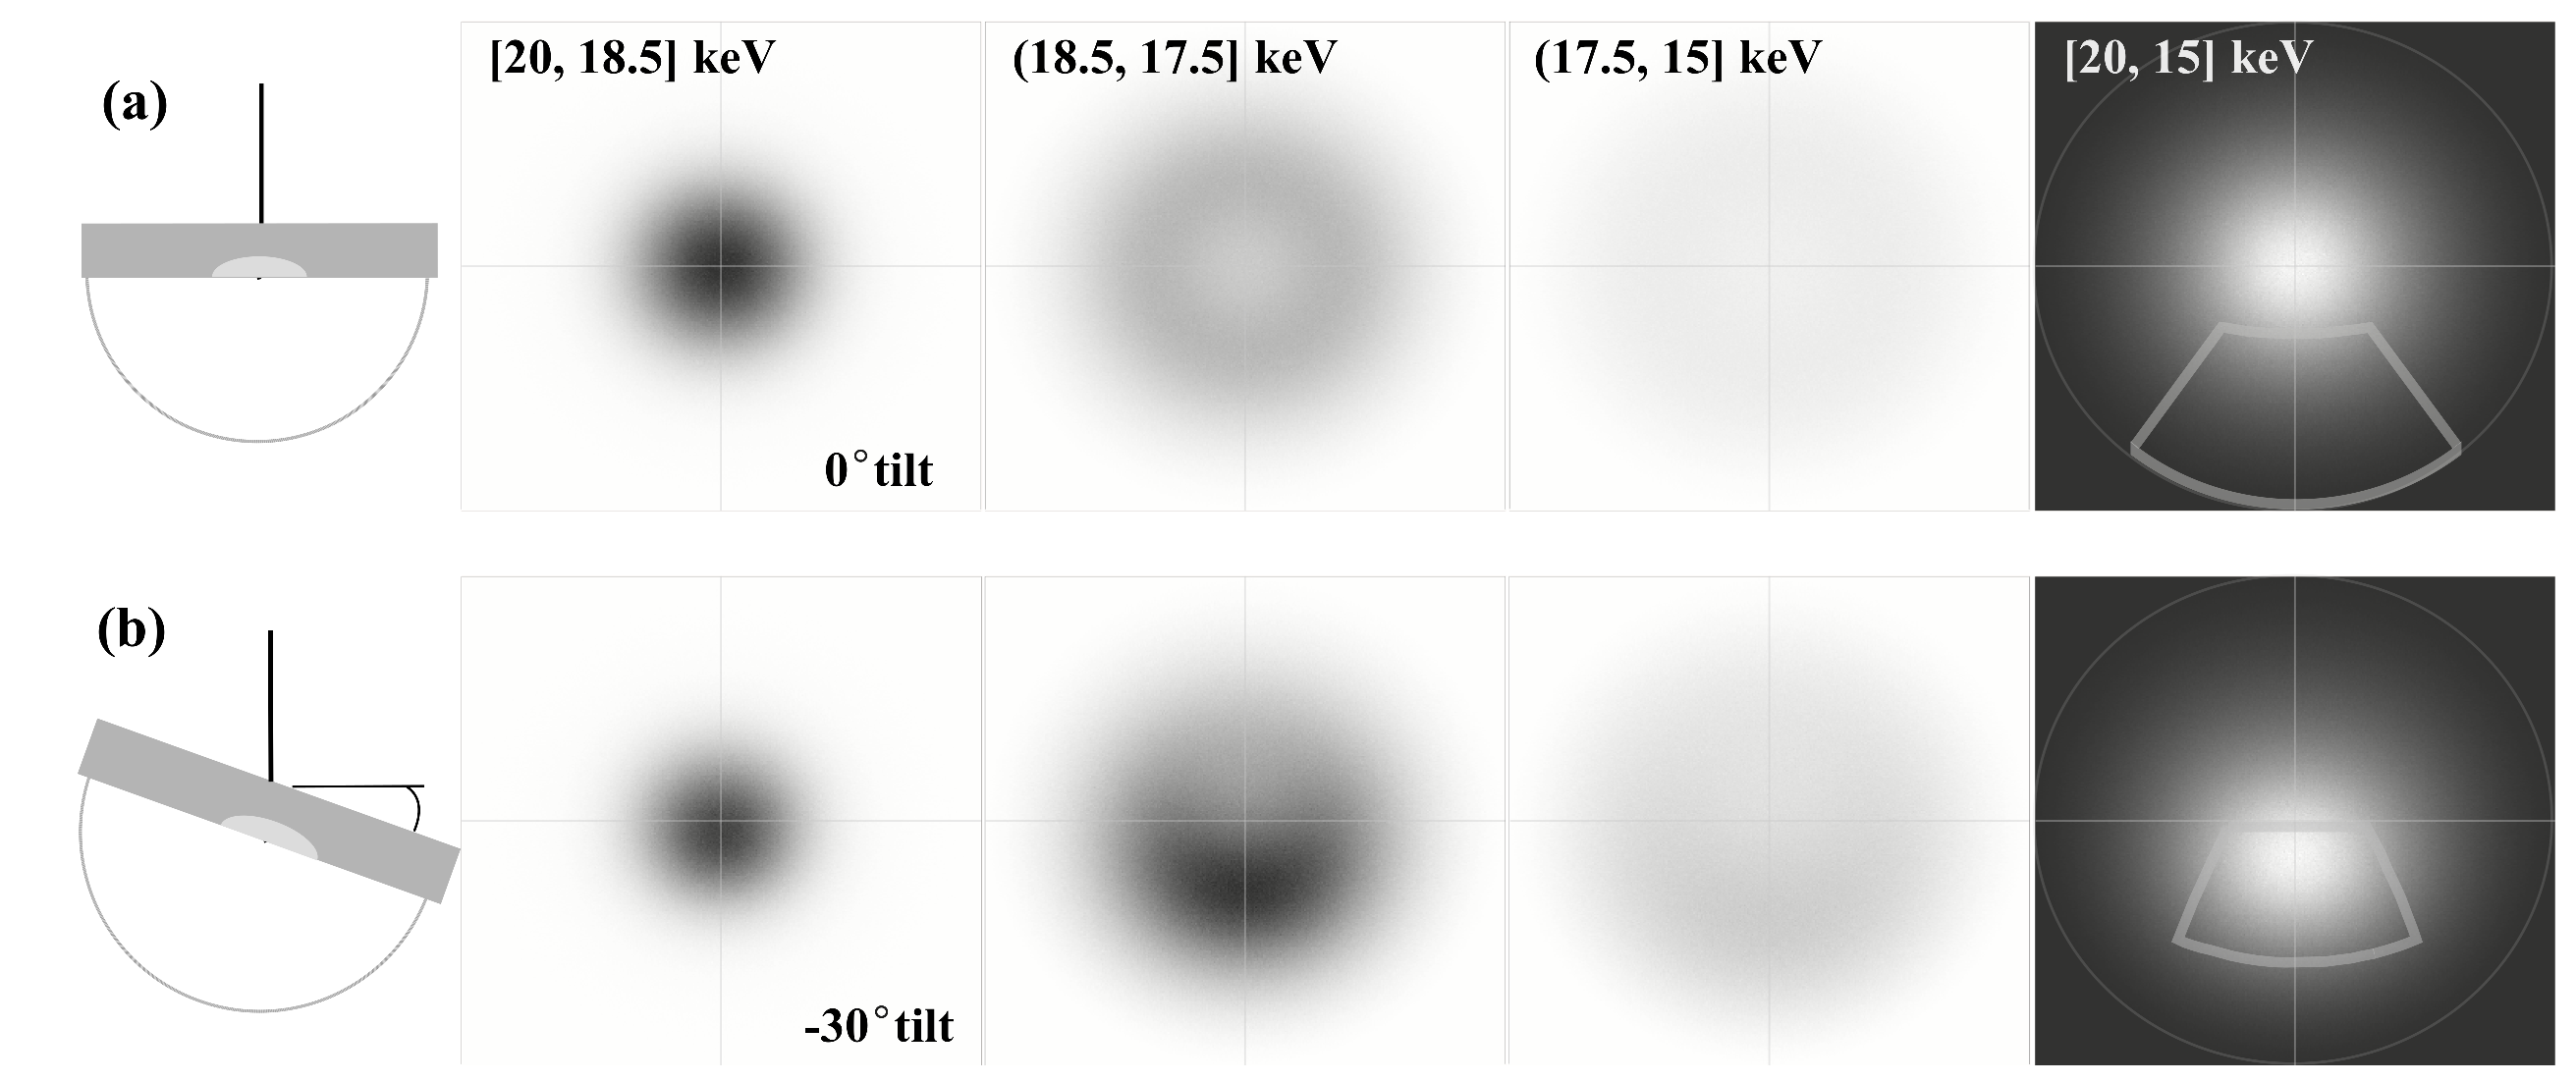
\includegraphics[width=6.in]{Fig1.eps} %TKD_SP_tilt.png
\caption{Directional distributions of transmitted electrons intensity in TKD geometry for two sample tilts (shown in the first column): 0$^{\circ}$~(a) and -30$^{\circ}$~(b). The intensities are shown here as stereographic projections where the intersection of the horizontal and vertical lines indicate the middle of the space (vertical line is the semicircle in the sketch). The first three images in each case are showing  ``energy filtered" electron intensities (reversed contrast) while the last column displays the total intensity distribution. } 
\label{fig:SP_TKD}
\end{figure}


Fig.~\ref{fig:SP_TKD} (a) shows projections for the case when the sample is horizontal and the electron beam normal. Here we can observe, as expected, that higher energy transmitted electrons are much more focused in the middle of the southern hemisphere, which happens to coincide with the direction of the incident beam. With increased energy loss we can observe an increase in trajectory randomisation or diffuseness. This can be explained by considering the possible trajectories of electrons inside the sample and their corresponding energy loss. Electrons escaping the sample with energies close to the incident beam will not have deviated far from the incident direction. Relative to this, high loss electrons are more likely to escape at large angles to their incident direction. Very high energy loss electrons appear to have no preferred escape direction and we can expect these electrons to only contribute to image background (FSE2). 

In Fig.~\ref{fig:SP_TKD} (b) we investigate the effect of tilting the sample on the angular distribution of exiting electrons from the bottom surface. Similarly, the high energy electrons will not deviate far from their incident trajectories. However, in this case, the incident direction does not correspond to the centre of the SP space and we observe that the directional distribution of the low loss electrons clusters  $30^{\circ}$ below the SP horizon. The trajectories of higher loss electrons start to be randomised in the entire SP space. We can also observe in these images how the radial symmetry of electron scattering is broken by the tilt angle of the sample. Finally, the angular distribution of the highest loss electron distribution will look the same as for the flat sample as their ``memory" of the incident direction is lost.


The outline in the rightmost column of Fig.~\ref{fig:SP_TKD} (a) and (b) depicts a typical detector projected onto the stereographic disk.  The detector has dimensions $24\times 36$ mm$^2$ and is inclined by $10^{\circ}$ from the vertical direction.  The perpendicular distance from the exit point on the bottom of the sample to the detector is $20$ mm, and the top edge of the detector lies in the sample plane for the $0^{\circ}$ orientation.  The detector bottom is closest to the centre of the stereographic projection.  For $0^{\circ}$ sample tilt, most of the scattered electrons miss the detector surface; for a $-30^{\circ}$ sample tilt, the intensity maximum moves upwards onto the lower part of the detector and at the same time the detector projection moves closer to the centre of the stereographic disk, indicating that a significantly larger number of electrons will reach the scintillator.  It should also be noted that a typical raw TKD pattern will display a rather steep intensity gradient from top to bottom, in agreement with the intensity distribution inside the detector outline in Fig.~\ref{fig:SP_TKD} (b) (rightmost image).


It becomes apparent that the sample geometry constitutes an important parameter in the formation of the Kikuchi patterns. Similarly to the EBSD case, where the sample tilt determines the preferred trajectories of electrons of different energies scattering back from the sample~\cite{degraef2013e}, the tilt of the thin film in TKD will directly influence the angular distribution of transmitted electrons suffering diffraction at different energies. In the following section we will carefully review the effect of another system parameter, the sample thickness, on the TKD diffraction patterns. 
 
%
\subsection{Sample Thickness in TKD}
\label{sec:TKDthickness}
While for the EBSD and ECP modalities one only needs to run a single Monte Carlo simulation to obtain the energy-depth-direction histogram $\bar{\lambda}_{\mathbf{k}}(E,t)$ for a bulk sample, for the TKD case, the MC simulation results depend on the thickness, $t$, of the sample.
The larger the thickness, the more energy an electron will lose on its way to the exit surface, and this will shift the entire exit energy distribution to lower energies for increasing sample thickness. 


\begin{figure}[ht]
\centering\leavevmode
\includegraphics[width=6.2in]{Fig2.eps}%{Energy_depth_KDE.png}
\caption{\label{fig:E_z_KDE}KDE plots of electron energy versus escape distance distributions as predicted by the MC model for TKD geometry for two sample thicknesses (a) 100 nm and (b) 200 nm. The area enclosed by the thick line contains 90$\%$ of events. See text for further details. }
\end{figure}

This behaviour is shown in Fig.~\ref{fig:E_z_KDE} as kernel density estimate (KDE) distributions~\cite{KDE} of electron escape energy versus escape distance predicted information for two different Ni thin foil thicknesses, 100 nm and 200 nm respectively, in the TKD geometry. Darker colours show that more electrons are likely to escape the sample with the corresponding parameters. The likelihood intensity across the two images has been normalised to the maximum value in Fig.~\ref{fig:E_z_KDE} (a) such that the intensity across images can be compared. We also show the escape energy and distance region where 90$\%$ of electrons are expected to come from, which is indicated by the thick line. Comparing the two figures, \ref{fig:E_z_KDE}(a) and \ref{fig:E_z_KDE} (b), it is clear that the thickness of the thin sample strongly influences the shape of the distributions. Considering the y-axis, the energy range of the electrons exiting the sample broadens and the energy decreases to significantly lower values as the thickness of the film increases. These observations already indicate that we should expect more diffuse diffraction patterns from thicker samples when compared to thinner ones. In general, the greater the interaction volume of electrons with the sample, the more energy will be lost by electrons before diffraction and the greater the diffuseness of the Kikuchi patterns; as supported by literature~\cite{rice2014}. 

Considering the $x$-axis, we observe that the escape depth profile resembles the usual power-law distribution~\cite{winkelmann2016} with the bulk of the electrons carrying diffraction information originating from a few nm below the escape surface. It should be noted, that the MC model used in this study does not aim to predict the full depth of diffracting electrons or interaction volume. Instead, we make the assumption that the mean value of the full diffraction depth distribution can be estimated to be of the same order as the electron mean free path. Due to the power-law distribution rule, we can be confident that the vast majority of escape depths is considered in this model.

By comparing the two images in Fig.~\ref{fig:E_z_KDE}, it should be clear that accounting for the effect of sample thickness is essential when predicting accurate electron transmission diffraction patterns. In this model this is achieved by sampling the above likelihood distribution bin-wise and constructing the $\bar{\lambda}_{\mathbf{k}}(E,z)$ weighting function as discussed in Section~\ref{sec:energy_weight}.

In the next section, we will investigate special geometries for which electrons reaching different regions of the detector can be described by the same $\lambda_{\hat{\mathbf{k}}}(E,t)$ function, simplifying the calculations significantly. 



%
\subsection{Special Sample-Detector Geometries and the Master Pattern}
\label{sec:geom}


\begin{figure}[t]
\centering\leavevmode
\includegraphics[width=4in]{Fig3.eps}%{detector_EP.png}
\caption[EBSD, TKD and ECP setup geometries]{(a) and (b) EBSD geometry, with the sample inclined at $70^{\circ}$ and $50^{\circ}$; the detector is indicated by a thick line and is inclined by $10^{\circ}$ with respect to the vertical direction. (c) and (d) show typical TKD geometries with a horizontal sample, and one inclined at $-20^{\circ}$.  Different $\mathbf{k}$ directions are indicated for which energy-distance KDEs distributions are shown in Figure~\ref{fig:ks}. (e) and (f) show typical ECP geometries with two different sample tilt angles.}
\label{fig:geometries}
\end{figure}


Consider the sample and detector geometries shown in Fig.~\ref{fig:geometries}(a-f) where the lighter region on the samples depicts the volume in which electrons suffer scatter events. The top row shows two potential EBSD geometries, one with the sample tilted at the standard $70^{\circ}$ angle with respect to the horizontal plane, the other with the sample tilted at $50^{\circ}$. As previously discussed, the sample geometry will determine the manner in which the scattering radial symmetry will be broken. Nevertheless, the region of SP space sampled by the position of the detector will also influence the uniformity (or lack thereof) of the electron energies and diffraction distances distributions. In Fig.~\ref{fig:geometries}(a), the electrons that reach the top and bottom of the detector (thick line on the left, inclined at $10^{\circ}$ from vertical) ought to have travelled approximately the same length inside the sample before channelling out; in Fig.~\ref{fig:geometries}(b) on the other hand, the electrons that reach the bottom of the detector have travelled a significantly larger distance inside the sample. 

\begin{figure}[t]
\centering\leavevmode
\includegraphics[width=6.2in]{Fig4.eps}%{ks_KDEs.png}
\caption{KDE plots of electron energy versus escape distance distributions as predicted by the Monte Carlo model for TKD geometries and directions $\mathbf{k_i}$ shown in Figure~\ref{fig:geometries}(c) and (d). The area enclosed by the thick line contains 90$\%$ of the events.}
\label{fig:ks}
\end{figure}

In TKD, the situation is similar: in Fig.~\ref{fig:geometries}(c) the sample is horizontal and electrons that reach the top of the detector have travelled a much larger distance inside the sample before diffracting than electrons that reach the bottom. In the top row of Fig.~\ref{fig:ks}, the escape energy-escape distance distributions are shown as KDE plots for electrons reaching the top (a) and the bottom (b) of the detector. We can observe qualitative differences in these distributions, especially for the escape energies. The electrons that travelled larger distances before diffracted lost more energy and therefore their energy distribution is shifted towards lower values. On the other hand, a small sample tilt of $-30^{\circ}$ shown in (d) reduces these differences. Fig.~\ref{fig:ks} (bottom row) shows that the energy-distance distribution of electrons reaching the top of the detector (c) and the distribution of those reaching the bottom of the detector (d) is qualitatively the same. Note that figures~\ref{fig:ks} (b), (c) and (d) show similar distributions since all possible trajectories $\mathbf{k_2}$, $\mathbf{k_3}$, $\mathbf{k_4}$ have similar lengths in the sample.


Finally, for the ECP case illustrated in Fig.~\ref{fig:geometries}(e) and (f), a small sample tilt does not significantly change the distribution of path lengths inside the sample, and most trajectories have about the same path length.


This observation has consequences for the numerical approach to be used to obtain high quality simulated patterns. For special geometries, we can now approximate the weighting function $\bar{\lambda}$ by an effective (averaged) weighting function,
\begin{equation}
    \bar{\lambda}_{\hat{\mathbf{k}}}(E,t) \rightarrow \bar{\lambda}(E,t),
\end{equation}
which no longer depends on the electron direction $\mathbf{k}$.  This has significant advantages numerically, since one can now pre-compute the probabilities $P(\mathbf{k})$ for a spherical sampling of incident beam orientations and store the resulting BSE yields in a master pattern (MP) that can be used to generate individual EBSD/TKD patterns by means of bi-linear interpolation, a fast and efficient way to compute many patterns in a short amount of time.  

For EBSD and TKD simulations and sample orientations that deviate significantly from the standard orientations, one can not apply the above approximation, since the range of distances travelled inside the sample is quite broad; thus, in these cases one must carry out the integrations of Equation~\ref{eq:Pn} for each individual EBSD/TKD pattern, which results in a slow computational tool.

For ECPs, the situation is quite different, since only BSE1 electrons carry coherent diffraction information; all other (BSE2) electrons only contribute to the background intensity.  A BSE1 electron has nearly the same exit energy as the incident electron since the Rutherford backscatter event is the first major scattering event after entering the sample.  Therefore, nearly all BSE1 electrons have the same exit energy and the energy integration can be eliminated, leading to the following expression which is valid for the ECP case only (with $E_0$ the incident electron energy):
\begin{equation}
    P_n^{\text{ECP}}(\hat{\mathbf{k}}) = \sum_{j\in \mathcal{S}_n}\sigma_j
    \int_0^{t_0(E_0)}\!\!\!\!\!\!\mathrm{d}t\, \bar{\lambda}(t)\vert\Psi_{\hat{\mathbf{k}}}(\mathbf{r}_j;E_0,t)\vert^2,\quad\text{with}\quad  \bar{\lambda}(t) \equiv \frac{\lambda(z)}{N t_0(E_0)}.\label{eq:PnECP}
\end{equation}
Therefore, the master pattern approach is quite well suited for the ECP case as well. For standard geometry EBSD/TKD patterns and ECPs the master pattern is computed only once for a given crystal structure and microscope voltage, and can be used to compute individual patterns by interpolation.  

TKD master pattern simulations proceed along lines similar to the previously published EBSD \cite{degraef2013e} and ECP \cite{degraef2017k} modelling approaches. A uniform grid of points is generated on a spherical surface surrounding a hypothetical spherical crystal located at the centre; each sampling point represents one outgoing beam direction $\mathbf{k}$, and the radius of the sphere is the maximum integration depth $t_0(E)$.  The sampling scheme employs the modified Lambert projection introduced in \cite{rosca2010a,degraef2013e} in which a uniform grid on a square is mapped onto the sphere by means of an equal-area projection. For each beam direction, and for a given sample thickness, one carries out the integrals of equation~\ref{eq:Pn}, using the Monte Carlo $\lambda(E,t)$ weighting function determined for that sample thickness.  In the following section, we show example TKD master patterns and compare them to similar patterns for the EBSD and ECP modalities.



\section{Results\label{sec:results}}

\subsection{Comparison between EBSD, ECP, and TKD master patterns}
\label{sec:comparison}
The master pattern expression in Eq.~\ref{eq:Pn} reveals that EBSD, ECP, and TKD master patterns have a lot in common; in particular, the dynamical scattering process that underlies the generation of Kikuchi bands is identical for the three diffraction modalities. The only differences occur in the directional, depth, and energy distributions of the B/FSEs that contribute to the patterns.  To illustrate the similarity of the master patterns, Fig.~\ref{fig:MPs} shows a portion of the upper right quadrant (centred on the $[111]$ pole) of the energy-weighted silicon master patterns for (a) ECP, (b) and (c) TKD for two different foil thicknesses ($50$ and $250$ nm) and (d) EBSD. The  microscope voltage is $20$ kV for all patterns, with a specimen tilt angle of $70^{\circ}$ for EBSD, $0^{\circ}$ for ECP, and $-20^{\circ}$ for TKD.  The patterns are very similar but differ in small details. The TKD master patterns are plotted with added colour in order to highlight  subtle differences.

\begin{figure}[t]
\centering\leavevmode
\includegraphics[width=6in]{Fig5.pdf}%{MP.png}
\caption{Portion of the stereographic projection, centred on the $[111]$ pole, of a master pattern for silicon for (a) ECP, (b) and  (c) TKD for sample thicknesses of $50$ and $250$ nm and (d) EBSD. The profiles in (e) represent the intensity along the central line (marked as a dashed line in (a)), for all four cases; the profiles have been offset vertically to make them more visible. The energy loss distribution estimated by the MC model for all four cases is shown in (f) as Poisson distribution fitted curves. }
\label{fig:MPs}
\end{figure}

Fig.~\ref{fig:MPs}(e) shows line scans through each of the master patterns, slightly vertically offset to make the profiles more clearly visible. The differences in details across the patterns is seen here distinctly. The scan across the ECP pattern in Fig.~\ref{fig:MPs}(a) displays significantly better resolved peaks compared to the EBSD one Fig.~\ref{fig:MPs}(d), supporting the better resolution observed in the ECP master pattern. Since the main signal in the ECP case consists of BSE1 electrons which have lost only a small amount of energy in the sample before being backscattered, one can consider ECPs to be energy-filtered versions of EBSPs.


The line scans across the TKD patterns for different thickness films are more similar to each other, except for the shift in peaks in the zone axis (highlighted by the grey box). It is rather apparent that both the peak positions and the sharpness of the thin film (50~nm) TKD pattern are more similar to the ECP pattern, while the peaks and blurriness of the thick film TKD pattern are closer to those of the EBSPs. We explain this behaviour by considering the energy loss of electrons contributing to the patterns in each case. The Monte Carlo predicted energy loss spectra for all four cases described above are shown in Fig.~\ref{fig:MPs}(f) as fitted Poisson distribution curves. Thin film TKD patterns are produced by electrons with an energy range very close to the ECP case. Similarly, increasing the sample thickness causes the electron exit energy distribution to become wider and shift to lower energies, which corresponds to a broadening and slight blurring of the Kikuchi bands due to the increased Bragg angles; these phenomena are common to EBSPs and thick films TKD patterns. 


It becomes apparent that the sample thickness can be seen as an energy filtering mechanism in TKD. In terms of the traditional Hough-based indexing approach, one must thus select a butterfly mask of the appropriate width, depending on the sample thickness and incident electron energy. For the dictionary indexing approach, illustrated in section~\ref{sec:DI}, the pattern dictionary must be computed using the appropriate Monte Carlo and master pattern data, to ensure accurate matches between experimental and simulated patterns.



The EBSD master pattern is an energy-weighted average of individual master patterns and the integration over the electron energy gives rise to a continuous range of Bragg angles and, thus, a general blurring of the master pattern features compared to the ECP case. This will also be the case for individual diffraction patterns that are extracted from the master patterns via bilinear interpolation, as explained in \cite{degraef2013e}.

\subsection{Comparison with Experimental Patterns\label{sec:compexp}}

Fig.~\ref{fig:TKDpatternfit} shows two experimental TKD patterns (left column) for a nano-crystalline Aluminum sample, acquired at $30$ kV with a sample tilt of $-18^{\circ}$ in a FEI Teneo field emission scanning electron microscope, using the TSL Hikari EBSD detector system; the sample foil is approximately $150$ nm thick.  Monte Carlo and master pattern simulations were carried out for these parameters.  The detector parameters and grain orientations were obtained through an in-house developed interactive fitting routine, written in the Interactive Data Language \cite{IDL}; an initial approximate grain orientation is obtained by visually comparing the simulated TKD pattern with the experimental pattern.  Once a reasonable orientation is obtained, the detector parameters are refined by using a downhill simplex routine to minimise a cost function, either the normalised dot product between the two patterns or their mutual information.  When a reasonable set of parameters is obtained, the grain orientation is refined, and the process is repeated until both detector parameters and grain orientation are satisfactory.  This process was applied to the pattern in Fig.~\ref{fig:TKDpatternfit}(a), and the resulting detector and orientation parameters are listed in Table~\ref{tb:fit}.   


\begin{figure}[t]
\centering\leavevmode
\includegraphics[width=5in]{Fig6}
\caption{(left column) Experimental TKD patterns for Aluminum at $30$ keV and (right column) corresponding simulated patterns; brightness and contrast of the simulated patterns have been adjusted to better match the experimental patterns.  Simulation parameters for both (a) and (b) are stated in the text. The dot product values between normalised patterns are equal to $0.881$ for the top pair and $0.834$ for the bottom pair, indicating a satisfactory match.}
\label{fig:TKDpatternfit}
\end{figure}

The same detector parameters were then used to refine the orientation of the pattern in Fig.~\ref{fig:TKDpatternfit}(b).  The resulting simulated patterns are shown in the right column of Fig.~\ref{fig:TKDpatternfit}.  Note that the only adjustments to the simulated patterns were brightness and contrast changes to maximise the visual agreement between the simulated and experimental patterns.  The overall intensity gradient (from bright at the bottom of the pattern to dark at the top) follows directly from the use of the direction-dependent Monte Carlo statistical data, and is in good agreement with the intensity gradients of the experimental patterns.  The satisfactory agreement between simulated and experimental patterns indicates that the energy-weighted dynamical scattering model employed in the pattern simulations is sufficient to obtain realistic pattern simulations. 




%
\section{Discussion and Conclusions \label{sec:discussion}}

Inelastic scattering, a phenomenon usually discarded in diffraction simulations, has direct influence on the energy distribution of diffracting electrons and, consequently, on the imaged Kikuchi patterns. The broader the energy distribution of diffracting electrons, the more diffuse the Kikuchi band edges. Using a Monte Carlo model we can observe that the length of electron trajectories before diffraction is a determining factor in the broadening of the energy distribution. This factor, in turn, can be controlled in the Transmission Kikuchi Diffraction modality through the thickness of the sample, acting effectively as an energy-filtering mechanism. Another determining factor for the energy distribution is the sample-detector geometry which influences both TKD and EBSD modalities.



We should note that the Monte Carlo model used in this work explicitly describes the lower escape distance values for the signal carrying electrons.  A subset of electrons reaching the detector will, nevertheless, carry a probability of channelling over longer trajectories. Depending on their travel direction inside the crystal, these electrons are expected to give rise to contrast inversion of one or more Kikuchi bands (observed as dark instead of bright lines). This will occur when the distance travelled is of the order of, or larger than, the extinction distance for a particular plane. Contrast inversions are thus expected to occur for both EBSD and TKD modalities when the sample is tilted such that long electron trajectories are possible; in addition, the sample should have a crystal structure that gives rise to short extinction distances. For the ECP modality, contrast inversions are not expected to occur unless very large sample tilt angles are used, which is not practical due to the possibility of the sample hitting the back-scatter detector. Similarly, when the TKD detector if mounted horizontally, below the sample, the electron trajectories inside the sample will have a narrow range of escape distances, so that contrast inversions are also not expected to occur. A statistical model more sensitive to the outlier cases of long distance channelling electrons is therefore necessary if we are to correctly predict band contrast inversion. 

The energy-weighted scattering model is shown to correctly predict Kikuchi bands sharpness (defined as signal to noise intensity) for the different SEM modalities. When used for the dictionary indexing approach it was shown to produce indexed TKD patterns with fewer incorrectly indexed points compared to commercial Hoigh transform based indexing software. 
 
\chapter{Summary, discussion and further work}
\label{chap:Conclusion}


I believe I have learned a good deal of facts and skills during my PhD programme. I think that because I'm somewhat confident that re-deriving the results shown here with the knowledge of today, would only take me a fraction of the four years period; possible famous last words. Having therefore great value for me, I wanted to have this knowledge written down in as much detail as this format would afford. The result is the textbook style of the first two chapters. 

My experience from the inside of the ivory tower that is academia is that there is no such thing as a unified consciousness of science, if a fact is understood in a certain field, the knowledge doesn't automatically carry in another, and sometimes the same science must be re-learned fifty years later because there was no bridge (research funds) to carry the wisdom; defying altogether the naive perception of science I gained as an undergrad. I dedicated multiple pages in this document, then, not to ground-breaking new science, but to knowledge that ought to be more within reach to the average scientist dedicated to diffraction in the SEM. I also dedicated more time than I would like to admit to describing the crystallography of the wurtzite system, including a full appendix of point group theory. The later was admittedly mostly for myself, but it would be nice to see more often the correct crystallographic unit cell of wurtzite (and not the hcp one) in talks about diffraction. 

In Chapter~\ref{Chap:Diffraction} I covered  everything electron diffraction, including describing where the values of important diffraction parameters, like the structure factor, come from.  I also took it upon myself to show graphs for scattering factors for group-III nitride systems (AlN, GaN and InN) and explain the insights they provide. Not only intuitive ones like the fact that the atoms in AlN will elastically scatter fewer electrons and, therefore, give a poorer signal to noise when it comes to ECC imaging, but also less intuitive aspects, such as families of planes that are more densely packed (such as the \textit{a}-plane) scatter fewer electrons then their less packed counterparts (such as \textit{c}-plane). This is somewhat unfortunate for the study of \hkl[001] wurtzite nitrides in the forward scatter geometry in the SEM. 

I then go on to talk about the wurtzite structure factor in these systems and comment on their predictions, including the failure of Friedel's law for non-centrosymmetric systems and the systematic absences we can expect. Embarked with all these information I spend the rest of the chapter applying the Howie-Whelan dynamical model to the ECCI geometry. I make the argument the equations should still hold even if we replace the dependence on depth in the sample of the Bloch waves with that on the distance travelled by the primary beam.  

Having the two beam dynamical equations laid out, in Chapter~\ref{chap:ECCI} I go over adding the displacement field introduced by a threading dislocation and using this model to predict the observed dislocation associated contrast in ECCI which I call \textit{ECC-strain}. I spend some effort emphasising the importance of setting out the correct reference frame transformations. In the  end, I argue, the contrast profile of a dislocation observed in ECCI is nothing more than a map of the strain projection selected by the diffraction conditions. Having worked out the complex relationship between the many frames involved, looking at the physics predicted by the strain profile of dislocations becomes a piece of cake.  

For instance, I show how the sample tilt affects dramatically the surface relaxation of the ECC-strain and that, in turn, will enhance the contrast. I then interrogate the ECC-strain for forward model geometry about whether the diffraction condition or the Burger vector dominates the contrast profile. I conclude that edge TDs ECCI contrast profile generally follows the Burger vector while the diffraction condition mostly affects its magnitude. I also compare these predictions with   experimental data to confirm the behaviour.


All this analysis was done for a two beam dynamical model. This approach is a valid prediction of a strong two beam diffraction condition. This, in turn, is a likely condition to achieve for SEM electron energies which describe a smaller Ewald sphere, which will likely intersect a few reciprocal lattice points, as opposed to the large sphere the TEM electron energies correspond to. It would be interesting in future work, as already suggested by Prof. De Graef, to compare the two beam model prediction to the multi-beam one and assess how correct these assumptions are. 

For a fact, I suspect that the strong beam is not always fulfilled in ECC images. It is my inkling that, in fact, ECC images showing only bright intensity at dislocation positions, mostly in metals, \eg steel~\cite{Gutierrez09} or Al~\cite{Barnoush10}, are obtained closer to weak beam conditions where the deviation from the Bragg angle, $\mathbf{s}_g$ is large. In this case, instead of bright-dark contrast, the dislocation moves locally the reciprocal lattice point closer to the Ewald sphere, showing as higher diffracted intensity on the micrograph. This is an interesting case especially because the Laue geometry approximation will become less feasible. To my knowledge, literature is yet to address the physics and possible models of predictions for, what is a common representation of ECCI, high intensity at dislocation positions in the SEM. 

The fact of the matter is that ECCI models are nowhere near mature and here are two more points that I can think of where they are lacking. In terms of the TD displacement predictions, I approximated the anisotropy of wurtzite system to an isotropic one plus corrections. It would be more accurate to consider full anisotropy and models for that exist~\cite{Barnett71}. But this would make a small difference  compared to introducing grains in the continuum model~\cite{Read50}. Dislocations on grain boundaries are ought to introduce a very different displacement field that is incomparable to that introduced by dislocations in a true continuous medium~\cite{Van02}. And we know plenty of dislocations lie on the grain boundaries. Grain boundaries facilitate dislocation pile-ups and influence directly the hardness of a material. Since TEM requires sample to be as thin as the size scale of grains, the sample preparation will introduce relaxation that will affect the grain structure. ECCI is therefore the only possible non-invasive imaging technique of dislocations at boundaries. Unfortunately, due to the limited number of  investigations we don't yet know how to use it precisely.

The other point of improvement is related to the Monte Carlo discussion in Chapter~\ref{chap:TKD}. I approximate the incident coherent beam penetration depth using Monte Carlo models that do not take into account diffraction whatsoever. I use the escape depth of low loss electrons, but the model does not know that diffracting electrons suffer less inelastic scattering and can travel further. Since the values I obtain are on the same scale as the literature offers, I think the values should be in the right ballpark, but it would be a worthwhile effort to quantitative study of how deep in the sample the ECC signal comes from.

Chapter~\ref{chap:TKD} discusses the importance of taking into account multiple electron energies when modelling EBSD/TKD patterns. It shows that for the TKD geometry, the low side of the energy distribution of the low loss electrons contributing to the Kikuchi patterns will be highly anisotropic on the detector. In other words, not taking into account an energy distribution for the low loss electrons will fail to predict not only the intensity distribution along the Kikuchi lines, but also the their width variation as well as details.

We also show how the sample thickness acts in effect as an energy filtering mechanism for the diffracting electrons in TKD. In terms of comparing the Kikuchi patterns in all the diffraction mechanism in the SEM discussed in this Thesis, Fig.~\ref{fig:MPs} on page~\pageref{fig:MPs} is an insightful one. Comparing the energy distribution of electrons contributing to ECP, TKD and EBSD patterns, and with it the resulting sharpness and details of the simulated Kikuchi lines on the MP, we conclude that the TKD modality is bridging the gap between the very narrow energy window of the ECPs and the broader energy range of EBSD. 


\section{Epilogue -- Science as an incremental, open process}

The history of science is all too often taught as a chronological list of discoveries. There is undeniable value in this approach as it reflects the arrow of complexity of notions. However, it leads to a very simplified image of the development of scientific knowledge: one big idea bringing over the next and so on. On page~\pageref{table:historyDiff}, I too show the history of diffraction as a table of chronological events. These are big shift events, which radically and permanently changed the way future science was to be done in this area. A good number of names in this table were awarded for their significant contribution with Nobel prizes. Nevertheless, the table is clearly a gross simplification of history, omitting, due to lack of space, the incremental refinement and maintenance work that supported and propelled the bigger ideas. It is quite common for important work of individual voices to be wiped away from science history as we associate a breakthrough to a single name or even to a small group of people. Seeing the bigger picture is, undeniably, worthwhile, but we must not mistake it for the full picture.

The ``unremarkable'' work done by the rest of the community, not awarded prestigious prizes, is not less important for the advancement of science. Quite the opposite. Neither science nor culture truly advance in big steps. In a recent study published in Nature, Miu \etal~\cite{Miu2018} looked at the way pieces of software get improved by a community of developers in a simulation of cumulative cultural evolution. One of the observations was that the vast majority of advances are of an incremental type and not, as the scientific community expect, leaps in knowledge. Observing the strong positive breakthrough bias of scientific publishing, one would find it hard to assume that enough credit is given to the ``tweakers''. 

Another critical observation was that big changes in the paradigm are more likely to turn out unsuccessful than smaller tweaks. Remember the Nobel prize in medicine awarded for the ``discovery'' of brain lobotomies\footnote{ ``for his discovery of the therapeutic value of leucotomy in certain psychoses''-- The Nobel Prize in Physiology or Medicine 1949~\cite{Nobel49}.}? Thankfully, neuroscience moved away from this particular scientific breakthrough. And it did that with small, incremental improvements on the understanding of the brain. Any sort of conversation about the development of science focused only on the leaps of knowledge must ultimately be misrepresenting the scientific process.


In this paradigm of scientific value misrepresentation, scientific code suffers perhaps even more. The philosopher Daniel C. Dennett, in his latest book \textit{From bacteria to Bach and back}~\cite{Dennett} makes the case that evolution is not only a good protocol for developing fit biological organisms but can, in fact, be successfully applied to a variety of concepts, perhaps, he argues, consciousness, the human mind and even code development. The latter analogy I find compelling. Similarly to adaptable organism having emerged from surviving a variety of conditions, the power of good code stands in the number of iterations it went through. Of course, we cannot wait around for functional code to ``occur'' as the results of tens of millions of years of iterations, and, after all, we expect developers to be somewhat wiser than the random processes occurring in nature. Nevertheless, in the end, each iterative step has the chance to rectify errors or limitations in the code, weed out unnecessary/old lines and replace them with new, more optimised, features. Established software tends to be software reviewed by many pairs of eyes. Yet, scientific software continues to be developed and  maintained by small groups and destined to see the light of only a handful of iterations.  


To add insult to injury, scientific code is rarely developed to be open and even more rarely made easily accessible. Here is another example of anecdotal evidence of why I think this a counter-intuitive way of following the scientific method. Two condensed matter groups set out, independently, to predict the behaviour of supercooled water, and, even though they implemented the same method, their results contradicted each other for seven straight years~\cite{supercool}. During this time, while the groups were in contact with one another, the actual lines of code never changed hands. When it finally did, a bug was discovered by the ``competing'' team in just a few months. I'm pointing out that we could have known in a few months, not seven long years, that water is predicted to change phase when supercooled. When scientific groups working in the same field do not collaborate with each other for whatever reason, it is science that suffers.


In the light of all these, I want my thesis work to make a positive tweak in the endeavour of making electron diffraction in the SEM a well-understood phenomena in the electron microscopy community. I aim for this work to aid the understanding of why we can observe and how we can study dislocations in the SEM and I do not expect it to be the definitive attempt. For these reasons I tried to make this document as accessible as possible for whoever wants to continue on this journey. I tried to explain in depth the building blocks I used and why I chose them, I provide access to whatever code I ran or wrote and I offer a small collection of extra materials. May your code and science be even a little bit better than mine!
%

%----------------------------------------------------------------------------------------
%	THESIS CONTENT - APPENDICES
%----------------------------------------------------------------------------------------

\appendix % Cue to tell LaTeX that the following "chapters" are Appendices

% Include the appendices of the thesis as separate files from the Appendices folder
% Uncomment the lines as you write the Appendices

\chapter{Implementations}

I refer throughout this document to supplementary pieces of code, most in \emph{Python} and some in \emph{Fortran95}. I tried to describe in detail what they do, sometimes I included pseudocode and other times I just statet the relevant equations. They can all be found on my, otherwise rather pristine, public GitHub repository~\cite{myGitHub}. 

The Python scripts have been written in Python 2 which can be easily installed on Ubuntu machines (or most Linux flavours) from the package manager or by typing in 18.04 or later:
\begin{verbatim}
$ apt install python-minimal
\end{verbatim}

Files containing Python script can be easily recognised from the \textit{.py} file type and can be run with with:
\begin{verbatim}
$ python filename.py
\end{verbatim}

To run Fortran code on a Ubuntu machine  use the gfortran compiler, which again can be found in the package manager or can be installed via:
\begin{verbatim}
$ apt install gfortran
\end{verbatim}

For the Fortran files I wrote a \textit{Makefile} that compiles the dependencies in the correct order. It can be run by simply typing $make$ in the command line. Once everything is compiled it iss just a matter of running the executable. 

For the smaller scripts I use \href{http://jupyter.org}{\texttt{Jupyter}}~\cite{Jupyter} notebooks written in Python. I will assume the reader has Python 2.7 or greater installed. The \href{https://anaconda.org/}{\texttt{Anaconda}} Python distribution~\cite{Conda} ships with Jupyter among other packages useful for scientific computation. However, if you have Python already installed then you can use the package manager \href{https://pypi.org/project/pip/}{\texttt{pip}} to add new libraries:
\begin{verbatim}
$ pip install jupyter
\end{verbatim}
To start a Jupyter notebook kernel you just type:
\begin{verbatim}
$ jupyter notebook
\end{verbatim}
And navigate to the desired script file. Individual cells are compiled with \texttt{Shift} + \texttt{Enter}.

In some notebooks I use the \href{https://plot.ly/}{\texttt{plotly}} package ~\cite{Plotly} for plotting. These figures are interactive but do require an account on the \href{https://plot.ly/}{\texttt{plotly} website}\footnote{ \texttt{Plotly} website url is \href{https://plot.ly/}{https://plot.ly/}.}.  

In Chapter~\ref{chap:TKD} I talk about the open software implementation of electron and optical microscopy models EMsoft~\cite{EMsoftpaper}, which can be found on Prof. Marc De Graef's GitHub~\cite{EMsoft} page where installation instructions are also given.
\chapter{Passive rotation matrices in the 3D Cartesian frame}
\label{Chap:rotations}

As described in the  main text, these are just the transpose of the active 3D rotations.

\vspace{0.2cm}

\noindent\begin{minipage}{0.47\textwidth}
The passive, anticlockwise rotation of a Cartesian reference frame around the axis $\mathbf{x}$ is given in the pre-multiplication matrix form as: 
\begin{equation*}
\mathcal{R}_\mathbf{x}(\theta)=\begin{pmatrix}
1 &  0           & 0 \\
0 & \cos{\theta} & \sin{\theta} \\
0 & -\sin{\theta} & \cos{\theta}
\end{pmatrix}
\label{eq:RotMat}
\end{equation*}
\end{minipage}
\begin{minipage}{0.5\textwidth}
\centering
\includegraphics[width=0.45\linewidth]{Figures/Rx.png}
\captionof*{figure}{Basic rotation around $\mathbf{x}$.}
\end{minipage}



\noindent\begin{minipage}{0.47\textwidth}
The passive, anticlockwise rotation of a Cartesian reference frame around the axis $\mathbf{y}$ is given in the pre-multiplication matrix form as: 
\begin{equation*}
\mathcal{R}_\mathbf{y}(\theta)=\begin{pmatrix}
\cos{\theta}  &  0     & -\sin{\theta} \\
0             & 1      & 0 \\
\sin{\theta} & 0      & \cos{\theta}
\end{pmatrix}
\end{equation*}
\end{minipage}
\begin{minipage}{0.5\textwidth}
\centering
\includegraphics[width=0.45\linewidth]{Figures/Ry.png}
\captionof*{figure}{Basic rotation around $\mathbf{y}$.}
\end{minipage}



\noindent\begin{minipage}{0.47\textwidth}
The passive, anticlockwise rotation of a Cartesian reference frame around the axis $\mathbf{z}$ in the pre-multiplication matrix form is: 
\begin{equation*}
\mathcal{R}_\mathbf{z}(\theta)=\begin{pmatrix}
\cos{\theta} & \sin{\theta} & 0 \\
-\sin{\theta} & \cos{\theta}  & 0 \\
0            &  0            & 1
\end{pmatrix}
\end{equation*}
\end{minipage}%
\begin{minipage}{0.5\textwidth}
\centering
\includegraphics[width=0.45\linewidth]{Figures/Rz.png}
\captionof*{figure}{Basic rotation around $\mathbf{z}$.}
\end{minipage}



%%%%%%%%%%%%%%%%%%%%%%%%%%%%%%%%%%%%%%%%%%%%%%
%--------- Symmetry --------------------------
%%%%%%%%%%%%%%%%%%%%%%%%%%%%%%%%%%%%%%%%%%%%%%



\chapter{Symmetry in crystallography}
\label{Chap:Symmetry}
Many objects in nature exhibit symmetry of some sort. The human body has approximate mirror symmetry. A shamrock (the species of clover or trefoil used as the symbol of Ireland) has three-fold rotational symmetry (trefoil), and here's a bit of trivia to make you a star at the next British party, not four-fold symmetry as U.S. advertisements sometimes wrongly represents it. The reader might have noticed that the way we talk about object symmetry involves a motion action, which made upon the object would leave it unchanged. Indeed, the symmetry of an object will be defined by its \textit{symmetry operations} that map the object onto itself. While for any motion one can find an object for which this is a  symmetry motion, if we start with the object it is easy to start with these three basic actions to test its symmetry\footnote{ Assuming we are to leave the metric properties of space undisturbed, \ie no stretching, bending, twisting, which should be easy to achieve in the physical world.}:
\begin{enumerate}
\item rotate
\item reflect
\item translate
\end{enumerate}

If, after any one or a combination of 1, 2 and 3, the object looks the same as it originally looked than we talk about the object as being symmetric. There is a nuanced distinction between these operations since 1 and 3 can be physically realised and known as \textit{proper} or first kind operations. Operations that involve 2 are \textit{improper} or of second kind. Inversion is yet another improper operation that can be reduced in three dimensions to a rotation plus a reflection. 

We will see that all this can be written in mathematical form with only minor adjustments. First, operation 3 can only truly be a symmetry operator for infinite objects which are not very common in everyday life. Second, the identity operator is also introduced as symmetry operator, such that, in the mathematical sense, all objects hold at least one symmetry property. Now there's nothing stopping you from being the soul of the party.

We will spend some time exploring a subset of symmetry operations chosen such that when combined can generate the entire symmetry of a wurtzite crystal. We will follow closely the notation used in \textit{International Tables for Crystallography, Volume A}~\cite{IntTableCrysA} described in some detail on page~\pageref{chap:int}. We will use the two most common shorthand notations to write down symmetry operations: the \textit{Hermann-Mauguin notation} also known as the \textit{international notation} which is the standard one, and the \textit{Schoenflies notation} which is widely used in Physics and Chemistry. We will also show the graphical symbols for the operations discussed.


\section{Symmetry operations}
\label{chap:symOp}
The set of symmetry operations of a given object have noteworthy properties:
\begin{enumerate}
\item the application of two symmetry operations results in a third symmetry operator of that object
\item the inverse of an operation is also an operation of that object
\item all objects exhibit the identity operation
\item the associative law is valid when combining three or more operations.
\end{enumerate}
These four properties are also the group axioms and tell us that the set of symmetry operations of a given object form a mathematical group. This will come in handy in the next section. For now it is worthwhile to look at how to write these operation in mathematical form.

In the following we will explore a non-exhaustive list of symmetry operations. We choose our examples such that they are relevant for generating the wurtzite crystal structure symmetry. Note that the  basis vectors of a hexagonal lattice do not form a Cartesian frame. This means that the usual algebraic formulas used for transformation operations must be revised. We do expect the form of rotation, translation and reflection matrices to be therefore not as familiar, which is why we take the time to explore them here. 



\subsection{Operation of first kind: pure rotation}
\label{sec:pureRot}

A pure rotation is fully determined by a rotation axis and a rotation angle which is chosen to be positive in the counter-clockwise direction. The rotation axis is given as a vector \hkl[uvw] and the rotation angle is given as fraction of $2\pi$. For instance a rotation of order three or three-fold rotation is a rotation by angle $2\pi/3$. In general an $n$-fold rotation is represented by symbol \textsf{n} (\textsf{C}$_n$) and Table~\ref{Table:rotation} shows examples for three-fold and six-fold rotations together with their graphical symbols which are filled polygons with $n$ sides.
 

\begin{table}[ht]
\caption{Examples of pure rotation symbols.}
\label{Table:rotation}
\centering
\begin{tabular}{l c c c }
\toprule
\tabhead{Name} & \tabhead{Graphical} & \tabhead{Hermann-Mauguin} & \tabhead{Schoenflies} \\
\midrule
 Three-fold rotation & {\Large \cry{3}} & \textsf{3} & \textsf{C$_3$} \\
 Six-fold rotation & {\Large \cry{6}} & \textsf{6} & \textsf{C$_6$}  \\
\bottomrule
\end{tabular}
\end{table}

\begin{figure}[ht]
    \centering
\includegraphics[width=0.9\linewidth]{Figures/pureRotation.png}
\caption[Graphical representations of three-fold and six-fold pure rotations.]{Rendered 3D graphical representations of a) three-fold and b) six-fold pure rotations. The circles in the bottom right of the images represent the stereographic projections of the operators.   }
\label{Fig:pureRotation}
\end{figure}

3D representations of the rotation operator are shown in Figure~\ref{Fig:pureRotation} for rotations of order 3 in (a) and 6 in (b), respectively. The images have been rendered with the public domain software \href{https://sourceforge.net/projects/rayshade/}{\textsf{Rayshade 4.0.9} software}\footnote{ Link is \href{https://sourceforge.net/projects/rayshade/}{https://sourceforge.net/projects/rayshade/}.}. The input files I used are very closely based on the input  \href{http://som.web.cmu.edu/frames2.html}{\emph{*.ray} files}\footnote{ Link is \href{http://som.web.cmu.edu/frames2.html.}{http://som.web.cmu.edu/frames2.html.}} developed by Marc De Graef~\cite{DeGraef98} with the purpose of teaching the crystallography group symmetry\cite{teachingPointGroup}. My scripts can be found at this \href{https://github.com/elena-pascal/SEM-diffraction/tree/master/Wurtzite_symmetry/}{GitHub repository}\footnote{ Link is \href{https://github.com/elena-pascal/SEM-diffraction/tree/master/Wurtzite_symmetry}{https://github.com/elena-pascal/SEM-diffraction/tree/master/Wurtzite\_symmetry}.}. The relevant files for this example are \texttt{3FoldPureRotationPNG.ray} and \texttt{6FoldPureRotationPNG.ray} and can be compiled on a Linux machine after the installation of \textsf{Rayshade} software (and making sure \textsf{ImageMagick} is available on the machine) by typing:
\begin{verbatim}
rayshade [filePNG].ray > [filePNG].mtv
convert [filePNG].mtv  [file].png 
\end{verbatim}
where \texttt{[file]} is the name of the file used. \emph{*.mtv} files can also be converted to \emph{*.png} or \emph{*.gif} with \textsf{ImageMagick}. All the input scripts and resulting images and animated files can be found in the extra materials. To render the \emph{*.gif}s one need more patience and has to do:
\begin{verbatim}
rayshade [fileGIF].ray > [fileGIF].mtv
convert [fileGIF].mtv  [file].gif 
\end{verbatim}

The small helix object used by Marc  De Graef in these images (made up of a helical string of spheres) was chosen such that it holds no rotational symmetry. The object also exhibits handedness and its mirror reflection will look different from the original object.  Despite this, the entire system, the three objects in Fig.~\ref{Fig:pureRotation} (a) or six objects in Fig.~\ref{Fig:pureRotation} (b), looks indistinguishable from original when rotated $2\pi/3 = 120\si{\degree}$ and $2\pi/6 = 60\si{\degree}$, respectively, around the rotation axis. Similarly, a triangle prism will look the same after being rotated around the central axis by $120\si{\degree}$ and a hexagonal prism will look indistinguishable after being rotated $60\si{\degree}$, respectively.

It is common for the axis of rotation to be the third basis vector \ie parallel to the crystallographic $\mathbf{c}$-axis and, in those cases, the rotation axis to not be explicitly stated. In any other case, the rotation axis must be given, either in vector form \hkl[uvw] or as the equation of the line coinciding with the axis. The latter notation method is the one used in the \textit{International Tables for Crystallography}. As an example we can look at \textit{Symmetry operation} (2) of a hexagonal lattice point group shown in Fig.~\ref{Fig:ITC}. $3^+(0,0,z)$ is a three-fold pure rotation around the \hkl[001] direction given here in line equation form. The $^+$~sign informs us that the position of the point is elevated with respect to the drawing plane. 

A three-fold symmetry of a lattice tells us that for every ``motif'' at position $(x, y, z)$ we will find the same motif at the equivalent position $(x', y', z')$ obtained through a $120\si{\degree}$ rotation around the central axis, here $\mathbf{e_z}$.  In order to represent the rotation operation in mathematical form we must turn to rotation matrices. Unlike the somewhat intuitive form when used in an everyday orthonormal system, as seen on page~\pageref{eq:RotMat}, when derived for a general, non-orthonormal lattice the rotation matrices can become cumbersome and will obscure the symmetry (see ref.~\cite{Davenport73}). Luckily, we can avoid that by considering the passive rotation of the system instead of the active rotation of the motif. 

We want to find the rotation matrix $\mathsf{D(}\theta\mathsf{)}$ which, when applied to a set of (not necessary orthonormal) basis vectors $(\mathbf{e_x},\, \mathbf{e_y},\, \mathbf{e_z})$ rotates them once around $\mathbf{e_z}$ by an angle $\theta$ to a new configuration $(\mathbf{e'_x},\, \mathbf{e'_y},\, \mathbf{e'_z})$. This passive rotation is defined in crystallography by the right hand rule\footnote{ The right thumb points towards the direction line and the fingers indicate the positive rotation.}. It should be clear that this is equivalent to an active rotation (\ie rotating a vector defined in this basis) by the same angle anticlockwise around $\mathbf{e_z}$ when looking in the direction of $\mathbf{e_z}$. 

\vspace{0.3cm}

\noindent \begin{minipage}{0.57\textwidth}

If the set of basis vectors describes a hexagonal lattice\footnotemark \, and the angle of rotation is $120\si{\degree}$ then the matrix $\mathsf{D^{hex}(120\si{\degree})}[001] \equiv \mathsf{D^{(n)}}$ is a three-fold rotation and can be derived by geometry as shown in Fig.~\ref{Fig:3foldrot}.
\begin{equation*}
\begin{split}
\begin{pmatrix}
\vb{e'_x} & \vb{e'_y} & \vb{e'_z}
\end{pmatrix}
 & =
\begin{pmatrix}
\vb{e_y} & -\vb{e_x} -\vb{e_y} & \vb{e_z}
\end{pmatrix} \\
&=\begin{pmatrix}
\vb{e_x} & \vb{e_y} & \vb{e_z}
\end{pmatrix}
\mathsf{D^{(n)}}
\end{split}
\end{equation*}

Which completely determines the matrix $\mathsf{D^{(n)}}$ to be:

\begin{equation}
\mathsf{D ^{(n)}} = \begin{pmatrix} 
0 & -1 & 0 \\
1 & -1 & 0 \\
0 & 0 & 1 
\end{pmatrix}
\label{eq:D_n}
\end{equation}
\end{minipage}
\begin{minipage}{0.4\textwidth}
    \centering
\includegraphics[width=0.85\linewidth]{Figures/3FoldaxisRot.png}
\captionsetup{width=0.7\linewidth}
\captionof{figure}{Three-fold rotation around the third axis of a hexagonal basis set. }
\label{Fig:3foldrot}
\end{minipage}

\vspace{0.5cm}

\footnotetext{ We have not explicitly shown that the hexagonal lattice is compatible with this symmetry operation but perhaps the reader will  not be too suspicious of a hexagon showing three fold rotation symmetry. }

It is not only rotations that can be expressed in matrix form, reflections as well as any combination of reflection and rotation can be written down as matrix operations. Every possible symmetry operation a crystal holds, if it excludes translation, will be part of a finite and well determined group of 3$\times$3 matrices. Only a subset of these matrices is really necessary to determine the entire group and these are known as \textit{generators}. There are only 14 matrices $\mathsf{D^{(x)}}$ that can act as generators, where $\mathrm{(x)}$ spans from $\mathrm{(a)}$ to~$\mathrm{(n)}$. Talking in detail about groups and space groups is beyond the purpose of this thesis, but a good introduction to crystallography for the electron microscopist can be found in \textit{Structure of Materials; an introduction to crystallography, diffraction and symmetry}~\cite{SoM} while an in-depth overview is given in the introduction to the \textit{ International Tables for Crystallography, Volume A}~\cite{IntTableCrysA} both of which we will reference throughout this section.

\subsection{Operation of first kind: pure translation}
A pure translation is fully determined by translation vector $\vb{t}=u_1\vb{e_1} + u_2\vb{e_2} + u_3\vb{e_3}$. The lattice translation vector was introduced on page~\pageref{Sect:spaceLattice} and to it we can be add the lattice centring vectors if present. The latter are useful for describing non-primitive lattices where lattice points exists not only at the corners of the crystal structure. The international symbol for translation is t($u_1$, $u_2$, $u_3$) as can be observed in the representation of the basis vectors given in the \textit{Generators} list in Fig.~\ref{Fig:ITC}: t($1$,~$0$,~$0$), t(0,~1,~0), t(0,~0,~1).

Mathematically, a translation is just a vector addition:
\begin{equation}
\vb{r'} = \vb{r} + \vb{t}.
\label{eq:translation1}
\end{equation}
However, we want to integrate this into the matrix formulation we developed for the rotation operation. To achieve this we introduce a 4D vector. By adding a trivial equation in the form of a fourth component which is just: $1$ $(x_1, x_2, x_3) \rightarrow (x_1, x_2, x_3, 1)$. We also upgrade the Einstein notation to go from $i=1$ to $i=4$, such that Eq.~\ref{eq:translation1} becomes: $x'_i =x_i + u_i$ or in matrix form:

\begin{equation}
\begin{pmatrix}
x'_1\\
x'_2\\
x'_3\\
1\\
\end{pmatrix}
=
\begin{pmatrix}
1 & 0 & 0 & u_1 \\
0 & 1 & 0 & u_2 \\
0 & 0 & 1 & u_3 \\
0 & 0 & 0 & 1
\end{pmatrix}
\begin{pmatrix}
x_1\\
x_2\\
x_3\\
1\\
\end{pmatrix}
\label{eq:w_ex}
\end{equation}

The $4\times4$ matrix consists of the $3\times3$ rotation matrix $\mathsf{D^{(i)}_{ij}}$ in the upper left corner, a $3\times1$ column vector containing the translation vector components on the right and a $1\times4$ row at the bottom, $(0 \, 0\, 0\, 1)$, containing no useful information. We will introduce the symbol $\mathcalboondox{W}$ for the $4\times4$ matrix such that: 
\begin{equation*}
x'_i=\mathcalboondox{W}_{ij} x_j.
\end{equation*}

\label{eq:Seitz}
In practice, it is more useful to denote the rotation matrix and translation vector that are implied, which is why the \textit{Seitz symbol}, written as $(\mathsf{D} |\vb{t})$, is more commonly used. For instance, the $\mathcalboondox{W}$ matrix in Eq.~\ref{eq:w_ex} has the Seitz symbol $(\mathsf{E} |\vb{t})$, where $\mathsf{E}$ is the identity matrix $\mathsf{D}$. The $\mathcalboondox{W}$ matrix for a rotation plus translation is:

\begin{equation}
\label{eq:Wdef}
\mathcalboondox{W} = (\mathsf{D} |\vb{t}) = 
\begin{pmatrix}
\mathsf{D_{11}} & \mathsf{D_{12}} & \mathsf{D_{13}} & u_1 \\
\mathsf{D_{21}} & \mathsf{D_{22}} & \mathsf{D_{23}} & u_2 \\
\mathsf{D_{31}} & \mathsf{D_{32}} & \mathsf{D_{33}} & u_3 \\
0 & 0 & 0 & 1 \\
\end{pmatrix}.
\end{equation}
   
The pure rotation in Eq.~\ref{eq:D_n} has the Seitz symbol $(\mathsf{D^{(n)}} |\vb{0})$ and as a $4\times4$ matrix becomes:

\begin{equation*}
\mathcalboondox{W}_\text{\cry{3}} = 
\begin{pmatrix}
0 & -1 & 0 & 0 \\
1 & -1 & 0 & 0 \\
0 & 0 & 1 & 0 \\
0 & 0 & 0 & 1 \\
\end{pmatrix}.
\end{equation*}

   
\subsection{Operation of second kind: pure reflection}
\label{sec:pureRefl}
A pure reflection operation, more commonly known as a \textit{mirror}, is characterised by the reflection plane. When it does not coincide with the plane of drawing, the mirror plane is  schematically indicated by a solid line, as shown in Table~\ref{Table:mirror}. The international notation for mirror plane provides also information on the orientation of the plane, usually by writing down the equation of the plane. For instance, the mirror plane parallel to \hkl(110) is written as $m(x,\, -x,\, z)$. We can find this symmetry operation at number (7) on page 584 of the \textit{Tables}, shown in Fig.~\ref{Fig:ITC}.


\begin{table}[ht]
\caption{Example of pure reflection symbols.}
\label{Table:mirror}
\centering
\begin{tabular}{l c c c }
\toprule
\tabhead{Name} & \tabhead{Graphical} & \tabhead{Hermann-Mauguin} & \tabhead{Schoenflies} \\
\midrule
 Mirror plane & \rule[1pt]{0.5in}{2pt} & \textsf{m} & ${\sigma}$ \\
\bottomrule
\end{tabular}
\end{table}
   
   
\noindent\begin{minipage}{0.57\textwidth}
Mirror operations can be represented by a matrix $\mathsf{D}(m)$, which, analogous to the rotation matrix, can be determined from geometry. For the reflection operation in Fig.~\ref{Fig:mirrorplane}:
\begin{equation*}
\begin{split}
\begin{pmatrix}
\vb{e'_x} & \vb{e'_y} & \vb{e'_z}
\end{pmatrix}
 & =
\begin{pmatrix}
-\vb{e_y} & -\vb{e_x} & \vb{e_z}
\end{pmatrix} \\
&=\begin{pmatrix}
\vb{e_x} & \vb{e_y} & \vb{e_z}
\end{pmatrix}
\mathsf{D}(m)
\end{split}
\end{equation*}
From which we find the set operation $\mathsf{D}^{hex}(m_{(x,-x,z)})\equiv \mathsf{D^{(k)}}$ to be:

\begin{equation}
\mathsf{D^{(k)}} = \begin{pmatrix}
0 & -1 & 0 \\
-1 & 0 & 0 \\
0 & 0 & 1 
\end{pmatrix}.
\label{eq:D_k}
\end{equation}

\end{minipage}
\begin{minipage}{0.4\textwidth}
    \centering
\includegraphics[width=0.9\linewidth]{Figures/mirrorPlane.png}
\captionsetup{width=0.7\linewidth}
\captionof{figure}{ $m(x,\, -x,\, z)$ mirror plane operation in a hexagonal basis set. }
\label{Fig:mirrorplane}
\end{minipage}

\vspace{0.2cm}
Which, in turn, completely determines the matrix $\mathcalboondox{W}_\mathsf{m}$ with Seitz symbol  $(\mathsf{D^{(k)}} |\vb{0})$.



\subsection{Combination of rotation and translation}
\label{sec:screw}
Combining translation with rotation yields a new type of symmetry operation, known as a \textit{screw axis}. While applying a pure rotation of order $n$ to an object we recover the original position after $n$ successive operations, the extra translation operation in the screw axis renders this observation invalid. During a screw axis operation, the object is translated after every rotation step by a certain vector $\boldsymbol{\tau}$ parallel to the rotation axis. We can see that in Fig.~\ref{Fig:ScrewRotation}. Input files used are \texttt{2\_1PNG.ray} and \texttt{6\_1PNG.ray}  (see how to use them in the \textit{Pure Rotation} subsection on page~\pageref{Fig:pureRotation} ).  For a $\mathsf{2_1}$ screw axis shown in Fig.~\ref{Fig:ScrewRotation} a), after a two-fold ($2\pi/2=180\si{\degree}$) rotation, the object is also translated by a vector $\boldsymbol{\tau}$ from point~\textbf{0} to point~\textbf{1}. After $n=2$ rotations it is translated $2 \boldsymbol{\tau}$ in the direction of the screw axis to the point~\textbf{2}. This position is identical to the original one except for a translation vector $m \vb{t}$ where $\vb{t}$ is the smallest possible translation vector in the given direction and, in this case, $m=1$. This is where the subscript $_\mathsf{1}$ comes from in the notation $\mathsf{2_1}$.


\begin{figure}[ht]
    \centering
\includegraphics[width=1.\linewidth]{Figures/screwRotation.png}
\caption[Operations steps for screw axis.]{Rendered 3D graphical representations and (sequentially numbered) operations involved in the construction of screw axis a)~$\mathsf{2_1}$ and b)~$\mathsf{6_3}$. Standard 2D graphical projections are included at the bottom. }
\label{Fig:ScrewRotation}
\end{figure}

Generally, the notation for a screw axis is $\mathsf{n_m}$ where $n\boldsymbol{\tau} = m\vb{t}$, which tells us that after $n$ screw axis operations the original point is translated $m$ lattice translation vectors in the direction of the screw axis. One screw axis operation involves an $n$-fold rotation plus a $\boldsymbol{\tau}=m\vb{t}/n$ translation. Table~\ref{Table:screwAxis} shows the graphical and notation symbols for the relevant screw axis operations of the wurtzite crystal:  $\mathsf{2_1}$ and $\mathsf{6_3}$.  The $\mathsf{6_3}$ operation, shown in Fig.~\ref{Fig:ScrewRotation} b), involves a $\boldsymbol{\tau} = 3\vb{t}/6=\vb{t}/2$ translation after each six-fold rotation, which takes the object on which it operates from point \textbf{0} to point \textbf{1}. After two $\mathsf{6_3}$ operations the object has been translated by a total vector equal to the lattice translation vector $\vb{t}$. To obtain the next points, \textbf{3}, \textbf{4} and \textbf{6}, we must leave the unit cell in which we started. Because all unit cells must be the same, the screw rotation in the cell below dictates equivalent points in this cell corresponding to the position of points \textbf{3}-\textbf{6}.

The bottom of the images in Fig.~\ref{Fig:ScrewRotation} contain standard graphical representation of the corresponding symmetry operations such that the axes of rotation are normal to the page. The open circles indicate that the objects are above the plane of drawing and the numbers next to the circle refer to the height of their positions. 


\begin{table}[ht]
\caption{Examples of screw axis symbols.}
\label{Table:screwAxis}
\centering
\begin{tabular}{l c c c }
\toprule
\tabhead{Name} & \tabhead{Graphical} & \tabhead{Printed} & \tabhead{Screw vector $\boldsymbol{\tau}$ in units of $\vb{t}$} \\
\midrule
 Two-fold screw axis & {\Large \cry{21}} & $\mathsf{2_1}$ & $1/2$ \\
 Six-fold screw axis & {\Large \cry{63}} & $\mathsf{6_3}$ & $1/2$  \\
\bottomrule
\end{tabular}
\end{table}

The \textit{International Tables for Crystallography} denote the screw axis operations by the order of the rotation together with the translation vector $\boldsymbol{\tau}$: $n(\boldsymbol{\tau})$. The axis of rotation is also added as it can be seen in the symmetry operations list on page~\pageref{Fig:ITC}. Operation (4), for instance, denotes a  $\mathsf{2_1}$ screw axis around the $\vb{c}$-axis in a hexagonal unit cell. 
\vspace{0.3cm}

\noindent \begin{minipage}{0.57\textwidth}

Mathematically, we can write this operation from geometry (see Fig.~\ref{Fig:screwOperation}) as:
\begin{equation*}
\begin{split}
\begin{pmatrix}
\vb{e'_x} & \vb{e'_y} & \vb{e'_z}
\end{pmatrix}
 & =
\begin{pmatrix}
-\vb{e_x} & -\vb{e_y} & \vb{e_z}
\end{pmatrix} \\
&=\begin{pmatrix}
\vb{e_x} & \vb{e_y} & \vb{e_z}
\end{pmatrix}
\mathsf{D^{(b)}}
\end{split}
\end{equation*}

From which we find the set operation $\mathsf{D^{(b)}}$ to be:
\begin{equation}
\mathsf{D^{(b)}} = \begin{pmatrix} 
-1 & 0 & 0\\
0 & -1 & 0 \\
0 & 0 & 1 
\end{pmatrix} .
\label{eq:D_b}
\end{equation}

\end{minipage}
\begin{minipage}{0.4\textwidth}
\vspace{0.3cm}
    \centering
\includegraphics[width=0.9\linewidth]{Figures/screw2.png}
\captionsetup{width=0.7\linewidth}
\captionof{figure}{ $\mathsf{2_1}$ screw axis operation in a hexagonal basis set. }
\label{Fig:screwOperation}
\end{minipage}


\vspace{0.5cm}
 Which completely determines the matrix $\mathcalboondox{W}_\text{\cry{21}}$ with Seitz symbol  $(\mathsf{D^{(b)}} |\boldsymbol{\tau}_{(0,\, 0,\, 1/2)})$:


\begin{equation*}
\mathcalboondox{W}_\text{\cry{21}} = \begin{pmatrix} 
-1 & 0 & 0 & 0\\
0 & -1 & 0 & 0\\
0 & 0 & 1 & 1/2 \\
0 & 0 & 0 & 1
\end{pmatrix} .
\label{eq:21screwW}
\end{equation*}
Now that we have written out the mathematical framework necessary for studying a number of different symmetries we can take a closer look at how to describe a crystal structure starting from the symmetry it manifests. More importantly, we want to answer the question ``\textit{What is the minimum number of symmetry operations from which a specific structure can be recovered?}''.   



%======================================================================
%==============================Point groups============================
%======================================================================

\section{Point groups}

It turns out maths already has the answer to that question and it can easily be applied to crystallography. If we forget for a moment about translations, then any of the remaining symmetry operators can be applied to an object and leave exactly one point invariant, namely the origin. For all the symmetry operations we talked about, the choice of the origin (a plane for reflection, an axis for rotation~\dots) was non-ambiguous. Another way of saying this is that all symmetry operators except translation overlap in exactly one point. All these operators can be expressed as $3 \times 3 $ matrices $\mathsf{D}$ and carry the name of \textit{point symmetries}. The total point symmetries of an object must also form a \textit{group} with the properties given on page~\pageref{chap:symOp}. If the object under consideration is a crystal structure, then those symmetry operations are selected such that they are compatible with the translational periodicity of its lattice. Starting, then, from a \textit{point} one can derive 32 sets of consistent symmetry operations compatible with the Bravais lattices also known as crystallographic point groups (see Chapter 9 in~\cite{SoM}).

Groups have several useful properties, including the fact that one can generate all elements of a group starting with a list of operations and constructing a multiplication table. The minimum symmetry operations needed to construct a full point group is known as a set of \textit{generators}. There are only 14 total generators, a subset of which will produce any possible crystal symmetry. We have encountered three of them so far, denoted as  $\mathsf{D^{(b)}}$,  $\mathsf{D^{(k)}}$ and $\mathsf{D^{(n)}}$. The matrices $\mathsf{D^{(i)}}$ form the set of generators where $(i)$ can go from $(a)$ to $(n)$, $\mathsf{D^{(a)}}$ being the identity matrix, which, as previously discussed, describes the symmetry of all systems and is always implied.


We keep on following the Hermann-Mauguin and Schoenflies notations for crystallographic point groups, with the latter shown in brackets. The Hermann-Mauguin notation for point groups has a maximum of three symbols, each corresponding to a particular direction in the Bravais lattice. Since the choice of origin is very specific when we consider the possible symmetries a crystal would exhibit, the possible axes of symmetry for a given crystal will be the directions used to describe the point group of a particular system. 

Table~\ref{Table:symdirections} shows the three directions for the three possible set of symbols describing the point group of a hexagonal crystal system. For instance, we can consider a group made up of only the identity operation and all powers\footnote{ An operator to power 2 simply means applying that operator twice in succession.} of the rotation operator, we talked about rotation operations on page~\pageref{sec:pureRot}. The notation of this simple group will follow the notation of the operators, therefore, a six-fold rotational point group (also known as cyclic) is $\mathbf{6}$ or $\mathbf{C_6}$ (C for cyclic).\footnote{ Note that we use the Sans Serif font for operators symbols and the Bold font for group notation.} If a hexagonal crystal is known to be part of the crystallographic point group $\mathsf{6}$ then we can conclude it has six-fold rotational symmetry and can read from Table~\ref{Table:symdirections} that the rotation axis must be \hkl[00.1].


\begin{table}[ht]
\caption[Symmetry directions for the hexagonal crystal.]{Primary, secondary and tertiary symmetry directions (Miller-Bravais) for the hexagonal crystal.}
\label{Table:symdirections}
\centering
\begin{tabular}{l c c c }
\toprule
\tabhead{Crystal system} & \tabhead{Primary\hkl[uv.w]} & \tabhead{Secondary\hkl[uv.w]} & \tabhead{Tertiary\hkl[uv.w]} \\
\midrule
 Hexagonal & \hkl[00.1]& \hkl{10.0} & \hkl{12.0} \\
\bottomrule
\end{tabular}
\end{table}

Now that we set the rules with the simplest of examples let's take a look at something a bit more involved. \textit{(1) What happens if we combine the proper rotation group with reflection operations? and (2) How do we generate the full symmetry of such a group?} 

\subsection{\texorpdfstring{$\mathbf{6mm}$}{6mm} point group from generators}
\label{subChap:pointGroup}
If we give a mirror plane ($\mathsf{m}$) a six-fold rotation axis ($\mathsf{6}$) then we end up with the point group shown in Fig.~\ref{Fig:6mm}. Notice the change of handedness (chirality) of the orange object as an indication of the reflection symmetry. The generating file is \texttt{6mmPNG.ray}. It turns out that, for even rotation orders, an extra mirror symmetry appears. One can easily see that in the stereographic projection at the bottom of the image. Every second mirror is not generated by the rotation operation, however the structure clearly displays the extra reflections. This is why the group $\mathbf{6mm}$ has two `$\mathsf{m}$'s in its notation. From Table~\ref{Table:symdirections} we can read that the first set of mirrors have the normals \hkl{10.0} while the second set of mirrors have the normals \hkl{12.0}. Similarly, the $_\mathbf{v}$ in the Schoenflies notation $\mathbf{C_{6v}}$ indicates the vertical orientation of the mirror planes.  

\begin{figure}[ht]
    \centering
\includegraphics[width=0.85\linewidth]{Figures/pointGroup.png}
\caption[ $\mathbf{6mm}$ point group. ]{ Graphical 3D representation of $\mathbf{6mm}$ point group together with its stereographic projection in the bottom corner right. }
\label{Fig:6mm}
\end{figure}




The generators matrices of $\mathbf{6mm}$ point group are: $\mathsf{D^{(a)}}$,  $\mathsf{D^{(b)}}$, $\mathsf{D^{(k)}}$, $\mathsf{D^{(n)}}$; where we denoted the identity operator with the label $\mathsf{D^{(a)}}$. Conveniently, we have already derived the three $3\times3$ matrices corresponding to the last three of these operators: $\mathsf{D^{(b)}}$ (Eq.~\ref{eq:D_b}), $\mathsf{D^{(k)}}$ (Eq.~\ref{eq:D_k}), $\mathsf{D^{(n)}}$ (Eq.~\ref{eq:D_n}). We can find these matrices in the \textit{International Tables for Crystallography, Volume A}~\cite{IntTableCrysA} in the \textit{Generators} list of the space group (pages 584-585 shown here on page~\pageref{Fig:ITC}) as operations $(1)$, $(2)$, $(4)$, $(7)$. In order to find the full list of symmetry operators of the space group, we can read the \textit{Symmetry operations} section from the \textit{Tables} or we can multiply the generators among themselves until we find the full list of 12. We'll show here the hard way for the reader to use as a reference but also to somewhat demystify the origin of these matrices.


Before that we want to add a few notes on point group characteristics. The number 12 represents the size of the set of points in this group which have equivalent position. That is to say, if we start with an arbitrary position $(x, y, z)$ how many new positions are generated when the full set of symmetry operations are applied. This is also known as the \textit{order} of the group. We can then say that the $\mathbf{6mm}$ point group has order 12. 
Another point group property is that of \textit{centrosymmetry}.  If we define polarity as the property of a group in which directions $\vb{t}$ and $\vb{-t}$ are not related to each other by any symmetry operation, then we can note that this group is only polar along the rotation axis. We can also conclude that this point group is not centrosymmetric.


To find the full symmetry of a point group starting with the list of generator matrices, we multiply each operator with itself and the others, remembering that matrix multiplication is not commutative. For every resulting matrix that is not the identity matrix we check if we already have it in the set. If not then we can add it and start the matrix multiplications again. When we did all the possible operations in a set without finding any new matrices we can stop looking and declare we found the full symmetry operations group. The \emph{Python} style pseudocode for this is shown below in Algorithm~\ref{Fc:symMatrices}. This function is implemented in the Jupyter notebook \texttt{Symmetry\_matrices.ipynb}. 

\begin{algorithm}[ht]
\caption{Recursive function to find the symmetry matrices of a space group starting from the list of generators. }
\DontPrintSemicolon
\SetKwProg{Fn}{def}{\string:}{end}
\SetKwFunction{findsymmatrices}{findSymMat}
\SetKwData{isThisNew}{isThisNew}
\SetKwData{knownMat}{knownMat}
\SetKwData{newMat}{newMat}
\SetKwInOut{Input}{input}\SetKwInOut{Output}{output}

\Fn{\findsymmatrices{\knownMat, *\newMat}}{
\Input{List of $3 \times 3$ generator matrices}
\Output{Entire list of symmetry operators as $3 \times 3$ matrices }
\BlankLine
\While{still finding new matrices}{
\BlankLine
\For{matrix\_i in \newMat}{
	\For{matrix\_j in \knownMat}{
		\BlankLine
		\isThisNew = $matrix\_i$ $\times$ $matrix\_j$ \;
			
		\BlankLine
		\uIf{\isThisNew is not Identity Matrix and is not in \knownMat}{
			add \isThisNew to \newMat \;
			add \isThisNew to \knownMat \;}
		\Else{stop looking}		
	}
}
\BlankLine
\If{new matrix is found}{
	\findsymmatrices(\knownMat, \newMat)
}

}
}

\label{Fc:symMatrices}
\end{algorithm}

\vspace{0.2cm}

Using this implementation%
\footnote{ Luckily, there is a good selection of mature or novel open software available to do these type of computations as well. Here are a few examples:
\begin{itemize}
\item \href{www.gap-system.org}{GAP} - provides an extensive computational group theory algebra library and tools.
\item \href{http://docs.mantidproject.org/v3.7.1/concepts/PointAndSpaceGroups.html}{Mantid} - available as a \textit{Python} package, can handle crystallographic point and space group maths.
\item \href{https://atztogo.github.io/spglib/python-spglib.html}{spglib} - another \textit{Python} package, can do symmetry computations. 
\item \href{https://github.com/marcdegraef/EMsoft}{EMsoft} - the routine \texttt{CalcPositions} in the module \texttt{symmetry.f90} should do a generalised version of the implementation shown here.
\end{itemize}
}
 we find the following 12 symmetry matrices of the $\mathbf{6mm}$ point group: $\mathsf{D^{(a)}}$, $\mathsf{D^{(b)}}$, $\mathsf{D^{(k)}}$, $\mathsf{D^{(n)}}$, $\mathsf{D^{(nn)}}$, $\mathsf{D^{(nb)}}$, $\mathsf{D^{(nk)}}$, $\mathsf{D^{(kn)}}$, $\mathsf{D^{(kb)}}$,  $\mathsf{D^{(bnk)}}$, $\mathsf{D^{(nkk)}}$, $\mathsf{D^{(knk)}}$ (not necessary in the same order as in the \textit{Tables}). Here we used the notation: $\mathsf{D^{(nb)}} = \mathsf{D^{(n)}} \times \mathsf{D^{(b)}}$ to represent a combination of operations applied in a specific order. For instance, $\mathsf{D^{(nn)}}$ is a 3-fold rotation applied twice and it should come as no surprise that a 3-fold rotation applied tree times is the identity operator: $\mathsf{D^{(nnn)}} = \mathsf{D^{(a)}}$. Similarly, $\mathsf{D^{(kk)}}$ is a double reflection and, again, equals to the identity operator.

The equivalent positions in the space group can then be easily determined by simply applying these operators to a general position $(x, y, z)$.



\section{Space groups }

So far we have explored some possible symmetries of a system (motif) that are compatible with the hexagonal Bravais lattice of a crystal structure. It is time to add these point group symmetries to the crystal lattice points and observe what new symmetries emerge. This simply involves combining the point group operators with the Bravais lattice translational vectors of a given crystal system. Every time this combination yields a new unique system then we can talk about a different symmetry group this time known as a \textit{space group}. 

There are 230 three dimensional space groups which might sound like a formidable result when we considered that we only combine 32 point groups with 14 Bravais lattices. However, bear in mind that there are more than one way of adding the point group symmetries at the lattice points. Additionally, combining symmetry operation can yield extra symmetries, just like the extra mirror planes ``popped up'' in the $\mathsf{6mm}$ point group. Screw axes and glide planes\footnote{ We haven't explicitly talked about glide planes, but these are symmetry operations obtained by combining a mirror plane with translation over half the lattice vector parallel to the mirror plane. The symbol for a glide plane is $a$, $b$ or $c$ if the glide vector is $\vb{a}/2$, $\vb{b}/2$ or $\vb{c}/2$, respectively.} are symmetry operators containing a translation vector and therefore not forming point groups. However, when used to point group symmetries, in combination with Bravais lattices, these operators will form new space groups. 

The space group symbol is formed by combining the centring information of the Bravais lattice with the point group Hermann-Mauguin notation symbol. The information about the symmetry of the crystal system can be dropped since it will be implied in the point group symmetry. One can predict extra symmetry operations describing a unique space group by replacing one or more operations in the Hermann-Mauguin point group notation with a screw rotation or glide plane. It is entirely possible to end up with a situation in which the point group of a space group contains operations which do not occur in the space group at all.  
 
Depending on whether or not the space group contains any glide planes or screw axis symmetry operations we differentiate between \textit{non-symmorphic} and \textit{symmorphic} space groups. Symmorphic space groups contain then only the point group operations and are easy to spot from their Hermann-Mauguin symbols.






 


%%
\subsection{The \textit{International Tables for Crystallography, Volume A}}
\label{chap:int}

The series of volumes constituting the \textit{International Tables for Crystallography} are a comprehensive database of crystallographic information relevant in the studies of the structure or properties of materials. \textit{Volume A}~\cite{IntTableCrysA}, specifically tackles the space groups. We have already referenced a few times to a specific page in \textit{Volume A} which shows all the information needed for the study of the space group symmetry $\mathbf{P6_3mc}$ in tabulated form. It is a useful skill for a crystallographer to be able to read these pages.

\begin{itemize}  
 \item The top of the page holds the crystal system (hexagonal), the Patterson symmetry definition\footnote{ The Patterson function is a mathematical construct of higher symmetry than the electron density function which it replaces in order to  solve the phase problem in X-ray crystallography. }, the point group symmetry (6mm), the Schoenflies symbol (\textsf{C$^4_{6v}$}), the complete space group symbol ($P6_3mc$), the space group shorthand symbol $\mathbf{P6_3mc}$ and the space group number (186).
 
 \item Below, there is a drawing of the relative positions of the symmetry elements in the group, projected along the main direction ($\mathbf{c}$), on the right. On the left, the equivalent positions are shown in the same projection.
 
 \item While the \textit{Origin} of the group can be chosen arbitrarily, it is customary to choose the position with the highest symmetry of the group; here $6_3mc$\footnote{ Note that, while the notation is point group like, the origin position symmetries do not need to form a group and we do not keep the point group symbol notation.}. The symmetry is given in the usual point group notation following the system's symmetry directions (seen in Table~\ref{Table:symdirections}). To clarify the ambiguity a second set of symmetries is given $3m1$, where the $1$ is a place-holder for no more than identity symmetry for this direction, to establish the origin in the upper left corner of the unit cell.
 
 \item The \textit{Asymmetric unit} is the smallest volume of the unit cell that will completely and exactly fill the space when the group's symmetry operators are applied to it. It is defined in terms of the sides and vertices containing the volume, which in turn are the result of the intersecting symmetry planes bounding the cell. The volume of the asymmetric cell has the property of being the volume of the full unit cell divided by the product of the order of the point group, $n$, (for $\mathsf{6mm}$ $n=12$ ) and the number of centring operations plus one. For $\mathbf{P6_3mc}$ then, the volume of the asymmetric cell is $V_a = V/(12 \times 1)=V/12$.
 
 \item Below, the full list of \textit{Symmetry operations} together with their positions is given and we have already shown how to read some of these operations. There are a total of 12 symmetry operators including the identity  operator.
 
 \item From these operators only 4 make it to the list of \textit{Generators}, (1), (2), (4), and (7), together with the basis translation vectors. Starting with these list of 4 operators the full previous list can be generated by matrix multiplication.
 
\begin{figure}
    \centering
\includegraphics[width=1.\linewidth]{Figures/ITC.png}
\caption[Space group $\mathbf{P6_3mc}$ in \textit{ITC}]{ Pages 584-585 (compressed here) of \textit{International Tables for Crystallography, Volume~A}~\cite{IntTableCrysA} describing the space group $\mathbf{P6_3mc}$. }
\label{Fig:ITC}
\end{figure}

 \item The \textit{Position} tables contain the symmetrically equivalent points in the crystal system divided between the general positions in the first block followed by the special positions blocks underneath. The general position is left invariant by the identity operator but no other symmetry operation of the space group, while the special positions are left invariant by at least one other symmetry operation in addition to the identity. All the symmetry operations that map a point onto itself form together a \textit{site symmetry }group for that position given in the third column of the table. The coordinates for the general position,  ($i$)$x', y', z'$,  are the result of a symmetry operation ($i$) on the most general position $x, y, z$. These can also be viewed as a shorthand notation of the symmetry matrices of the group. The numbers in the first column indicate the number of equivalent points per unit cell or the \textit{multiplicity} of the position. For the general position the multiplicity is the number of symmetry operators, while for the special positions each added site symmetry reduces the multiplicity by the order of symmetry. For instance, the second positions entry shows a mirror site symmetry which halves the multiplicity of the point to 6.  The \textit{Wyckoff letters} are labels for the Wyckoff positions, which in turn are a way of describing the positions of the atoms in the asymmetric unit. The last column in this table, entitled \textit{reflection conditions}, is a list of diffraction information given as requirements for the structure factor to not be zero (conditions of occurrence) for the given position. 
 
 \item The last section shown here is the \textit{Symmetry of special projections} which contains two dimensional projection information of the unit cell along lattice directions. If the wurtzite unit cell is projected along the \hkl[100] direction, then the resulting 2D object will have $\mathbf{p6mm}$ plane group symmetry and will be defined by the unit vectors $\mathbf{a'}$ and $\mathbf{b'}$ which in general are expected to be fractions of linear combinations of the original basis vectors. The origin of the 2D unit cell is also specified.  
\end{itemize}

 
An account of crystal symmetry would be incomplete without referencing the \textit{International Tables for Crystallography}. Now that we know how to read the \textit{Tables} we can just read out the results of many of the derivations we have done in this Appendix. 

\chapter{TD strain tensor with surface relaxation}
\label{Chap:strainMatrix}

Semi-infinite threading dislocation normal to a surface strain tensor, $\epsilon_{ij}$,  shown as contour plots for each component. 

\begin{equation*}
    \epsilon_{ij} = \begin{pmatrix}
    \epsilon_{11} & \epsilon_{12} & \epsilon_{13} \\
    \epsilon_{21} & \epsilon_{22} & \epsilon_{23} \\
    \epsilon_{31} & \epsilon_{32} & \epsilon_{33} \\
    \end{pmatrix}.
\end{equation*}

Where the elastic strain has the following property : $\epsilon_{ij}=\epsilon_{ji}$ making these matrices symmetric with respect to their diagonal. Fig.~\ref{Fig:screwMatrix} shows the strain components as contour plots for a screw threading dislocation and   Fig.~\ref{Fig:edgeMatrix} for an edge TD.
%---------
\begin{sidewaysfigure}[ht]
    \centering
\includegraphics[width=1\linewidth]{Figures/screw_matrix.pdf}
\caption[Screw TD strain tensor.]{Strain field tensor components of a screw TD in GaN normal to a surface as contour plots. The strain is plotted on a $10 \times 10$ \si{\angstrom} plane centred on the dislocation and \SI{2}{\angstrom} below the surface.  }
\label{Fig:screwMatrix}
\end{sidewaysfigure}
%---------



%---------
\begin{sidewaysfigure}[ht]
    \centering
\includegraphics[width=1\linewidth]{Figures/edge_matrix.pdf}
\caption[Edge TD strain tensor.]{Strain field tensor components of an edge TD in GaN normal to a surface as contour plots. The strain is plotted on a $10 \times 10$ \si{\angstrom} plane centred on the dislocation and \SI{2}{\angstrom} below the surface.  }
\label{Fig:edgeMatrix}
\end{sidewaysfigure}
%---------



%----------------------------------------------------------------------------------------
%	BIBLIOGRAPHY
%----------------------------------------------------------------------------------------


\printbibliography[heading=bibintoc]
% Call bibliography


%----------------------------------------------------------------------------------------

\end{document}  
